\documentclass[12pt, a4paper, twoside]{book}

\setlength{\textwidth}{13cm} 

\usepackage{caption}	
\usepackage{adjustbox}
\usepackage[sf,small]{titlesec}

\usepackage{fontspec} 
\usepackage{xeCJK} 
\xeCJKsetup{AutoFakeBold=true, AutoFakeSlant=true}
\setCJKmainfont{TW-Kai}
\setCJKsansfont{TW-Kai} 
\setmainfont{Times New Roman}
\defaultfontfeatures{Mapping=tex-text} 		
\usepackage{xunicode} 							
\usepackage{xltxtra} 							
\usepackage{amsmath, amssymb}
\usepackage{enumerate}
\usepackage{amsthm, amsfonts} 					

% \usepackage{tikz-flowchart}
\usepackage{graphicx, float, wrapfig} 
\usepackage[outercaption]{sidecap} 			
\usepackage{array, booktabs}      
\usepackage{color, xcolor}
\usepackage{tcolorbox}
\usepackage{longtable}
\usepackage{colortbl}                          			
\usepackage{listings}		
\usepackage{pdfpages}
\lstset{
  language=R,
  basicstyle=\ttfamily\footnotesize,
  keywordstyle=\color{blue},
  emph={min,beta,q},
  emphstyle=\color{black},
  commentstyle=\color{gray},
  stringstyle=\color{red},
  backgroundcolor=\color{gray!10},
  breaklines=true,
  frame=single,
  columns=fullflexible
}
\renewcommand{\lstlistingname}{程式碼}

\usepackage[parfill]{parskip} 					
\usepackage{geometry} 							
\geometry{twoside, top=1.5in,bottom=1.5in,inner=1.5in,outer=1.5in}
\usepackage{threeparttable}
\usepackage{makecell} 							
\usepackage{textcomp}
\usepackage{comment}
\usepackage{subcaption}
\usepackage{booktabs}
\usepackage{natbib}							
\usepackage{makeidx}						
\usepackage[parfill]{parskip} 
\usepackage{url}                            
    \def\UrlFont{\rm}                       

\usepackage[colorlinks=true,linkcolor=blue,citecolor=blue,urlcolor=blue,linktoc=page]{hyperref}

\usepackage{fancyhdr}
	\pagestyle{fancy}
	\fancyhf{}                              
    \renewcommand{\headrulewidth}{0pt}      
    \setlength{\headheight}{25.0pt}

\usepackage{newpxtext}
\usepackage{color, xcolor}

\XeTeXlinebreaklocale "zh"             
\XeTeXlinebreakskip = 0pt plus 1pt     
\newcommand{\imgdir}{images/}					
\renewcommand{\tablename}{表}					
\renewcommand{\figurename}{圖}				
\renewcommand{\contentsname}{目~錄}
\renewcommand{\listfigurename}{圖目錄}
\renewcommand{\listtablename}{表目錄}
\renewcommand{\indexname}{索引}
\renewcommand{\bibname}{參考文獻}


% 判斷是否為附錄章節,切換章節名稱格式
\usepackage{etoolbox}
\usepackage{zhnumber}
\usepackage{titlesec}
\newif\ifappendixmode
\appendixmodefalse

\pretocmd{\appendix}{\appendixmodetrue}{}{}

% 動態改變章節格式:附錄 vs 一般章節
\usepackage{titlesec}
\titleformat{\chapter}[display]
  {\raggedright\huge\bfseries}
  {\ifappendixmode 附錄\thechapter \else 第\ \zhnumber{\arabic{chapter}}\ 章 \fi}
  {0.2cm}{}

\theoremstyle{plain}
\newtheorem{de}{Definition}[section]		
\newtheorem{thm}{Theorem}[section]		
\newtheorem{lemma}[thm]{Lemma}			
\newtheorem{ex}{{\E Example}}				
\newtheorem{cor}{Corollary}[section]		
\newtheorem{exercise}{EXERCISE}			
\newtheorem{re}{\emph{Result}}[section]	
\newtheorem{axiom}{AXIOM}				
\renewcommand{\proofname}{\bf{Proof}}	
\newtheorem{conjecture}{假說}


\newcounter{quiz}						
\setcounter{quiz}{1}						

\parindent=0pt
\setcounter{tocdepth}{0}

\definecolor{bostonred}{rgb}{0.8, 0.0, 0.0}
\definecolor{PowerPointGreen}{RGB}{0,140,60}
\usepackage{mathtools,eqparbox}

\newcommand{\indices}[2]{{% \indices{<rows>}{<columns>}
  \begin{array}{@{}r@{}}
    \scriptstyle #2~\smash{\eqmakebox[ind]{$\scriptstyle\rightarrow$}} \\[-\jot]  
    \scriptstyle #1~\smash{\eqmakebox[ind]{$\scriptstyle\downarrow$}}
  \end{array}}}

\usepackage{multirow}
\newcommand\MyBox[2]{
    \fbox{\lower0.75cm
        \vbox to 1.7cm{\vfil
          \hbox to 1.7cm{\hfil\parbox{1.4cm}{#1\\#2}\hfil}
          \vfil}
    }
}

\usepackage{amsthm}  % 確保加載 amsthm 套件
\usepackage{amsmath, amssymb}  % 讓數學符號可以使用
% 定義 Theorem 環境
\newtheorem{theorem}{定理}

  
\usepackage{wallpaper}                               
\CenterWallPaper{0.6}{images/ntpu.eps} 
\usepackage{changepage}
\begin{document}

\fontsize{12}{22pt}\selectfont
\begin{center}
    \huge 國立臺北大學統計學系 \\ 碩士論文
\end{center}
\vspace*{2cm}
\begin{center}
    \LARGE 指導教授:陳秉洋~~博士 \\
\end{center}
\vspace*{2cm}
\begin{center}
    \LARGE 以合成最佳化演算法生成加速壽命試驗之模型辨識設計 \\
    \vspace*{1cm}
    Model Discrimination Design Generation for Accelerated Life Testing Experiments via Hybridized Optimization Algorithms
\end{center}
\vspace*{3cm}
\begin{center}
    \LARGE 研究生:林貫原
\end{center} 
\vspace*{3cm}
\begin{center}
    \LARGE 中華民國~一一四~年~六~月
\end{center}




\newpage
%\chead{\LARGE 謝~誌}

\vspace*{10cm}

\begin{flushright}
 謹誌于 \\
中華民國~一一三~年~~月
\end{flushright}


  
\thispagestyle{empty}
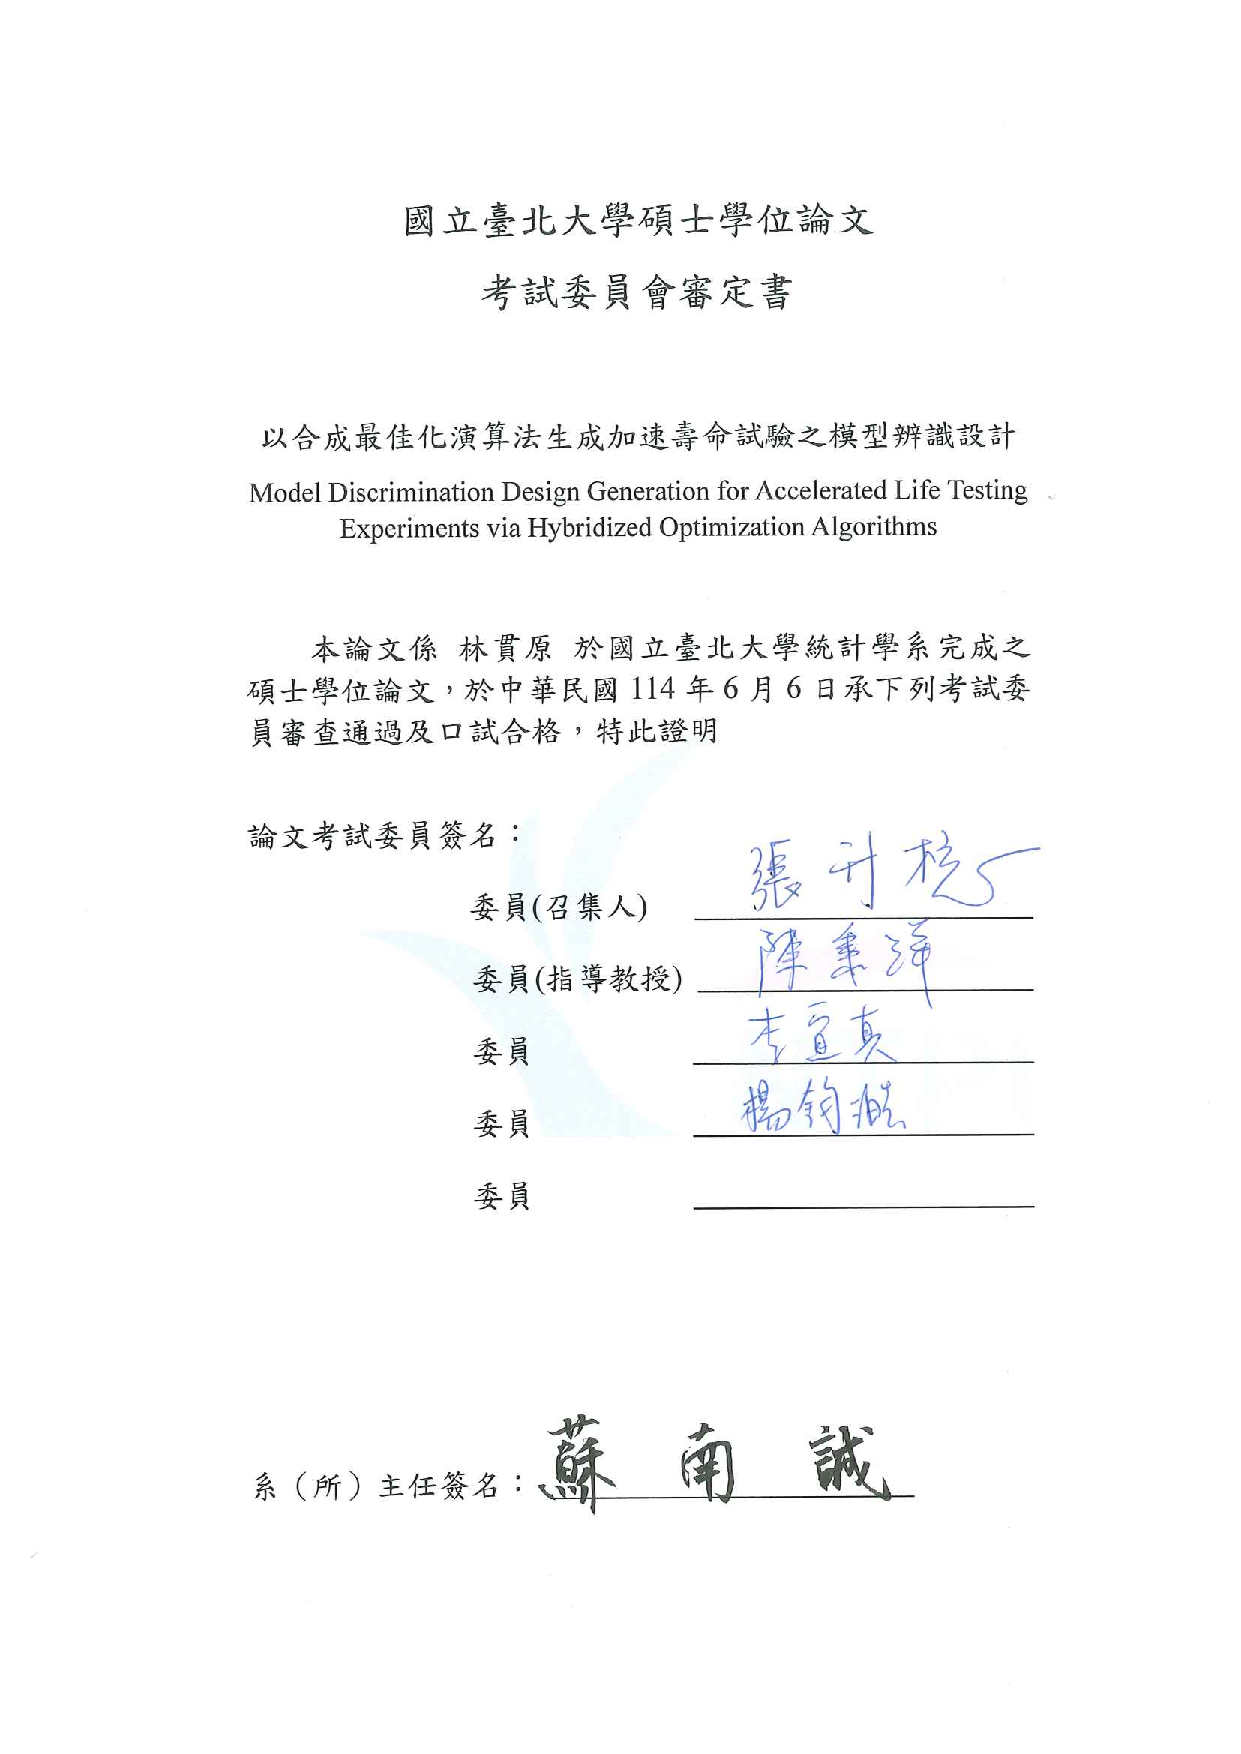
\includepdf[pages=1, pagecommand={}, fitpaper=true]{考試委員審定書.pdf}

\pagenumbering{roman}  
%\fancyhf{}
\fancyfoot[C]{\thepage}
\begin{center}
{\large 國立臺北大學一一三學年度第二學期碩士學位論文提要}
\fboxrule=1pt
\fboxsep=20pt
\fbox{\begin{minipage}{12cm}
\noindent 論文題目:~\underline{~~以合成最佳化演算法生成加速壽命試驗之模型辨識設計~~}

\noindent 論文頁數:~\underline{~~115~~}

\noindent 所~組~別:~\underline{~~統計學系碩士班~~}~~系(所)~~\underline{~~~~~~~~}~組~(學號:~\underline{~711233119~}~~)

\noindent 研~究~生:~\underline{~~~~林貫原~~~~}~~指導教授:~\underline{~~~~陳秉洋~~~~}

%\bigskip
\noindent 論文提要內容:
本研究旨在探討加速壽命試驗中,當存在多個候選模型可描述產品失效機制時,如何建構最適模型辨識設計。在此,於實驗設計的考量上,相較於對各候選模型參數的精準估計,如何能夠有效區分模型,確保所選模型貼近產品真實的失效機制,應為首要目標。加速壽命試驗透過施加高於正常使用條件的應力,以加速產品失效並在有限時間內取得壽命資料。然而,儘管進行加速,試驗結束時仍可能有樣本未發生失效,導致資料中出現設限現象。此類設限資料的特性,在既有模型辨識實驗設計的文獻中尚缺乏系統性的探討。
本研究首先探討在樣本可能為設限資料的情況下,如何建構最適模型辨識準則,基於改良後的 Kullback-Leibler 散度、Lin-Wong 散度、Chi-Square 距離與 Bhattacharyya 距離,提出 CKL-、CLW-、C$\chi^2$- 及 CB-最適模型辨識設計準則,以因應不同資料特性與應用需求。
另外,由於設計準則之數學結構複雜且為最大最小化的巢狀優化問題,不易推導最適設計之封閉解,本研究結合粒子群優化與梯度下降優化方法,構建一套高效的數值搜尋演算法,以尋找具最大模型辨識效力的實驗配置。為驗證方法之穩定性與有效性,本研究舉可靠度研究中常用的失效模型為案例進行數值實驗,考慮不同情境的失效機制與機率分布假設之候選模型,比較所提出之各種設計準則之模型辨識設計結果及效果,期望為後續可靠度試驗的實驗設計提供理論依據與實務參考。



%\vspace*{1.5cm}
\noindent 關鍵詞: 模型辨識設計、加速壽命試驗模型、粒子群優化演算法
\medskip
\end{minipage}}
\end{center}


\newpage
%\thispagestyle{empty}
\fontsize{12}{18pt}\selectfont
\begin{center}{\Large \bf ABSTRACT}\\[20pt]
    {\large MODEL DISCRIMINATION DESIGN GENERATION FOR ACCELERATED LIFE TESTING EXPERIMENTS VIA HYBRIDIZED OPTIMIZATION ALGORITHMS}\\[10pt]
    by\\[10pt] LIN,\,KUAN-YUAN\\[10pt] June 2025
\end{center}
{\small ADVISOR: Dr. CHEN, PING-YANG  \\[5pt]
        DEPARTMENT: DEPARTMENT OF STATISTICS\\[5pt]
        MAJOR: STATISTICS\\[5pt]
        DEGREE: MASTER OF SCIENCE}\\[10pt]
\noindent
This study aims to investigate the construction of optimal model discrimination designs in Accelerated Life Testing (ALT) when multiple candidate models are available to describe the product's failure mechanism. In this context, rather than focusing on the precise estimation of parameters within each candidate model, the primary objective of experimental design should be to effectively distinguish between competing models and ensure that the selected model closely reflects the true underlying failure behavior of the product. Accelerated Life Testing accelerates product failure by applying stress levels beyond normal use conditions, thereby enabling lifespan data to be collected within a limited timeframe. However, even under such accelerated conditions, some units may not fail by the end of the test, resulting in Type I censored data. The presence of censoring introduces unique data characteristics that have not been systematically addressed in the existing literature on model discrimination design. To address this gap, the present study first explores how to construct optimal model discrimination criteria under the possibility of Type I censored observations. Based on modified forms of Kullback–Leibler divergence, Lin–Wong divergence, Chi-square distance, and Bhattacharyya distance, we propose four new design criteria tailored for model discrimination under censoring: the CKL-, CLW-, C$\chi^2$-, and CB-optimal criteria. These criteria are designed to accommodate varying data characteristics and practical application needs. Due to the mathematical complexity of the proposed design criteria, each involving a nested max–min optimization problem, deriving closed-form solutions is generally intractable. To this end, we develop a computationally efficient numerical algorithm that combines Particle Swarm Optimization with gradient-based optimization methods to search for the optimal model discrimination designs. To validate the effectiveness of the proposed approach, we conduct numerical studies using commonly adopted failure models in reliability research. Through various scenarios of failure behavior and underlying probability distribution assumption of the candidate models, we show for each proposed criterion the resulting model discrimination designs and discuss their performances. The results are intended to provide both theoretical guidance and practical reference for experimental planning in future reliability studies.

\vspace*{2cm}
\noindent {\scshape KEY WORDS}: Model Discrimination Design, Accelerated Life Testing Model, Particle Swarm Optimization


   	

\newpage
\fontsize{12}{22pt}\selectfont 	
\fancyfoot[C]{\thepage}

\cleardoublepage
\setcounter{tocdepth}{2} 

\tableofcontents
\newpage
%\renewcommand{\numberline}[1]{\loflabel~#1\hspace*{1em}}
\listoffigures 
\newpage
%\renewcommand{\numberline}[1]{\lotlabel~#1\hspace*{1em}}
\listoftables 
\newpage

\ifodd\count0 \else \thispagestyle{empty}\mbox{}\clearpage\fi 
\pagenumbering{arabic} 		
\setcounter{page}{1} 
\chapter{緒論 \label{CH: intro}}

\hspace*{8mm} 在加速壽命試驗(Accelerated Life Testing, ALT)研究中,實驗設計的主要目標通常是提高參數估計的精度,例如透過 $c$-optimal 設計來最小化參數估計的變異。然而,當存在多個候選模型時,僅關注參數估計可能不足以確保模型的正確性。我們關注的核心問題是:如何設計實驗,使所收集的數據能有效區分不同的加速壽命模型,進而選擇最能反映產品實際失效行為的模型?這正是模型辨識設計(Model Discrimination Design)所要解決的關鍵挑戰。

\hspace*{8mm} 可靠度試驗是產品壽命分析中的重要環節,而 ALT 是透過施加高於正常使用條件的應力(如溫度、濕度、震動等)來加速產品老化,使研究人員能在有限時間內觀察失效現象。多數 ALT 模型以 Arrhenius 模型為基礎,假設壽命與溫度呈指數關係。然而,在實際應用中,可能存在多個結構不同但皆合理的模型,導致無法單靠既有經驗選定最佳模型。因此,如何透過設計適當的實驗條件,以產生能夠有效區分模型的資料,是 ALT 設計的重要議題。另一方面,即使在加速條件下進行試驗,產品仍可能未於測試期間發生失效,導致資料呈現 Type I 設限(Type I censored)現象。此時,研究者需設定合理的設限時間(censoring time),以控制試驗成本與時程,同時確保資料仍具備足夠資訊進行分析。因此,在考慮模型辨識設計時,設限資料的特性亦須一併納入評估。

\hspace*{8mm} 雖然模型辨識設計在其他領域已有所研究,但在 ALT 中仍相對較少受到關注。例如,\cite{nasir2015simulation} 提出的模型辨識方法主要基於貝葉斯最佳化策略,透過 Hellinger 距離來評估模型區分能力。然而,該方法在計算成本與結果穩定性方面仍存在挑戰,且主要聚焦於特定測試條件,未廣泛考慮不同類型的距離衡量準則。因此,本研究希望進一步探索加速試驗下的模型辨識問題,並考慮 Type I 設限數據(censored data)對實驗設計的影響。

\hspace*{8mm} 此研究第一個主要貢獻,在於提出四種基於不同散度的模型辨識設計方法,分別為 CKL-、CLW-、CB- 與 C$\chi^2$-optimal,這些準則皆針對設限情境下的實驗資料進行調整,期望提供更具彈性與準確性的模型選擇依據。

\hspace*{8mm} 如何生成模型辨識是這項研究的另一個關鍵。由於涉及的最佳化問題是嵌套的,並且通常缺乏目標函數的封閉解,我們進一步提出了一種高效的混合搜索演算法,結合粒子群優化(PSO)和基於牛頓法的方法,例如 L-BFGS 算法,以提高計算效率和收斂穩定性。我們展示了這種方法如何在合理的計算時間內識別出具有高模型區分能力的實驗設計,並通過數值模擬驗證其性能。

\hspace*{8mm} 本論文的架構如下:章節 \ref{CH: review} 回顧相關文獻,探討模型辨識設計的發展與現有最佳化標準。章節 \ref{CH: method} 提出我們的設計準則與最佳化演算法。章節 \ref{CH: simulation} 展示數值實驗結果,並比較不同設計標準在不同情境下的表現。章節 \ref{CH: conclusion} 則總結主要發現並提出了可能的未來研究方向。
\chapter{文獻回顧 \label{CH: review}}

\section{加速壽命試驗}

\hspace*{8mm} 生產高可靠性產品一直是製造業的重要目標之一。在產品研發的初期階段,確認產品壽命是否符合既定標準至關重要。然而,當預期壽命遠遠超過可測試的時間時,常用的方法是進行加速壽命試驗(Accelerated Life Testing, ALT)。該方法通過改變環境條件(例如提高溫度、增加振動頻率等)來加速產品的老化過程,並通過設定不同的應力條件來收集數據,結合數學模型外推產品在正常使用條件下的壽命分佈。例如,藥品穩定性試驗通常需在幾週內完成。根據 \cite{guideline2003stability} 指導文件,建議在高溫、高濕環境中進行加速測試,以 Pfizer 為例,在新藥研發中,該公司會通過加速穩定性試驗模擬 2 至 5 年的儲存條件。同樣地,電動車電池的目標壽命通常為 8 至 10 年或 100,000 公里以上,但由於實際測試無法覆蓋這麼長的時間,研究人員通常通過估計電池容量隨時間的衰減曲線,進一步外推電池在實際使用條件下的壽命。 \cite{uddin2017possibility} 在不同溫度與充放電速率下的加速試驗結果來模擬長期使用情境,用於預測鋰電池在實際駕駛條件下的性能衰退。

% 安定性試驗指引(Q1A) 是國際藥品法規協和會(International Conference on Harmonization, ICH)首批定稿的指引之一,早在1993 年進入第4階段1,接著在2000年代初期進行修訂2次為Q1A(R2)

\hspace*{8mm} \cite{arrhenius1889reaktionsgeschwindigkeit} 提出的 Arrhenius 模型為化學反應動力學奠定了理論基礎,並被廣泛應用於可靠度分析和 ALT 等領域。該模型描述了溫度對化學反應速率或產品壽命的影響,並假設產品的失效過程遵循 Arrhenius 方程。該方程表示為:
\begin{equation} \label{Arrhenius model}
t(T) = A \cdot \exp\left( \frac{E_a}{K \cdot Temp} \right),
\end{equation}

其中:
\begin{itemize}
\item $t(T)$:在溫度 $Temp$ 下產品的壽命;
\item $A$:頻率因子(Pre-exponential Factor),與產品的內在性質相關,是常數;
\item $E_a$:活化能(Activation Energy),表示驅動失效過程所需的能量,單位為電子伏特;
\item $K$:玻爾茲曼常數(Boltzmann Constant, $8.617 \times 10^{-5} \, eV/K$);
\item $Temp$:克爾文溫度(Kelvin, $^{\circ}\text{C}+273.15$)。
\end{itemize}

\hspace*{8mm} 該模型假設失效速率與溫度之間呈指數關係,表示在高溫條件下,失效速率顯著加快。這一特性使得 Arrhenius 模型成為 ALT 中的核心工具,透過高溫數據的收集,可以外推產品在正常使用條件下的壽命。然而,在實務應用中,模型的準確性受多種因素影響,特別是在實驗設計、參數估計與模型辨識方面存在挑戰。

\hspace*{8mm} 首先,溫度點的選擇是 ALT 中影響結果準確性的關鍵因素。如果所選的測試溫度過低,需要耗費大量時間和成本進行測試才能觀察到產品失效,無法有效縮短測試週期;反之,若溫度過高,雖可加速產品失效,但可能導致實驗條件與實際使用情境落差過大,降低結果的外推性與實用性。因此,如何在有限次數內選擇合適的溫度點成為一個重要課題。

\hspace*{8mm} 其次,在參數估計方面,活化能 $E_a$ 和頻率因子 $A$ 的準確性對於壽命預測至關重要。傳統上,透過最小平方估計(Least Squares Estimation, LSE)或最大概似估計(Maximum Likelihood Estimation, MLE)來推算參數。然而,在 ALT 中,設限數據(censored data)是無可避免的,因為測試時間有限,部分產品在測試結束時仍未失效。因此,標準估計方法可能不適用,必須考慮設限數據下的修正概似函數(Modified Likelihood Function),確保參數估計在 ALT 框架下的統計合理性。

\hspace*{8mm} 在 MLE 框架下,假設我們對 $j$ 個不同的溫度(應力)$T_j$ 下的樣本進行測試,並測量 $n$ 個個別樣本的壽命,所以我們記錄溫度 $T_j$ 下,第 $i$ 個樣本的壽命,記作 $t_{ij}$ 。我們認為壽命 $t_{ij}$ 服從 $Weibull(\lambda,\beta)$,其中 $\lambda_j$ 是對應溫度 $T_j$ 的尺度參數,因此需透過 Arrhenius 模型來決定,$\beta$ 是形狀參數(通常假設所有溫度條件下形狀參數相同):
% $t(T_j)$ 是在溫度 $T_j$ 下的平均壽命,$t_{ij}$則是個別產品在溫度 $T_j$ 下的實際測得壽命,這些數據服從 Weibull 分佈。
\begin{equation} \notag
f(t_{ij}; \lambda_j, \beta) = \beta \lambda_j t_{ij}^{\beta - 1} \exp(-\lambda_j t_{ij}^\beta)
\end{equation}

其中:
\begin{enumerate}
\item $\lambda_j$ 由 Arrhenius model 決定:
\begin{equation} \notag
\lambda_j = A^{-1} \exp\left(-\frac{E_a}{K T_j}\right)
\end{equation}
\item $\beta$ 是 Weibull 形狀參數(通常已知或額外估計)。
\end{enumerate}

若所有產品皆失效(無 Type I 設限數據),則概似函數(Likelihood Function)為:
\begin{equation} \notag
L(A, E_a, \beta) = \prod_{j} \prod_{i=1}^{n_j} f(t_{ij}; \lambda_j, \beta)
\end{equation}

對數概似函數(Log-Likelihood Function)為:
\begin{equation} \notag
\ell(A, E_a, \beta) = \sum_j \sum_{i=1}^{n_j} \left[ \ln \beta + (\beta - 1) \ln t_{ij} - \ln A - \frac{E_a}{K T_j} - A^{-1} e^{-\frac{E_a}{K T_j}} t_{ij}^\beta \right]
\end{equation}

\hspace*{8mm} 然而,在 ALT 中,部分樣本因時間限制而未失效,形成 Type I 設限數據,這時概似函數需考慮存活函數(Survival Function):
\begin{equation} \notag
S(t; \lambda_j, \beta) = \exp(-\lambda_j t^\beta)
\end{equation}

因此,修正後的概似函數為:
\begin{align}
L(A, E_a, \beta) &= \prod_{j} \prod_{i \in \text{失效}} f(t_{ij}; \lambda_j, \beta) \times \prod_{i \in \text{設限}} S(t_{ij}; \lambda_j, \beta) \notag \\
&= \prod_{j} \prod_{i \in \text{失效}} \beta \lambda_j t_{ij}^{\beta - 1} \exp(-\lambda_j t_{ij}^\beta) \times \prod_{i \in \text{設限}} \exp(-\lambda_j t_{ij}^\beta) \notag
\end{align}

取對數後,修正後的對數概似函數為:
\begin{align}
\ell(A, E_a, \beta) =& \sum_j \sum_{i \in \text{失效}} \left[ \ln \beta + (\beta - 1) \ln t_{ij} - \ln A - \frac{E_a}{K T_j} - A^{-1} e^{-\frac{E_a}{K T_j}} t_{ij}^\beta \right] \notag \\
&- \sum_j \sum_{i \in \text{設限}} A^{-1} e^{-\frac{E_a}{K T_j}} t_{ij}^\beta \notag
\end{align}

\hspace*{8mm} 換句話說,ALT 中的參數估計必須與 Type I 設限數據對應的概似函數共同調整,才能獲得穩健的結果。目標是估計影響產品壽命的關鍵參數 $A$、$E_a$ 和 $\beta$,我們需要尋找修正後對數概似函數達到最大值的參數估計值 $\hat{A}, \hat{E}_a, \hat{\beta}$:

為了得到最適合 ALT 數據的參數估計值,我們透過解以下方程組來估計:

$$\frac{\partial \ell}{\partial A} = 0, \quad \frac{\partial \ell}{\partial E_a} = 0, \quad \frac{\partial \ell}{\partial \beta} = 0$$

透過 MLE 獲得的參數 $\hat{A}, \hat{E}_a, \hat{\beta}$ 能夠確保 ALT 模型的準確性,進而有效推估產品在正常操作條件下的壽命。

在過去的研究中,$c$-optimal設計被廣泛應用,其主要目標是透過選擇最佳的實驗條件(如溫度點),最小化關鍵參數的估計變異。特別是在 ALT 研究中,$c$-optimal 設計被廣泛用於提高活化能 $E_a$ 的估計精度,以確保壽命模型的可靠性。

例如:
\begin{enumerate}

\item \cite{lu2019bayesian} 提出了一種基於雙重目標的貝葉斯序貫設計方法,結合 D-optimal 和 $c$-optimal 準則,前者應用於實驗的早期階段,以快速提高模型參數估計的精度,後者則在後期階段專注於最小化特定壽命分位數(如第 $p$ 百分位壽命)的估計變異,確保壽命預測的穩定性與準確性。

\item \cite{abd2020optimal} 探討了$c$-optimal 設計在多重加速壽命試驗(Multiple ALT)中的應用,並比較了不同最佳化準則(D-, $c$-, A-optimal)在實驗設計效能上的表現,同時進行了敏感性分析(sensitivity analysis)來評估錯誤參數設定對設計結果的影響。

\item \cite{newer2024optimal} 研究了$c$-optimal 設計在 ALT 中的應用,特別是在漸進 Type-I 設限(Progressive Type-I Censoring, PTIC)條件下。他們比較了多種最佳化準則(D-, E-, T-, $c$-, R-, P-optimal),並發現$c$-optimal 方法能夠有效最小化壽命分佈的特定參數(如 Weibull 分佈中的尺度參數 $\lambda_0$)的估計變異。研究結果顯示,$c$-optimal 設計在步進應力加速壽命試驗(SALT)中,能夠在測試資源有限的條件下,提高壽命分佈關鍵參數的估計精度。

\end{enumerate}

\hspace*{8mm} 最後,在 ALT 研究中,模型辨識問題往往被忽視。雖然 Arrhenius 模型在許多溫度加速試驗中廣泛應用,但在某些產品或材料中,高溫可能會觸發額外的物理或化學機制,導致失效模式發生變化。例如,在某些電子元件中,高溫可能不僅加速老化,還可能引發電遷移(Electromigration)或介電層破壞(Dielectric Breakdown),這些失效機制未必能完全由 Arrhenius 模型準確描述。因此,如何透過實驗數據檢驗 Arrhenius 模型的適用性,並考慮可能的替代模型,是 ALT 設計中不可忽視的課題。

\hspace*{8mm} 然而,我們發現現有研究多關注於提升參數估計的精度,例如透過$c$-optimal 設計來提高模型參數的估計效率,但較少考慮當兩個模型同樣基於 Arrhenius 框架,但其數學結構存在差異時,如何設計實驗來有效區分這些模型。這引出了另一個重要問題:是否能夠透過實驗設計,使未來的數據能夠有效區分這類競爭模型?這類方法被稱為模型辨識設計(Model Discrimination Design),其核心目標是選擇合適的實驗條件,使不同模型在觀測數據上的行為產生顯著差異,從而提升模型選擇的準確性。

\section{模型辨識設計}

\hspace*{8mm} 在實務應用上,無論是科技業、製造業,或其他快速發展的領域,其發展變化的速度往往呈現指數級增長。在此背景下,原本所採用的模型可能因環境變化而逐漸失去適用性,導致模型的預測準確度下降,甚至影響決策的有效性。因此,如何判斷應該繼續沿用現有模型,還是更新為更能反映當前環境的新模型,成為一項重要課題。為了做出最佳決策,模型辨識設計可用來比較不同模型的適用性。在面對新的環境變數時,決策者不應單純地捨棄舊模型或全面採用新模型,而應透過嚴謹的統計方法,客觀評估各種模型的適用性,確保選擇的模型能夠有效反映當前情境,進而提升決策的準確性與可靠性。

\hspace*{8mm} \cite{atkinson1975design,atkinson1975optimal} 提出了用於區分兩個對立模型的實驗設計方法,假設模型服從常態分佈,並提出了T-optimal 設計。假設現在有兩個高斯模型,它們具有相同的變異數 $\sigma^2$ 但不同的平均反應函數,分別為 $\eta_1(x, \theta_{1})$ 和 $\eta_2(x, \theta_{2})$ 。希望比較這兩個模型。在實務中,第一個模型通常被認為是已知的,可能來自於專家的意見或基於過往經驗的現有現狀。因此,我們假設第一個模型是真實模型,並記其參數為已知的 $\theta_1=\theta_{tr}$ ,即 $\eta_{tr}(x)=\eta_1(x, \theta_{tr})$ 。第二個模型則是對立模型,記為 $\eta_r(x, \theta_{2})=\eta_2(x, \theta_{2})$,其中 $\theta_2\in \Theta_2$是未知的。

\hspace*{8mm} 為了在沒有資料的情況下進行模型辨識,採用了 T-optimal 設計標準,其目標函數如公式 \eqref{eq:T-optimal-1} 所示:
\begin{equation}\label{eq:T-optimal-1}
T_{2,tr}(\xi)=\min_{\substack{\theta_2\in \Theta_2}}\int_{X}\Delta_{2,tr}(x,\theta_2) \xi(dx)
\end{equation}

其中,$\Delta_{2,tr}(x,\theta_2)=\left[\eta_{tr}(x)-\eta_2(x,\theta_2)\right]^2$,$\xi$ 是實驗設計的分佈。我們的目標是選擇一個設計分佈 $\xi$,使得當我們最小化 $\theta_2$ 引起的模型差異後,兩個模型的差異仍然足夠大,以便後續的數據分析能清楚地區分這兩個模型。

\hspace*{8mm} 然而,T-optimal 設計的目標僅僅是在最小化兩個模型對應於 $\theta_2$ 的差異情況下進行設計,但我們希望進一步確保所選設計在未來收集到數據後,兩個模型的差異只會更加顯著。因此,我們提出一個基於最大化策略的設計方法,這導致了目標函數的調整,如公式 \eqref{eq:T-optimal-2} 所述:
\begin{equation}\label{eq:T-optimal-2}
\max_{\xi\in \Xi} T_{2,tr}(\xi)=\max_{\xi\in \Xi} \min_{\substack{\theta_2\in \Theta_2}}\int_{X}\Delta_{2,tr}(x,\theta_2) \xi(dx)
\end{equation}

\hspace*{8mm} 這一方法的核心思想是在選擇設計分佈 $\xi$ 時,先針對每個可能的 $\theta_2$ 找到模型間差異的最小值,然後在所有可能的設計中選擇能最大化該最小差異的 $\xi$ 。此設計目標的意圖在於,無論未來收集到的數據如何影響 $\theta_2$ 的估計,兩個模型之間的實際差異只會比設計階段考慮的最小差異更大。因此,這樣的設計不僅有助於解決當前的模型辨識問題,還能提高未來實驗數據的利用效率,為模型選擇提供更強的支持。

\begin{theorem}
為了驗證找到的設計 $\xi_T^\ast$ 是否為最佳設計,我們使用等價定理(Equivalence Theorem, \citep{atkinson1975design,atkinson1975optimal}),如公式 \eqref{eq:T-optimal-3} 所示:
\begin{equation}\label{eq:T-optimal-3}
\psi_T(x, \xi_T^\ast) = \Delta_{2,tr}(x, \hat{\theta}_2(\xi_T^\ast)) - T_{2,tr}(\xi_T^\ast) \leq 0,
\end{equation}

其中:
\begin{itemize}
\item 第一項 $\Delta_{2,tr}(x, \hat{\theta}_2(\xi_T^\ast))$ 表示在設計空間 $\mathcal{X}$ 的每一點 $x$ 上,針對所有可能的 $\theta_2 \in \Theta_2$ 計算模型差異的最小值。

\item 第二項 $T_{2,tr}(\xi_T^\ast)$ 是基於所選設計 $\xi_T^\ast$ 計算出的模型差異的最小值,這是經由「max-min」最佳化過程確定的全域最佳標準。
\end{itemize}
\end{theorem}

\hspace*{8mm} 如果對於所有 $x \in \mathcal{X}$,不等式 $\psi_T(x, \xi_T^\ast) \leq 0$ 成立,則可以確認 $\xi_T^\ast$ 是 T-optimal 設計。這表明,在任何設計點上,局部模型差異的最大值都不會超過全局模型差異,從而確保設計的最佳性。

\hspace*{8mm} 然而, \cite{atkinson1975design,atkinson1975optimal} 提出的 T-optimal 設計旨在通過最大化模型之間差異平方和,實現對模型的有效辨識。然而,該方法在某些應用情境下存在限制。例如,當兩個模型的變異不同或誤差項不符從常態分佈時,僅考慮差異平方和可能不足以充分反映模型之間的差異。此時應考慮分佈整體形狀的差異,這可以通過 Kullback-Leibler 散度(KL Divergence)來衡量模型之間的資訊損失。 \cite{lopez2007optimal} 針對此類情況提出了 KL-optimal 設計,並通過模擬不同條件下的情境,尋找適用於模型辨識的有效設計。

\section{尋找模型辨識設計的數值方法}

\hspace*{8mm} 在尋找最佳化的過程中,\cite{atkinson1975design,atkinson1975optimal} 採用了類似交換演算法的增量式設計。然而,在處理連續型設計空間時,該方法通常需先設定一組基準設計(例如隨機選取三個設計點)作為起始點。接著,演算法會從預先離散化的設計空間中(例如每隔 50 或 100 單位切分)選出候選點,逐一嘗試加入目前設計中,觀察是否能提升準則值,若有提升則保留該點。經過反覆遞迴後,最終設計可能出現多個非零權重的支撐點,甚至集中於部分區段,導致支撐點總數超出原本預期(例如原本為三點設計)。此外,若鄰近點如 99、100、101 皆帶有小權重,可能在圖形上呈現「多點集中於一區」的特性。這些現象使得交換演算法在支撐點數量與設計可解釋性上較難控制。

\hspace*{8mm} 此外,綜合上述前人研究的成果與分析,以及不論是 T-optimal 設計還是 KL-optimal 設計,其極值求解過程可能耗費大量時間,對計算效率提出了挑戰。因此,採用更加高效的連續型優化演算法是一個值得探索的方向。近十年來的研究顯示,粒子群優化(Particle Swarm Optimization, PSO)在處理實驗設計問題上具有顯著優勢,能夠解決許多過去理論或傳統演算法無法有效解決的問題。因此,本研究將採用 PSO 演算法作為求解工具,以提升計算效率與結果的準確性。值得一提的是,\cite{chen2020hybrid} 已成功應用 PSO 演算法於模型辨識問題,啟發了本研究嘗試將此方法套用於可靠度領域中最常見的 Arrhenius 模型,以探索其在該領域的應用潛力。

\hspace*{8mm} \cite{eberhart1995new} 首次提出粒子群優化方法,這是一種啟發式優化演算法,靈感來自於自然界中魚群與鳥群的集體行為。PSO 將每隻鳥或每條魚視為一個粒子,每個粒子代表一個候選解。通過結合自身歷史最佳解(Local Best, LBest)和群體全局最佳解(Global Best, GBest)的資訊,接著持續調整速度與位置,最終逐漸收斂至全局最佳解。針對不同類型的最佳化設計,已有眾多文獻應用 PSO 方法進行研究。例如,\cite{chen2011optimal} 探討了 A-optimal、D-optimal 和 Minimax 設計;\cite{lukemire2016using} 將 PSO 用於尋找 D-optimal 設計;\cite{walsh2022fast} 則研究了 G-optimal 設計等。

\hspace*{8mm} PSO 的迭代過程包含兩個主要步驟,首先初始化粒子的速度與位置,然後根據公式 \eqref{eq:PSO_1} 計算粒子的速度,接著利用公式 \eqref{eq:PSO_2} 更新粒子的位置。在這一過程中,粒子的運動由三個關鍵組成部分構成,概念如圖 \ref{fig:PSO velocity} 所示:

\begin{itemize}
\item $\textcolor{PowerPointGreen}{(A)}$:慣性項,表示粒子的運動趨勢,通過延續前一次的速度影響當前速度。
\item $\textcolor{blue}{(B)}$:個體學習項,通過粒子自身的歷史最佳位置 ($\xi_L^{t}$, LBest) 引導粒子向更好的解移動。
\item $\textcolor{red}{(C)}$:群體學習項,通過群體的全局最佳位置 ($\xi_G^{t}$, GBest) 協助粒子向全局最佳解靠近。
\end{itemize}

粒子 $i$ 在時間 $t$ 和 $t+1$ 的運動由以下公式控制:
\begin{equation}\label{eq:PSO_1}
v_i^{t+1} = \underbrace{\varphi_{t} v_i^{t}}_{\textcolor{PowerPointGreen}{\text{(A)}}} + \underbrace{\gamma_1 \beta_1 \otimes \left[ \xi_{L}^{t} - \xi_i^{t} \right]}_{\textcolor{blue}{\text{(B)}}} + \underbrace{\gamma_2 \beta_2 \otimes \left[ \xi_G^{t} - \xi_i^{t} \right]}_{\textcolor{red}{\text{(C)}}}
\end{equation}
和
\begin{equation}\label{eq:PSO_2}
\xi_i^{t+1} = \xi_i^{t} + v_i^{t+1}, \quad \text{for } i = 1, \dots, N.
\end{equation}

\hspace*{8mm} 在公式 \eqref{eq:PSO_1} 中,$v_i^{t}$ 和 $v_i^{t+1}$ 分別代表粒子 $i$ 在時間 $t$ 和 $t+1$ 的速度;$\varphi_{t}$ 是慣性權重,其值介於 0 和 1 之間,可以是常數,也可以是隨時間遞減的函數。通常,在算法初期,較大的慣性權重有助於提升全局搜索能力,防止粒子過早陷入局部最佳解;而在算法後期,使用較小的慣性權重則有助於粒子進行精細搜索,提高解的精度並加速收斂。學習因子 $\gamma_1$ 和 $\gamma_2$ 分別對應個體學習和群體學習,控制粒子向 LBest 和 GBest 的移動權重,兩者通常設定為常數。而隨機數 $\beta_1$ 和 $\beta_2$ 是從均勻分佈 $U(0,1)$ 中隨機生成的,用於引入隨機性,增加粒子搜索的多樣性。

\begin{figure}[H]
    \centering{
        \includegraphics[scale=0.3]{\imgdir PSO detail.png}}
    \caption{PSO 速度運動示意圖}
\label{fig:PSO velocity}
\end{figure}

PSO 演算法流程:(可參考圖 \ref{fig:PSO concept} )

\begin{enumerate}
\item 初始化粒子:
\begin{enumerate}[→]
    \item 生成粒子群,包含 $n$ 個粒子。
    \item 初始化粒子的位置 $\xi_i$ 和速度 $v_i$,其中 $i = 1, \dots, n$。
    \item 確認每個粒子的自身歷史最佳解($\xi_L^{t}$, LBest)以及群體全局最佳解($\xi_G^{t}$, GBest)。
\end{enumerate}

\item 迭代過程:
\begin{enumerate}[→]
\item 運用公式 \eqref{eq:PSO_1} 計算每個粒子的速度。
\item 運用公式 \eqref{eq:PSO_2} 更新粒子的位置。
\item 每個粒子基於優化目標函數計算適應度值,並更新其 LBest 和 GBest。
\item 判斷是否滿足停止條件(如達到迭代次數或適應度收斂),否則重複上述步驟。
\end{enumerate}

\item 輸出結果:
\begin{enumerate}[→]
    \item 以群體全局最佳解(GBest) 作為最終結果。
\end{enumerate}
\end{enumerate}

\begin{figure}[H]
    \centering{
        \includegraphics[scale=0.4]{\imgdir PSO concept.png}}
    \caption{PSO 流程圖}
\label{fig:PSO concept}
\end{figure}

\section{現有應用於 ALT 的模型辨識設計方法}

\hspace*{8mm} 在 ALT 研究中,模型辨識問題相對較少被探討,而 \cite{nasir2015simulation} 是其中較具代表性的研究之一。該研究針對 ALT 中的模型辨識問題,提出了一種基於貝葉斯方法(Bayesian Approach)的最佳化實驗設計策略,重點在於如何透過實驗設計來區分競爭模型,特別是在壽命與應力變數之間的關係可能為線性或非線性,且結構不確定的情境。他們採用 Hellinger 距離(Hellinger distance)衡量不同模型預測分佈之間的差異,並透過數值模擬來驗證該設計的有效性。

\hspace*{8mm} 首先,透過圖 \ref{fig:ALT concept} 簡要說明 ALT 的概念。假設目前有兩個模型 $M_1$ 和 $M_2$,目標是預測產品的壽命第 $p$ 百分位數($\tau_p$)。然而,當產品在正常使用條件下的壽命過長,難以在短時間內獲得失效數據時,通常會透過提高應力(stress)來加速產品故障,以縮短測試時間。  

\hspace*{8mm} 在實驗設計中,設定兩個應力水準,分別為低應力($S_{Low}$)和高應力($S_{High}$),並在這些條件下測試產品的失效數據分佈。接著,利用外推方法預測在實際使用應力 $S_{UC}$ 下的失效分佈,進而推估產品的壽命。

\hspace*{8mm} 圖中橫軸代表應力,縱軸代表產品壽命,兩者皆取對數,主要是因為許多壽命模型(如 Arrhenius 模型)呈現非線性關係,透過對數轉換可將其轉換為線性關係,便於進行統計推論。此外,在高應力條件下,產品壽命的變異性較大,數據分佈可能呈現高度偏態(Skewed),而對數變換後,壽命數據通常更接近常態分佈,有助於提高模型的適用性與參數估計的穩定性。因此,對 $M_1$ 和 $M_2$ 進行相同的實驗測試,觀察它們在不同應力條件下的壽命第 $p$ 百分位數($\tau_p$),並分析兩者的對數變換後的壽命分佈變化 $\Delta\hat{\tau_p}$,使不同模型在不同應力條件下的行為變化更直觀,進而幫助進行模型辨識。 以下將依序描述該研究中模擬步驟的詳細資訊。
 
\begin{figure}[H]
    \centering{
        \includegraphics[scale=0.6]{\imgdir ALT concept.png}}
    \caption{ALT 概念圖 \citep{nasir2015simulation}}
\label{fig:ALT concept}
\end{figure}

\hspace*{8mm} 目前的情境是,可靠度工程師對研究半導體組裝中 Au-Al 介面的金屬間化合物(IMC)生長感興趣。已知該故障機制會受到溫度應力的影響,因此需要進行加速壽命測試來估計設備的使用壽命,計劃能夠在溫度應力下區分線性模型 $M_1$ 和二次加速模型 $M_2$ ,其參數分別為 $\theta_1$ 和 $\theta_2$ 。實驗的設備與測試條件如下:

\begin{itemize}
\item 烘烤室有效期: 總測試時間為 42 天,即最長可達 1008 小時。

\item 可使用的兩種烤箱類型:

\begin{itemize}
\item 低應力烤箱:溫度範圍為 $60^{\circ}\text{C}$ 至 $115^{\circ}\text{C}$。
\item 高應力烤箱:溫度範圍為 $100^{\circ}\text{C}$ 至 $250^{\circ}\text{C}$。
\end{itemize}

\item 實驗成本限制: 最多可進行 20 次實驗。

\end{itemize}

本研究基於其論文中的真實工業案例,並提供詳細的模擬設置,包括以下所有要點。

\begin{enumerate}
\renewcommand{\labelenumi}{\Roman{enumi}.}

\item 調整模型形式並設定欲比較的模型:

首先,我們將 Arrhenius 模型(式 \eqref{Arrhenius model})線性化,以建立模型。
\begin{align}
&t(T)=Aexp\left( \frac{E_a}{K \times Temp} \right)\notag \\ 
\Rightarrow&\log(t(T))=\log(A)+\frac{E_a}{K \times Temp}\notag \\ 
\Rightarrow&\underbrace{\log(t(T))}_{\mu}=\underbrace{\log(A)}_{\beta_0}+\underbrace{\frac{E_a}{K}}_{\beta_1} \times \underbrace{\frac{1}{Temp}}_x \label{M2 linearized}
\end{align}

接著,對加速變數進行標準化,式 \eqref{M2 linearized} 可以擴展為:
\begin{align}
\overbrace{\log(t(T))}^{\mu}&=\overbrace{(\beta_0+\beta_1 x_{low})}^{\gamma_0}+\overbrace{\left[\beta_1(x_{high}-x_{low})\right]}^{\gamma_1}\overbrace{\left( \frac{x-x_{low}}{x_{high}-x_{low}}\right)}^{\xi} \label{M2 normalized}
\end{align}

加入二次項,以捕捉可能的非線性加速效應,可表示為:
\begin{equation} \label{M1 linearized}
\mu =\beta_0+\beta_1x+\beta_2x^2
\end{equation}

將式 \eqref{M1 linearized} 的加速變數進行標準化後,擴展為:
\begin{align}
\overbrace{\log(t(T))}^{\mu}=&\overbrace{(\beta_0+\beta_1 x_{low})}^{\gamma_0}+\overbrace{\left[\beta_1(x_{high}-x_{low})\right]}^{\gamma_1}\overbrace{\left( \frac{x-x_{low}}{x_{high}-x_{low}}\right)}^{\xi} \notag \\
&+\underbrace{\left[\beta_2 (x_{high}^2-x_{low}^2) \right]}_{\gamma_2}\underbrace{\left( \frac{x-x_{low}}{x_{high}-x_{low}}\right)^2}_{\xi^2} \label{M1 normalized}
\end{align}

綜合上述推導,方程式 \eqref{M2 normalized} 嵌入於 \eqref{M1 normalized} 之中,表示 $M_2$ 是$M_1$ 的一個特例。因此,我們定義 $M_1$ 和 $M_2$ 如下:
\begin{align}
M_1:\mu_1&=\gamma_0+\gamma_1 \xi +\gamma_2 \xi^2   \label{Final M1 normalized} \\
M_2:\mu_2&=\gamma_0+\gamma_1 \xi   \label{Final M2 normalized}
\end{align}

另外,可靠度工程師認為 Weibull 分佈能充分描述半導體封裝中 Au-Al 金屬間化合物的生長壽命及其失效機制。因此,他們假設壽命 $T$ 服從 Weibull 分佈, $T\sim Weibull(\alpha,\beta)$,其中 $\alpha$ 為尺度參數,$\beta$ 為形狀參數。進一步透過對數轉換,將壽命轉換為最小極值分佈(SEV),$\log(t)\sim SEV(\mu,\sigma)$,其中 $\sigma=\frac{1}{\beta}$ 且 $\mu=\log(\alpha)$。

對於兩個模型,對於 Type I 設限資料的情況下,超過時間 $t_c$ 的生存機率可表示為:
\begin{equation} \label{censored}
Pr(t>t_c)=exp\left[-\left(\frac{t_c}{\alpha}\right)^\beta\right],t_c>0
\end{equation}

\item 機率分佈的距離測度:

該研究採用 Hellinger 距離測量圖 \ref{fig:ALT concept} 中的 $\Delta\hat{\tau_p}(S_{Low})$ 和 $\Delta\hat{\tau_p}(S_{High})$ 的距離,假設目前兩個模型的壽命數據分別為 $Y_1=(y_{11},y_{21}, \dots, y_{N1})$ 和 $Y_1=(y_{12},y_{22}, \dots, y_{N2})$,且兩者皆有 $N$ 筆資料。Hellinger 距離的定義如下:
\begin{equation}
D_H(Y_1,Y_2)=\frac{1}{\sqrt{2}}\sqrt{\sum_{i=1}^N(\sqrt{y_{i1}}-\sqrt{y_{i2}})^2}
\end{equation}

\item 效用函數定義:研究進一步定義需最大化的效用函數,該函數考慮了在低應力和高應力下的實驗情境,並利用兩個模型的數據 $Y_1$ 和 $Y_2$ 進行綜合評估。
\begin{equation}
u_{2|1}=D_{S_{Low}}(\hat{\tau}_{p,(M_2|Y_1)},\hat{\tau}_{p,(M_1|Y_1)}) +D_{S_{High}}(\hat{\tau}_{p,(M_2|Y_1)},\hat{\tau}_{p,(M_1|Y_1)})
\end{equation}
\begin{equation}
u_{1|2}=D_{S_{Low}}(\hat{\tau}_{p,(M_1|Y_2)},\hat{\tau}_{p,(M_2|Y_2)}) +D_{S_{High}}(\hat{\tau}_{p,(M_1|Y_2)},\hat{\tau}_{p,(M_2|Y_2)})
\end{equation}

\item 效用函數的期望調整:由於在設計實驗時尚未觀察到真實數據,因此透過數據的抽樣分佈 $p(y_1|\theta_1)$ 和 $p(y_2|\theta_2)$,搭配參數的先驗分佈 $\pi(\theta_1)$ 和 $\pi(\theta_2)$,計算效用函數的期望值:
\begin{equation}
E(u_{2|1})=\int\int u_{2|1}p(y_1|\theta_1)\pi(\theta_1)d_{y_1}d_{\theta_1}
\end{equation}
\begin{equation}
E(u_{2|1})=\int\int u_{2|1}p(y_1|\theta_1)\pi(\theta_1)d_{y_1}d_{\theta_1}
\end{equation}

\item 模型權重與最終效用函數:由於尚不清楚哪個模型是真實的,因此引入模型權重的先驗分佈 $\tau(M_1)$ 和 $\tau(M_2)$,最終效用函數 $U(\xi)$ 可表示為:
\begin{equation}
U(\xi)=\tau(M_1)E(u_{2|1})+\tau(M_2)E(u_{1|2})
\end{equation}

透過最大化 $U(\xi)$,可以確保設計能夠最大化兩個模型之間的差異性。

\item 給定先驗分佈:

\begin{itemize}

\item 假設兩個模型的初始可信度相等,設定 $\tau(M_1) = \tau(M_2) = 0.5$。
\item 假設活化能遵循均勻分佈,$E_a \sim U(1.0, 1.05)$,表示其可能值範圍在 1.0 到 1.05 eV 之間,並且各值的機率相同。
\item 假設 $\beta_0$ 服從平均數為 0、變異數為 $1000^2$ 的常態分佈,$\beta_0 \sim N(0, 1000^2)$,反映對該參數高度不確定的假設。
\item 同樣假設二次項 $\beta_2$ 服從 $\beta_2 \sim N(0, 1000^2)$,允許其具有廣泛的可能值。
\item 假設壽命數據遵循 Weibull 分佈,其形狀參數 $\beta$ 服從伽瑪分佈,$\beta \sim Gamma(1,2)$。

\end{itemize}

\end{enumerate}

\hspace*{8mm} 他們採用了基於貝葉斯方法的模擬技術,通過不斷抽取資料來估計經驗分佈的形狀,進而計算不同分佈之間的差異。在此過程中,他們使用了馬可夫鏈蒙地卡羅(Markov Chain Monte Carlo, MCMC)方法中的 Gibbs 抽樣,並利用 WinBUGS 軟體來計算 $\hat{\tau}_p$ ,同時模擬最大化效用函數以找到最佳設計 $\xi^*$ 。

\hspace*{8mm} 然而,該方法存在兩個主要缺點。首先,計算過程極為耗時,特別是在高維數據或大規模樣本情況下會顯著增加計算成本。其次,由於方法本身的隨機性,每次模擬的結果可能有所差異,導致難以復現先前的結果,這進一步限制了該方法的應用範圍。

\hspace*{8mm} \cite{nasir2015simulation} 在其研究中探討了模型辨識設計在可靠度測試中的應用。然而,綜上所述,其方法仍有許多待改進之處。因此,本研究將以該文獻的改進方向為出發點,進行深入探討。
%\chapter{Optimal Design Criteria \label{CH: method}}
\chapter{Methodology \label{CH: method}}

\hspace*{8mm} This study focuses on approximation designs, which are widely recognized for their practicality in experimental design. Approximation designs are probability measures defined over the design space $\mathcal{X}$, used to allocate limited observations across specific design points. Let the response variable $y$ follow a conditional probability distribution $f(y \mid x, \theta, \sigma^2)$, where $x$ represents a design point (support point) from the design space, such that $x \in \mathcal{X}$, $\theta$ denotes all unknown parameters, and $\sigma^2$ is the variance of the errors, treated as a nuisance parameter.

\hspace*{8mm} When the design points are $x_1, x_2, \dots, x_n \in \mathcal{X}$, an approximation design $\xi$ can be expressed as:
$$
\xi = \left\{\begin{array}{cccc}
x_1 & x_2 & \dots & x_n \\
w_1 & w_2 & \dots & w_n
\end{array}\right\}.
$$
\hspace*{8mm} Here, $w_i$ represents the weight assigned to the design point $x_i$, satisfying $0 < w_i < 1$ and $\sum_{i=1}^n w_i = 1$, where $i = 1, 2, \dots, n$. If the total sample size is $N$, the number of observations allocated to the design point $x_i$ is approximately $N \cdot w_i$, typically rounded to the nearest integer in practice. The objective of approximation designs is often based on convex or concave functions, allowing optimization algorithms to efficiently identify the best designs, which is denoted as $\xi^*$. Additionally, to confirm whether the obtained design is optimal, this study will employ the Equivalence Theorem as a verification tool.

\section{KL-optimal Criterion}

\hspace*{8mm} When the two models have different variances or the error terms do not follow a Normal distribution, \cite{lopez2007optimal} proposed the KL-optimal design to address such cases. This design measures the information loss between models using Kullback-Leibler divergence (KL divergence), which is also referred to as relative entropy, information divergence, or information gain. As the name suggests, it is closely related to entropy. The following sections will introduce different related metrics in sequence.

\hspace*{8mm} \cite{shannon1948mathematical} proposed information entropy as a measure of the uncertainty or information content in a probability distribution. Information content, $I(x)$, can be viewed as a surprise index: when the probability $P(x)$ of an event occurring is low, the occurrence of the event surprises us (high information content); conversely, when $P(x)$ is high, the occurrence of the event is expected, resulting in lower information content.

For example:

\begin{itemize}
\item A sunny day in the desert tomorrow → This is expected, as the probability is high (close to 1), so the information content is low.
\item Rain in the desert tomorrow → This is a rare event, with a low probability (close to 0), so the information content is high.
\end{itemize}

\hspace*{8mm} Therefore, when $P(x)$ approaches 0, indicating the event is highly unlikely to occur and the surprise level is high, the information content value must be large; when $P(x)$ approaches 1, the information content value must be small.

The definition of information content is:
\begin{equation}\label{eq:information content}
I(x)=-\log P(x).
\end{equation}

\hspace*{8mm} Entropy represents the average information content, as events usually do not occur in isolation and require comprehensive consideration. Assuming we consider the first model (true model) $f_{tr}(y \mid x, \sigma^2_1)$, its information entropy is defined as:
\begin{equation}\label{eq:information entropy}
H(f_{tr}) = -\int f_{tr}(y \mid x, \sigma^2_1) \log \left\{f_{tr}(y \mid x, \sigma^2_1)\right\} dy.
\end{equation}

\hspace*{8mm} A higher value of $H(f_{tr})$ indicates greater variability in the distribution, meaning that more information is obtained when an event occurs. Intuitively, information entropy can be interpreted as the amount of information gained after an event takes place. Since probability values range between $0$ and $1$, taking the logarithm results in negative values. Therefore, a negative sign is introduced in the formula to ensure that $H(f_{tr})$ remains non-negative. A larger entropy value suggests greater variability in the probability distribution and a higher amount of information provided by the occurrence of an event, whereas a smaller entropy value indicates less information.

\hspace*{8mm} Cross entropy measures the difference between the observed predicted probability distribution and the true probability distribution. Intuitively, it quantifies the additional information loss incurred when using one model to describe the true distribution. Consider the first model (true model) $f_{tr}(y \mid x, \sigma^2_1)$ and the second model (rival model) $f_r(y \mid x, \theta_2,\sigma^2_2)$. The cross entropy is defined as:
\begin{equation}\label{eq:cross entropy}
H(f_{tr},f_r) = -\int f_{tr}(y \mid x, \sigma^2_1) \log \left\{f_r(y \mid x, \theta_2,\sigma^2_2)\right\} dx.
\end{equation}

\hspace*{8mm} Cross entropy measures the average information loss when we approximate the true distribution $f_{tr}(y \mid x, \sigma^2_1)$ with a rival model $f_r(y \mid x, \theta_2,\sigma^2_2)$. A larger cross entropy value indicates a greater discrepancy between the two distributions, implying higher uncertainty and requiring more information to describe $f_{tr}(y \mid x, \sigma^2_1)$. Conversely, if the two distributions are similar, the cross entropy value will be lower, indicating that the rival model describes the true distribution more accurately. It is important to note that the minimum value of cross entropy is usually not zero; when the two models are identical, the cross entropy $H(f_{tr},f_r)$ equals the entropy $H(f_{tr})$.

\hspace*{8mm} Kullback-Leibler (KL) divergence is used to measure the similarity between two probability distributions. Essentially, it can be derived from information entropy and cross entropy. Since cross entropy always has a minimum value equal to entropy, their difference remains non-negative, allowing KL divergence to quantify the additional information loss when approximating the true model  $f_{tr}(y \mid x, \sigma^2_1)$  using an rival model  $f_r(y \mid x, \theta_2, \sigma^2_2)$. This property ensures that the minimum of KL divergence is constrained at zero, providing an interpretable measure of how much extra information is lost due to model approximation. The derivation process of KL divergence is as follows:  
\begin{align}
KL\ Divergence &= Cross\ Entropy - Information\ Entropy \notag \\
D_{KL}(f_{tr},f_r,x,\theta_2) &= \eqref{eq:cross entropy} - \eqref{eq:information entropy} \notag \\
&= H(f_{tr}, f_r) - H(f_{tr}) \notag \\
&= \int f_{tr}(y \mid x, \sigma^2_1) \log \left\{ \frac{f_{tr}(y \mid x, \sigma^2_1)}{f_r(y \mid x, \theta_2, \sigma^2_2)} \right\} dy. \label{eq:KL-optimal-1}
\end{align}

\hspace*{8mm} The KL divergence value reflects the difference between the two probability distributions:
\begin{itemize}
\item If the two models have similar probability distributions, $D_{KL}(f_{tr},f_r,x,\theta_2)$ will be small.
\item If the two models are identical, then $D_{KL}(f_{tr},f_r,x,\theta_2) = 0$, indicating no information loss.
\end{itemize}

\hspace*{8mm} Since KL divergence is asymmetric (i.e., $D_{KL}(f_{tr},f_r,x,\theta_2) \neq D_{KL}(f_r,f_{tr},x,\theta_2)$), it does not satisfy the properties of a true distance metric. However, it remains a widely used measure in probability distribution comparisons.

\hspace*{8mm} The KL-optimal design criterion, proposed by \cite{lopez2007optimal}, is formulated using Equation \eqref{eq:KL-optimal-1}, with its objective function defined in Equation \eqref{eq:KL-optimal-2}:
\begin{equation}\label{eq:KL-optimal-2}
KL_{2,tr}(\xi)=\min_{\substack{\theta_2\in \Theta_2}}\int_{X}D_{KL}(f_{tr},f_r,x,\theta_2) \xi(dx).
\end{equation}

\hspace*{8mm} Unlike T-optimal designs, the KL-optimality criterion does not rely solely on model error differences to measure discrimination power. Instead, it utilizes the Kullback-Leibler (KL) divergence to evaluate the informational disparity between the probability distributions of the two models. This design approach is particularly advantageous when the models have different variances or when the error distributions deviate from normality, allowing for greater flexibility in experimental design.

\hspace*{8mm} The objective of KL-optimal design is to select a design distribution $\xi$ that maximizes the ability to discriminate between models, even under the least favorable estimation of $\theta_2$. To achieve this, we reformulate the objective function, as shown in Equation \eqref{eq:KL-optimal-3}:
\begin{equation}\label{eq:KL-optimal-3}
\max_{\xi\in \Xi} KL_{2,tr}(\xi)=\max_{\xi\in \Xi} \min_{\substack{\theta_2\in \Theta_2}}\int_{X}D_{KL}(f_{tr},f_r,x,\theta_2) \xi(dx).
\end{equation}

\hspace*{8mm} This formulation follows a similar rationale to T-optimal designs, where the optimality criterion seeks to maximize the minimum discrepancy. However, KL-optimal designs achieve model identifiability by maximizing the KL divergence, ensuring stronger discrimination between competing models.

\begin{theorem}
To verify whether the selected design $\xi_{KL}^\ast$ is optimal, we apply the Equivalence Theorem \citep{atkinson1975design,atkinson1975optimal}, as expressed in Equation \eqref{eq:KL-optimal-4}:
\begin{equation}\label{eq:KL-optimal-4}
\psi_{KL}(x,\xi_{KL}^\ast)=D_{KL}(f_{tr},f_r,x,\hat{\theta}_2(\xi_{KL}^\ast))-KL_{2,tr}(\xi_{KL}^\ast)\leq 0.
\end{equation}

where:
\begin{itemize}
\item The first term, $D_{KL}(f_{tr}, f_r, x, \hat{\theta}_2(\xi^*_{KL}))$, represents the minimum KL divergence computed at each design point $x$ over all possible values of $\theta_2 \in \Theta_2$ in the design space $\mathcal{X}$.

\item The second term, $KL_{2,tr}(\xi^*_{KL})$ represents the global minimum KL divergence obtained for the entire design $\xi^*_{KL}$ , which is determined as the global optimal criterion through the max-min optimization process.

\end{itemize}
\end{theorem}

\hspace*{8mm} If the inequality $\psi_{KL}(x, \xi^*_{KL}) \leq 0$ holds for all $x \in \mathcal{X}$, then $\xi^*_{KL}$ is confirmed as the KL-optimal design. This ensures that at any design point, the maximum local KL divergence does not exceed the global minimum KL divergence, guaranteeing that the selected design can effectively discriminate between the models.

\section{Model Discrimination Criteria for Type I Censored Data}

\hspace*{8mm} In the context of reliability and survival analysis, where Type I censored data is common, the original mathematical formulations often fail to accommodate this constraint. Park \& Shin (2013) refined the computation of KL divergence and proposed two alternative formulations tailored to Type I censored data. They conducted comparative analyses to evaluate the performance of these formulations under different scenarios, demonstrating that they preserved the non-negativity, monotonicity, and other core properties of KL divergence. Building on this, \cite{pakgohar2019lin} introduced additional divergence measures, including Kullback-Leibler (KL) divergence, Lin-Wong (LW) divergence, Bhattacharyya distance (B), and the Chi-squared ($\chi^2$) measure. They systematically compared these measures with KL divergence in the context of Type I censored data and demonstrated their consistency and reliability in practical applications. Among these measures, KL divergence, closely tied to Shannon entropy, serves as a fundamental tool in information theory to quantify the relative information loss between two distributions. Its core concept lies in assessing the additional information required to describe one distribution relative to another, making it essential for model discrimination and information theory. However, KL divergence is sensitive to skewed data and may yield infinite values in extreme cases, posing limitations in certain applications. To address these issues, the LW divergence was developed. This measure refines the application of logarithmic functions, incorporating the differences between distributions and survival functions in Type I censored data. It is characterized by its finiteness and non-negativity, effectively avoiding the potential issue of infinite values in KL divergence while providing greater robustness. The Bhattacharyya distance, on the other hand, focuses on the overlap between distributions, making it suitable for measuring similarity but less sensitive to subtle changes in distributions compared to KL divergence and LW divergence. Lastly, the $\chi^2$ measure evaluates distributional differences through a ratio-based approach, proving effective for large sample sizes but may underestimate differences when the distributions are very similar. This study will adopt the more effective KL divergence formulation proposed by \cite{park2014kullback}, along with the three measures introduced by \cite{pakgohar2019lin}, for use in experimental designs aimed at model discrimination.

\hspace*{8mm} In the results presented in the next section, $\text{Div}$ denotes the divergence criterion. We consider four different divergence measures, assuming that the $first model$ (true model, $M_1$) has a conditional probability density function $f_{tr}(y \mid x, \sigma^2_1)$ , while the second model (rival model, $M_2$) has a conditional probability density function $f_r(y \mid x, \theta_2, \sigma^2_2)$. The corresponding cumulative probability density functions are given by $F_{tr}(C \mid x, \sigma^2_1)$ and $F_r(C \mid x, \theta_2, \sigma^2_2)$ , where $C$ represents the censoring threshold. Furthermore, the survival functions are defined as:
$$
\bar{F}_{tr}(C) = 1 - F_{tr}(C), \quad \bar{F}_r(C) = 1 - F_r(C).
$$

Divergence Measures:
\begin{itemize}
\item Censored Kullback-Leibler (CKL) divergence:
\begin{equation}\label{eq:CKL distance measure}
D_{CKL}(f_{tr}, f_r) = \int_{-\infty}^C f_{tr} \log \left\{ \frac{f_{tr}}{f_r} \right\} dy + \bar{F}_{tr}(C) \log \left\{ \frac{\bar{F}_{tr}(C)}{\bar{F}_r(C)} \right\}.
\end{equation}
\item Censored Lin-Wong (CLW) divergence:
\begin{equation}\label{eq:CLW distance measure}
D_{CLW}(f_{tr}, f_r) = \int_{-\infty}^C f_{tr} \log \left\{ \frac{2f_{tr}}{f_{tr} + f_r} \right\} dy + \bar{F}_{tr}(C) \log \left\{ \frac{2\bar{F}_{tr}(C)}{ \bar{F}_{tr}(C) + \bar{F}_r(C)} \right\}.
\end{equation}
\item Censored Bhattacharyya (CB) distance measure:
\begin{equation}\label{eq:CB distance measure}
D_{CB}(f_{tr}, f_r) = \int_{-\infty}^C \sqrt{f_{tr} \cdot f_r} \, dy + \sqrt{\bar{F}_{tr}(C) \cdot \bar{F}_r(C)}.
\end{equation}
\item Censored Chi-Square (C$\chi^2$) distance measure:
\begin{equation}\label{eq:Cchi2 distance measure}
D_{C\chi^2}(f_{tr}, f_r) = \int_{-\infty}^C \frac{(f_{tr})^2}{f_r} \, dy + \frac{\left(\bar{F}_{tr}(C)\right)^2}{\bar{F}_r(C)} - 1.
\end{equation}
\end{itemize}

\hspace*{8mm} To further extend this framework, we propose four new optimal designs that explicitly incorporate the impact of Type I censored time ($C$) into the optimization process: CKL-, CLW-, C$\chi^2$-, and CB-optimal designs. These designs correspond to the Type I censored versions of KL divergence, Lin-Wong divergence, Chi-Square ($\chi^2$) distance measure, and Bhattacharyya (B), respectively. By integrating censoring considerations into the optimization framework, these new formulations aim to provide more robust and practically meaningful experimental designs, particularly in scenarios where censoring plays a crucial role.

\hspace*{8mm} Define $C^*$ is the optimal criterion value obtained via optimization algorithms (e.g., PSO, L-BFGS), serving as an evaluation metric for design effectiveness. Meanwhile, $\hat{C}$ is the recalculated criterion value based on the optimized design $\xi^*$ and estimated parameters $\hat{\theta}$, used to assess the stability of the optimization process. The optimization criterion value is formally defined as:
\begin{equation}\label{eq:criterion value}
C^* = \max_{\xi \in \Xi} \min_{\theta_r \in \Theta_r} \left\{ \int_X \text{Div} \left( M_1(x, \theta_{tr}), M_2(x, \theta_r) \right) \xi(dx) \right\}.
\end{equation}

where:  
\begin{itemize}
\item $\xi \in \Xi$ represents all possible experimental designs. Our goal is to find the optimal design $\xi^*$ within this set.

\item $\min_{\theta_r \in \Theta_r}$ represents the rival model parameter in the worst-case scenario, meaning that among all possible values of $\theta_r$, we select the one that minimizes the model's distinguishability.

\item $\text{Div}(M_1, M_2)$ is the divergence measure that quantifies the difference between the true model $M_1$ and the competing model $M_2$. This measure can be the CKL divergence, CLW divergence, CB distance, or C$\chi^2$ distance. 

\end{itemize}

\hspace*{8mm} The criterion in equation \eqref{eq:criterion value} follows a max-min strategy. First, for each design $\xi$, the minimum model distinguishability is computed (i.e., the worst-case discriminability under the least favorable $\theta_r$). Then, the design $\xi^*$ that maximizes this minimum value is selected. In other words, this approach ensures that even in the worst-case scenario, the collected experimental data will still provide the highest level of model distinguishability.

\begin{conjecture}
Let $\xi^* \in \Xi$ be a regular divergence-optimal design.

\begin{enumerate}[(a)]
\item A necessary and sufficient condition for the design $\xi^*$ to be divergence-optimal is $\psi(x; \xi^*) \leq 0$ for all $x \in \mathcal{X}$, where
\begin{equation}
\psi(x; \xi) = \mathrm{Div}(M_1(x, \theta_{tr}), M_2(x, \hat{\theta}_r)) - \int_{\mathcal{X}} \mathrm{Div}(M_1(x, \theta_{tr}), M_2(x, \hat{\theta}_r)) \, \xi(dx)
\end{equation}
and $\hat{\theta}_r$ is the unique solution to the inner optimization problem:
\begin{equation}
\hat{\theta}_r = \arg\min_{\theta_r \in \Theta_r} \int_{\mathcal{X}} \mathrm{Div}(M_1(x, \theta_{tr}), M_2(x, \theta_r)) \, \xi(dx)
\end{equation}

\item The function $\psi(x; \xi^*)$ achieves its maximum value at the support points of the optimal design $\xi^*$.
\end{enumerate}
\end{conjecture}

\hspace*{8mm} This conjecture generalizes the well-known equivalence theorem under KL-optimality to the broader family of divergence-based design criteria, such as CKL divergence, CLW divergence, CB distance, or C$\chi^2$ distance.

\hspace*{8mm} In practical applications, this optimization problem is typically solved using numerical methods such as Particle Swarm Optimization (PSO) or L-BFGS, allowing us to obtain the most suitable $\xi^*$. The next section will present numerical simulation results based on this design criterion.

\section{Numerical Integration for Criterion Computation} \label{SEC: Numerical Integration}

\hspace*{8mm} In this study, numerical integration serves as the core computational tool for evaluating model discrimination criteria. The integral expressions derived—such as Equations \eqref{eq:CKL distance measure} through \eqref{eq:Cchi2 distance measure}—involve censoring adjustments and logarithmic terms, which make them analytically intractable and difficult to solve in closed-form. As a result, closed-form expression of the objective function are often unavailable or impractical. Therefore, we employ numerical approximation methods, specifically using the built-in \verb|integrate()| function in R for efficient and accurate computation.

\hspace*{8mm} The fundamental idea of numerical integration originates from the concept of the Riemann sum, which approximates the integral by dividing the integration interval into multiple subintervals and summing the product of the function values and the corresponding subinterval widths. Classical methods such as the trapezoidal rule and Simpson's rule are direct extensions of this idea. However, in practical applications, uniform subdivision may be insufficient when the integrand exhibits rapid variation, sharp peaks, or censoring effects. To address these challenges and improve both accuracy and efficiency, the \verb|integrate()| function adopts an adaptive quadrature strategy, which dynamically adjusts the subdivision of the interval and the evaluation points according to the local behavior of the integrand \citep{davis2007methods}.

\hspace*{8mm} The algorithm first performs a coarse estimation over the entire interval and then recursively subdivides regions where the estimated error exceeds a threshold, forming a set of unequally spaced subintervals. This approach significantly reduces unnecessary computation and concentrates computational effort on regions with high variability. In R, the implementation of \verb|integrate()| combines Romberg integration techniques with recursive partitioning logic, providing robust and accurate approximations in practical scenarios \citep{stoer1980introduction}.

\hspace*{8mm} In the context of this study, the integrals associated with model discrimination criteria can be reduced to one-dimensional definite integrals through appropriate transformation and truncation handling. As such, the \verb|integrate()| function can be directly applied. Its concise syntax, fast computation, and support for customizable error tolerance and integration bounds make it a practical and efficient tool for the numerical calculations required in this research.


\section{The PSO-QN Algorithm for Model Discrimination Design Generation}

\hspace*{8mm} In this study, we employ the PSO-QN algorithm, which integrates Particle Swarm Optimization (PSO) with the Limited-memory Broyden–Fletcher–Goldfarb–Shanno (L-BFGS) method to solve nested optimization problems. This approach was first introduced by \cite{chen2020hybrid} to address the high computational costs associated with the traditional Nested-PSO \citep{chen2015minimax} framework.

\hspace*{8mm} The conventional Nested-PSO \citep{chen2015minimax} applies PSO to both the outer and inner optimization layers. While effective in exploring the global optimum, this approach becomes computationally expensive, especially when dealing with high-dimensional data or large sample sizes. To overcome this limitation, \cite{chen2020hybrid} proposed the PSO-QN algorithm, which modifies the inner optimization process by combining PSO for outer global search and L-BFGS for inner local optimization. This hybrid approach significantly improves computational efficiency while maintaining strong optimization performance.

\hspace*{8mm} In our study, we observe that the optimization criterion function has a nested mathematical structure:

\begin{itemize}
\item Inner Problem: Differentiable with respect to parameter $\theta_2$ and convex.  

\item Outer Problem: Potentially non-convex, with multiple local extrema.

\end{itemize}

\hspace*{8mm} Due to the favorable mathematical properties of the inner function, gradient-based numerical optimization methods can be applied to efficiently determine the optimal solution. For instance, L-BFGS leverages first-order and approximate second-order derivative information to accelerate convergence and is particularly efficient for high-dimensional problems with lower memory requirements. Therefore, after PSO identifies candidate solutions for the global optimum, we further refine them using L-BFGS, ensuring faster and more stable convergence.

\hspace*{8mm} This type of nested optimization problem can be exemplified by a KL-optimality criterion under Type-I censoring conditions, represented as Equation \eqref{PSO+L-BFGS}:
\begin{equation} \label{PSO+L-BFGS}
\max_{\xi\in \Xi} CKL_{2,tr}(\xi)=\overbrace{\textcolor{blue}{\max_{\xi\in \Xi}} \overbrace{\textcolor{red}{\min_{\substack{\theta_2\in \Theta_2}}\int_{X}D_{CKL}(f_{tr},f_r,x,\theta_2) \xi(dx)}}^{\textcolor{red}{L\text{-}BFGS}}}^{\textcolor{blue}{PSO}}
\end{equation}

In this formulation:

\begin{itemize}
\item Outer Problem (solved by PSO): $\max_{\xi\in \Xi} CKL_{2,tr}(\xi)$ searches for the global optimal design $\xi^*$.

\item Inner Problem (handled by L-BFGS): $\min_{\theta_2\in \Theta_2}\int_{X}D_{CKL}(f_{tr},f_r,x,\theta_2) \xi(dx)$ performs local minimization of the differentiable inner objective function to evaluate the fitness for the outer problem.

\end{itemize}

\hspace*{8mm} In summary, PSO is responsible for the global search to handle the outer optimization, while L-BFGS refines the local search for the differentiable inner function. This hybrid approach enhances optimization efficiency and ensures robust results.

\hspace*{8mm} This method has been successfully applied to model discrimination design problems, particularly in distinguishing between two competing models. However, further simulation tests are required to evaluate its performance across different divergence measures and assess its robustness.
\chapter{Numerical Studies\label{CH: simulation}}

%\section{Validation of Method Stability through Literature Case Studies}
\section{The Comparison of Integration Methods via non-Censored Example} \label{SEC:Fidalgo}

\hspace*{8mm} Before proceeding to the main objectives of this study, we begin by validating the stability of our numerical integration approach through a benchmark example with a known closed-form expression of the objective function. Specifically, we reproduce the KL-optimal design example proposed by \cite{lopez2007optimal}, in which the authors derived an explicit analytical expression to guide model discrimination. By applying our numerical integration framework under the same conditions, we aim to confirm whether our method can recover consistent results. This verification serves as a foundational check to ensure computational reliability for subsequent simulation studies. The following introduces the experimental background and model specifications of that example.

\hspace*{8mm} In practical applications, the errors in pharmacokinetic models are often assumed to follow a Log-Normal distribution. The study considers two competing models: the classical Michaelis–Menten (MM) model and a Modified Michaelis–Menten (MMM) model, which has been adjusted for specific application scenarios. Their definitions are given as follows:
\begin{align} \notag
\begin{cases}
\textsc{MMM:}y=\frac{Vx}{K+x}+Fx+\epsilon \\
\textsc{MM:}\ \ \ y=\frac{Vx}{K+x}+\epsilon \end{cases},x \in X=[aK,bK].
\end{align}

where: 
\begin{itemize}
\item $x$ represents the substrate concentration, such as drug concentration in plasma or drug dosage.

\item $y$ represents the rate of product formation in the chemical reaction.

\item $V$ denotes the maximum reaction rate.

\item $K$ represents the Michaelis constant (Km), which is the value of $x$ when the reaction rate reaches half of the maximum rate.

\item $\epsilon$ is the error term, which is assumed to follow a Log-Normal distribution in this context.

\end{itemize}

\hspace*{8mm} \cite{lopez2002design} suggested setting $b=5$, and under this condition, $a=0.1$ is typically considered the minimum concentration value. Since the original study used a closed-form expression of the objective function to compute the KL divergence, we first conduct a mathematical derivation using the most fundamental notation to establish a general formula, ensuring that key steps are clearly understood. Then, to better align with the application context of this study, we adapt the formula to the model discrimination framework. For instance, $\sigma_1$ is further specified as $\sigma_1(x,\theta_1)$. This approach maintains the readability of the mathematical derivation while making its subsequent application more intuitive.

\hspace*{8mm} Suppose we have two random variables, $P$ and $Q$, which follow Log-Normal distributions with means $\mu_1$ and $\mu_2$ and standard deviations $\sigma_1$ and $\sigma_2$, respectively. Their probability density functions (PDF) are given as:
\begin{equation} \notag
p(y) = \frac{1}{y \sigma_1 \sqrt{2\pi}} e^{-\frac{(\log y - \mu_1)^2}{2\sigma_1^2}},
\end{equation}
\begin{equation} \notag
q(y) = \frac{1}{y \sigma_2 \sqrt{2\pi}} e^{-\frac{(\log y - \mu_2)^2}{2\sigma_2^2}}.
\end{equation}

The Kullback–Leibler (KL) divergence can be written as:
\begin{align}
&D_{KL}(P\parallel Q)=\int_{-\infty}^{\infty}p(y)\log\left(\frac{p(y)}{q(y)}\right)dy \notag\\
&=\int_{0}^{\infty}\frac{1}{y \sigma_1 \sqrt{2\pi}} e^{-\frac{(\log y - \mu_1)^2}{2\sigma_1^2}}\log\left(\frac{\frac{1}{y \sigma_1 \sqrt{2\pi}} e^{-\frac{(\log y - \mu_1)^2}{2\sigma_1^2}}}{\frac{1}{y \sigma_2 \sqrt{2\pi}} e^{-\frac{(\log y - \mu_2)^2}{2\sigma_2^2}}}\right)dy \label{eq:lognormal-KLdivergence} \\
&=\int_{0}^{\infty}\frac{1}{y \sigma_1 \sqrt{2\pi}} e^{-\frac{(\log y - \mu_1)^2}{2\sigma_1^2}}\left(\log\left(\frac{\sigma_2}{\sigma_1}\right)+\frac{(\log y - \mu_2)^2}{2\sigma_2^2}-\frac{(\log y - \mu_1)^2}{2\sigma_1^2}\right)dy \notag \\
&=\log\left(\frac{\sigma_2}{\sigma_1}\right)\underbrace{\textcolor{red}{\int_{0}^{\infty}\frac{1}{y \sigma_1 \sqrt{2\pi}} e^{-\frac{(\log y - \mu_1)^2}{2\sigma_1^2}}dy}}_{\textcolor{red}{1}}+\frac{1}{2\sigma_2^2}\underbrace{\textcolor{PowerPointGreen}{\int_{0}^{\infty}\frac{1}{y \sigma_1 \sqrt{2\pi}} e^{-\frac{(\log y - \mu_1)^2}{2\sigma_1^2}}\left(\log y - \mu_2\right)^2dy}}_{\textcolor{PowerPointGreen}{\sigma_1^2+\left(\mu_1-\mu_2\right)^2}} \notag\\
&-\frac{1}{2\sigma_1^2}\underbrace{\textcolor{blue}{\int_{0}^{\infty}\frac{1}{y \sigma_1 \sqrt{2\pi}} e^{-\frac{(\log y - \mu_1)^2}{2\sigma_1^2}}\left(\log y - \mu_1\right)^2dy}}_{\textcolor{blue}{\sigma_1^2}} \notag\\ 
&=\log \left(\frac{\sigma_2}{\sigma_1}\right)+\frac{\sigma_1^2+\left(\mu_1-\mu_2\right)^2}{2\sigma_2^2}-\frac{1}{2} \notag\\
&=\log \left(\frac{\sigma_2}{\sigma_1}\right)+\frac{\sigma_1^2-\sigma_2^2+\left(\mu_1-\mu_2\right)^2}{2\sigma_2^2} \notag\\
&=\log \left(\frac{\sigma_2}{\sigma_1}\right)-\frac{\sigma_2^2-\sigma_1^2+\left(\mu_2-\mu_1\right)^2}{2\sigma_2^2}. \notag
\end{align}

For the first term of the integral evaluates to:
\begin{equation}\notag
\int_{0}^{\infty}\frac{1}{y \sigma_1 \sqrt{2\pi}} e^{-\frac{(\log y - \mu_1)^2}{2\sigma_1^2}}dy=1,
\end{equation}

which follows from the fact that the probability density function of a Log-Normal distribution integrates to 1. 

For the second term of the integral evaluates to:
\begin{equation}\notag
\begin{aligned}
&\int_{0}^{\infty}\frac{1}{y \sigma_1 \sqrt{2\pi}} e^{-\frac{(\log y - \mu_1)^2}{2\sigma_1^2}}\left(\log y - \mu_2\right)^2dy\\
&=E\left[\left(\log y - \mu_2\right)^2\right]\\
&=E\left[\left(\log y -\mu_1 + \mu_1 - \mu_2\right)^2\right]\\
&=E\left(\log y - \mu_1\right)^2+2E\left[\left(\log y -\mu_1 \right)\left( \mu_1 - \mu_2\right)\right]+E\left[\left(\mu_1 - \mu_2\right)^2\right]\\
&=\sigma_1^2+2\left(\mu_1-\mu_2\right)E\left(\log y -\mu_1 \right)+\left(\mu_1 - \mu_2\right)^2\\
&=\sigma_1^2+2\left(\mu_1-\mu_2\right)\underbrace{\left[E\left(\log y\right) -\mu_1\right]}_{=\mu_1-\mu_1=0} +\left(\mu_1 - \mu_2\right)^2\\
&=\sigma_1^2+\left(\mu_1 - \mu_2\right)^2.
\end{aligned}
\end{equation}

\hspace*{8mm} Finally, we apply the derived results to the original model discrimination setting, comparing the discriminative ability of two competing models, MMM and MM, at different design points $x$. Let $\eta_j(x,\theta_j)$ and $v^2_j(x,\theta_j)$ be the means and variances of the two competing Log-Normal models, and let $\mu_j(x,\theta_j)$ and $\sigma^2_j(x,\theta_j)$ be the mean and variance of the Normal distributions of the logarithm of the observations, where $j=1,2$. These quantities are defined as:
\begin{align}
E(y)&=\eta_j(x,\theta_j)=exp{\left\{\frac{\sigma^2_j(x,\theta_j)}{2}+\mu_j(x,\theta_j)\right\}},  \notag\\
Var(y)&=v^2_j(x,\theta_j)=\eta^2_j(x,\theta_j)\left[ exp\lbrace \sigma^2_j(x,\theta_j) \rbrace -1 \right]. \notag
\end{align}

Thus, we can further express $\mu_j(x,\theta_j)$ and $\sigma^2_j(x,\theta_j)$ as:
\begin{align}
\mu_j(x,\theta_j)&=\log \left[ \frac{\eta_j(x,\theta_j)}{\left\{ 1+v^2_j(x,\theta_j)\eta_j(x,\theta_j)^{-2} \right\}^{1/2}}\right],  \notag\\
\sigma^2_j(x,\theta_j)&=\log \left\{ 1+v^2_j(x,\theta_j)\eta_j(x,\theta_j)^{-2}\right\}. \notag
\end{align}

Following the previous derivation, the KL divergence can be expressed as:
{\small
\begin{align*}
D_{KL}(M_1,M_2,x,\theta_1,\theta_2)=\log \left(\frac{\sigma_2(x,\theta_2)}{\sigma_1(x,\theta_1)}\right)-\frac{\sigma_2^2(x,\theta_2)-\sigma_1^2(x,\theta_1)+\left(\mu_2(x,\theta_2)-\mu_1(x,\theta_1)\right)^2}{2\sigma_2(x,\theta_2)^2}.
\end{align*}
}

\hspace*{8mm} Since the MM model is a nested version of the MMM model, in this study, the true model is assumed to be the MMM model with known parameters. For example, let $\theta_1=(V_1,K_1,F_1)=(1,1,1)$, and assume that both models share the same variance, i.e., $v^2_1(x)=v^2_2(x,\theta_2)=1$. However, the literature does not specify the range of $\theta_2$, so we set $\theta_2=(V_2,K_2) \in [0.1,100] \times [0.1,100]$. In this setting, the KL-optimal design is constructed under the constraint of using three support points, which defines the number of design locations to be allocated. Using the closed-form expression of the objective function derived earlier for computation, the resulting KL-optimal design is:
\begin{align*}
\xi^*_{KL-c} = \left\{\begin{array}{ccc}
0.1 & 2.5 & 5 \\
0.538 & 0.329 & 0.133
\end{array}\right\}.
\end{align*}

\hspace*{8mm} The corresponding criterion value is 0.0149, with the parameter combination that minimizes the divergence criterion is identified as $\hat{\theta}_2(\xi^*_{KL-c})=(18.200,11.053)$. Additionally, the equivalence theorem is applied to verify whether this design is indeed optimal (Figure \ref{fig:ex.lognormal.closeform}), and the results confirm that it satisfies the optimality conditions, closely matching those reported in the literature. The specific settings for PSO-QN are as follows: PSO is run with 64 particles over 200 iterations, while L-BFGS is executed for 2 iterations. The total computation time is 39 seconds.

\hspace*{8mm} From the above example, it is evident that deriving a closed-form expression of the objective function for the KL-optimal design is highly complex, and in many cases, obtaining a closed-form solution may not be feasible, leading to several limitations. Therefore, we aim to perform numerical integration directly for computation. We apply the integration method described in Section \ref{SEC: Numerical Integration} to directly evaluate the KL objective function given in Equation \eqref{eq:lognormal-KLdivergence}. The advantage of this approach is its ability to accommodate various model assumptions and distributions without being restricted by closed-form derivations. However, its main drawback is that numerical integration requires significantly longer computation time compared to closed-form solutions. To address this, the following presents results obtained using numerical integration under the same scenario. The resulting KL-optimal design is:
\begin{align*}
\xi^*_{KL-n} = \left\{\begin{array}{ccc}
0.1 & 2.5 & 5 \\
0.538 & 0.329 & 0.133
\end{array}\right\}.
\end{align*}

\hspace*{8mm} The corresponding criterion value is 0.0149, with the parameter combination that minimizes the divergence criterion is identified as $\hat{\theta}_2(\xi^*_{KL-n})=(18.200,11.053)$. Additionally, the equivalence theorem is applied to verify whether this design is indeed optimal (Figure \ref{fig:ex.lognormal.integral}). The results confirm that it satisfies the optimality conditions and the outcome closely aligns with the results obtained from the closed-form objective function. This demonstrates the feasibility and reliability of the numerical integration method adopted in this study. The specific settings for PSO-QN are as follows: PSO is run with 64 particles over 200 iterations, while L-BFGS is executed for 2 iterations. The total computation time is 5165 seconds.

\begin{figure}[H]
\centering
\subfloat[Closed-Form ($\xi^*_{KL-c}$)\label{fig:ex.lognormal.closeform}]{\includegraphics[width=0.425\linewidth]{\imgdir ex-lognormal-closeform.png}}
\subfloat[Numerical Integration ($\xi^*_{KL-n}$)\label{fig:ex.lognormal.integral}]{\includegraphics[width=0.425\linewidth]{\imgdir ex-lognormal-integral.png}} \\
\caption{The directional derivative plots of the resulting designs discriminating for the MMM vs. MM case assuming Log-Normal response.}
\label{fig:Fidalgo-lognormal}
\end{figure}

\hspace*{8mm} \cite{lopez2007optimal} explored the computation of KL-optimal design using the Log-Normal distribution and applied a closed-form solution for optimization. Their study primarily focused on pharmacokinetic models, where the error structure is well-suited for modeling with a Log-Normal distribution. However, in reliability testing, the Weibull distribution is widely used for modeling product lifespans, particularly in failure-time modeling within ALT. To extend the model discrimination design to the reliability domain, this study further investigates KL-optimal design under the same context but with a Weibull-distributed error structure. Following the same approach, we first derive a general KL divergence formula using fundamental mathematical notation and attempt to find the optimal design using its closed-form objective function.  

\hspace*{8mm} Suppose that we have two random variables $P$ and $Q$, which follow Weibull distributions with shape parameters $k_1$ and $k_2$ , and scale parameters $\lambda_1$ and $\lambda_2$ , respectively. Their probability density functions (PDF) are given by:
\begin{equation} \notag
p(y) = \frac{k_1}{\lambda_1} \left(\frac{y}{\lambda_1}\right)^{k_1-1} e^{-(\frac{y}{\lambda_1})^{k_1}}, 
\end{equation}

\begin{equation} \notag
q(y) = \frac{k_2}{\lambda_2} \left(\frac{y}{\lambda_2}\right)^{k_2-1} e^{-(\frac{y}{\lambda_2})^{k_2}}. 
\end{equation}

\hspace*{8mm} For the following integral calculations, $\gamma$ represents the Euler-Mascheroni constant, and we define the transformation:
\begin{align*}
u=\left(\frac{y}{\lambda_1}\right)^{k_1}\Rightarrow y=\lambda_1u^{\frac{1}{k_1}}\Rightarrow du=\frac{k_1}{\lambda_1} \left(\frac{y}{\lambda_1}\right)^{k_1-1}dy.
\end{align*}

Then, the Kullback–Leibler (KL) divergence can be expressed as:
{\small
\begin{align*}
&D_{KL}(P\parallel Q)=\int_{-\infty}^{\infty}p(y)\log\left(\frac{p(y)}{q(y)}\right)dy\\
&=\int_{0}^{\infty}\frac{k_1}{\lambda_1} \left(\frac{y}{\lambda_1}\right)^{k_1-1} e^{-(\frac{y}{\lambda_1})^{k_1}} \log\left(\frac{\frac{k_1}{\lambda_1} \left(\frac{y}{\lambda_1}\right)^{k_1-1} e^{-(\frac{y}{\lambda_1})^{k_1}}}{\frac{k_2}{\lambda_2} \left(\frac{y}{\lambda_2}\right)^{k_2-1} e^{-(\frac{y}{\lambda_2})^{k_2}}}\right)dy\\
&=\log\left(\frac{k_1}{k_2}\right)\underbrace{\textcolor{red}{\int_{0}^{\infty}\frac{k_1}{\lambda_1} \left(\frac{y}{\lambda_1}\right)^{k_1-1} e^{-(\frac{y}{\lambda_1})^{k_1}}dy}}_{\textcolor{red}{1}}+\log\left(\frac{\lambda_2}{\lambda_1}\right)\underbrace{\textcolor{red}{\int_{0}^{\infty}\frac{k_1}{\lambda_1} \left(\frac{y}{\lambda_1}\right)^{k_1-1} e^{-(\frac{y}{\lambda_1})^{k_1}}dy}}_{\textcolor{red}{1}}\\
&+(k_1-1)\underbrace{\textcolor{PowerPointGreen}{\int_{0}^{\infty}\frac{k_1}{\lambda_1} \left(\frac{y}{\lambda_1}\right)^{k_1-1} e^{-(\frac{y}{\lambda_1})^{k_1}}\log\left(\frac{y}{\lambda_1}\right) dy}}_{\textcolor{PowerPointGreen}{-\frac{\gamma}{k_1}}}-\underbrace{\textcolor{blue}{\int_{0}^{\infty}\frac{k_1}{\lambda_1} \left(\frac{y}{\lambda_1}\right)^{k_1-1} e^{-(\frac{y}{\lambda_1})^{k_1}}\left(\frac{y}{\lambda_1}\right)^{k_1} dy}}_{\textcolor{blue}{1}}\\
&-(k_2-1)\underbrace{\textcolor{PowerPointGreen}{\int_{0}^{\infty}\frac{k_1}{\lambda_1} \left(\frac{y}{\lambda_1}\right)^{k_1-1} e^{-(\frac{y}{\lambda_1})^{k_1}}\log\left(\frac{y}{\lambda_2}\right) dy}}_{\textcolor{PowerPointGreen}{\log\left(\frac{\lambda_1}{\lambda_2}\right)-\frac{\gamma}{k_1}}}+\underbrace{\textcolor{blue}{\int_{0}^{\infty}\frac{k_1}{\lambda_1} \left(\frac{y}{\lambda_1}\right)^{k_1-1} e^{-(\frac{y}{\lambda_1})^{k_1}}\left(\frac{y}{\lambda_2}\right)^{k_2} dy}}_{\textcolor{blue}{\left(\frac{\lambda_1}{\lambda_2}\right)^{k_2}\Gamma\left(\frac{k_2}{k_1}+1\right)}}\\
&=\log\left(\frac{k_1}{k_2}\right)+\log\left(\frac{\lambda_2}{\lambda_1}\right)-\frac{k_1-1}{k_1}\gamma-1-(k_2-1)\log\left(\frac{\lambda_1}{\lambda_2}\right)+\frac{k_2-1}{k_1}\gamma+\left(\frac{\lambda_1}{\lambda_2}\right)^{k_2}\Gamma\left(\frac{k_2}{k_1}+1\right).
\end{align*}
}

For the first and second terms of the integral evaluates to:
\begin{equation}\notag
\int_{0}^{\infty}\frac{k_1}{\lambda_1} \left(\frac{y}{\lambda_1}\right)^{k_1-1} e^{-(\frac{y}{\lambda_1})^{k_1}}dy=1,
\end{equation}

which follows from the fact that the probability density function of a Weibull distribution integrates to 1. 

For the third term of the integral evaluates to:
\begin{align*}
&\int_{0}^{\infty}\textcolor{red}{\frac{k_1}{\lambda_1} \left(\frac{y}{\lambda_1}\right)^{k_1-1}} e^{-\textcolor{blue}{(\frac{y}{\lambda_1})^{k_1}}}\log\left(\textcolor{PowerPointGreen}{\frac{y}{\lambda_1}}\right) \textcolor{red}{dy}\\
=&\int_{0}^{\infty}e^{-\textcolor{blue}{u}}\log\left(\textcolor{PowerPointGreen}{u^{\frac{1}{k_1}}}\right)\textcolor{red}{du}\\
=&\frac{1}{k_1}\int_{0}^{\infty}e^{-u}\log (u)du\\
=&\frac{1}{k_1}\textcolor{red}{-\gamma}.
\end{align*}

For the fourth term of the integral evaluates to:
\begin{align*}
&\int_{0}^{\infty}\textcolor{red}{\frac{k_1}{\lambda_1} \left(\frac{y}{\lambda_1}\right)^{k_1-1}} e^{-\textcolor{blue}{(\frac{y}{\lambda_1})^{k_1}}}\textcolor{blue}{\left(\frac{y}{\lambda_1}\right)^{k_2}} \textcolor{red}{dy}\\
=&\int_{0}^{\infty}\textcolor{blue}{u}e^{-\textcolor{blue}{u}}\textcolor{red}{du}\\
=&\int_{0}^{\infty}u^{\textcolor{red}{2}-1}e^{-u}du\\
=&\Gamma(2)\\
=&1.
\end{align*}

For the fifth term of the integral evaluates to:
\begin{align*}
&\int_{0}^{\infty}\textcolor{red}{\frac{k_1}{\lambda_1} \left(\frac{y}{\lambda_1}\right)^{k_1-1}} e^{-\textcolor{blue}{(\frac{y}{\lambda_1})^{k_1}}}\log\left(\frac{\textcolor{PowerPointGreen}{y}}{\lambda_2}\right) dy\\
=&\int_{0}^{\infty}e^{-\textcolor{blue}{u}}\log \left(\frac{\textcolor{PowerPointGreen}{\lambda_1u^{\frac{1}{k_1}}}}{\lambda_2}\right)\textcolor{red}{du}\\
=&\int_{0}^{\infty}e^{-u}\log \lambda_1du+\int_{0}^{\infty}e^{-u}\log \left(u^{\frac{1}{k_1}}\right)du-\int_{0}^{\infty}e^{-u}\log \lambda_2du\\
=&\log \lambda_1\left(-e^{-u}\mid^\infty_0\right)+\frac{1}{k_1}\int_{0}^{\infty}e^{-u}\log u du-\log \lambda_2\left(-e^{-u}\mid^\infty_0\right)\\
=&\log \lambda_1+\frac{1}{k_1}\textcolor{red}{-\gamma}-\log \lambda_2\\
=&\log\left(\frac{\lambda_1}{\lambda_2}\right)-\frac{\gamma}{k_1}.
\end{align*}

For the sixth term of the integral evaluates to:
\begin{align*}
&\int_{0}^{\infty}\textcolor{red}{\frac{k_1}{\lambda_1} \left(\frac{y}{\lambda_1}\right)^{k_1-1}} e^{-\textcolor{blue}{(\frac{y}{\lambda_1})^{k_1}}}\left(\frac{\textcolor{PowerPointGreen}{y}}{\lambda_2}\right)^{k_2} \textcolor{red}{dy}\\
=&\int_{0}^{\infty}e^{-\textcolor{blue}{u}}\left(\frac{\textcolor{PowerPointGreen}{\lambda_1u^{\frac{1}{k_1}}}}{\lambda_2}\right)^{k_2} \textcolor{red}{du}\\
=&\left(\frac{\lambda_1}{\lambda_2}\right)^{k_2}\int_{0}^{\infty}u^{\textcolor{red}{\frac{k_2}{k_1}+1}-1}e^{-u} du\\
=&\left(\frac{\lambda_1}{\lambda_2}\right)^{k_2}\Gamma\left(\frac{k_2}{k_1}+1\right).
\end{align*}

Suppose $\eta_j(x,\theta_j)$ represents the mean of two competing Weibull distribution models, where $j=1,2$. It is defined as follows:
\begin{align}
E(y)&=\eta_j(x,\theta_j),\notag \\
Var(y)&=v^2_j(x,\theta_j).\notag
\end{align}

\hspace*{8mm} Let $\theta_1=(V_1,K_1,F_1)=(1,1,1)$,  and assume that both models share the same variance, i.e., $v^2_1(x)=v^2_2(x,\theta_2)=1$. Additionally, we assume that $\theta_2=(V_2,K_2) \in [0.1,100] \times [0.1,100]$. We adopt a reparameterized form of the Weibull distribution, where the scale parameter is defined as $\lambda=exp(\mu)$, and the shape parameter is specified as $k=1/\sigma$, such that $\mu$ and $\sigma$ approximately represent the log-mean and log-dispersion, respectively. This parameterization improves interpretability and numerical stability, and is conceptually related to the log-Weibull structure frequently used in extreme value theory \citep{coles2001introduction}. In this setting, we restrict the optimal design to consist of three support points, which defines the number of experimental conditions to be allocated. Using the previously derived closed-form objective function for computation, the resulting KL-optimal design is:
\begin{align*}
\xi^*_{KL-c} = \left\{\begin{array}{ccc}
0.504 & 2.989 & 5 \\
0.570 & 0.310 & 0.120
\end{array}\right\}.
\end{align*}

\hspace*{8mm} The corresponding criterion value is 0.00392, with the parameter combination that minimizes the divergence criterion is identified as $\hat{\theta}_2(\xi^*_{KL-c})=(22.502,14.580)$. Furthermore, the equivalence theorem was applied to verify whether this design is indeed optimal (Figure \ref{fig:ex.weibull.closeform}). The results confirm that it satisfies the optimality conditions. The specific settings for PSO-QN are as follows: PSO was run with 64 particles over 200 iterations, while L-BFGS was executed for 5 iterations. The total computation time was 40 seconds.

\hspace*{8mm} Compared to the first example, deriving a closed-form solution in this case is even more complex. To address this, we also provide results obtained via numerical integration under the same scenario and compare them with the closed-form expression of the objective function.

The resulting KL-optimal design is:
\begin{align*}
\xi^*_{KL-n} = \left\{\begin{array}{ccc}
0.507 & 2.991 & 5 \\
0.570 & 0.310 & 0.120
\end{array}\right\}.
\end{align*}

\hspace*{8mm} The corresponding criterion value is 0.00389, with the parameter combination that minimizes the divergence criterion is identified as $\hat{\theta}_2(\xi^*_{KL-n})=(22.548, 14.622)$. Additionally, the equivalence theorem was applied to verify whether this design is optimal (Figure \ref{fig:ex.weibull.integral}). The results confirm that it meets the optimality conditions and closely matches the results obtained using the closed-form objective function, further demonstrating the feasibility of our proposed approach. The specific settings for PSO-QN are as follows: PSO was run with 64 particles over 200 iterations, while L-BFGS was executed for 5 iterations. The total computation time was 102768 seconds.

\begin{figure}[H]
\centering
\subfloat[Closed-Form ($\xi^*_{KL-c}$) \label{fig:ex.weibull.closeform}]{\includegraphics[width=0.45\linewidth]{\imgdir ex-weibull-closeform.png}}
\subfloat[Numerical Integration ($\xi^*_{KL-n}$)\label{fig:ex.weibull.integral}]{\includegraphics[width=0.45\linewidth]{\imgdir ex-weibull-integral.png}} \\
\caption{The directional derivative plots of the resulting designs discriminating for the MMM vs. MM case assuming Weibull response.}
\label{fig:Fidalgo-weibull}
\end{figure}

\hspace*{8mm} Through the two preceding examples, we have demonstrated the feasibility of using numerical integration in place of closed-form solutions for computing model discrimination criteria. By comparing the outcomes of our numerical approach with those derived from the closed-form expressions in the literature, we found that both methods yield highly consistent design points and criterion values. Additionally, since our computational approach may differ in certain details from the original authors, we conducted verification tests to ensure that our implementation could reliably reproduce published results. The experimental results confirm that our approach successfully replicates the KL-optimal design presented in the literature while exhibiting strong stability and applicability under different distributional assumptions. This suggests that our method is robust enough to handle a wide range of model discrimination problems and is suitable for most practical scenarios.

\hspace*{8mm} Having established the feasibility and stability of our approach, we now proceed to the core focus of this study: applying model discrimination design in Accelerated Life Testing (ALT) and optimizing experimental designs using different divergence measures.

%\section{Optimal Design for Competing Model Discrimination Using the PSO-QN Algorithm under Known Variance} 
\section{Type I Censoring Model Discrimination Designs with Fixed Variance for Rival Model}\label{SEC:DeviceA-fixed variance}

\hspace*{8mm} Building upon the results validated in the previous section, we confirm the robustness and feasibility of the proposed method. In this section, we shift our focus to the core objective of this study: using the commonly adopted Arrhenius model in the field of reliability, together with Type I censored data- a typical feature in ALT, where the product has not failed at the end of the experiment- to compare the performance of four proposed optimal design strategies for discriminating between two competing models. The two competing models considered in this section are defined as follows:

\begin{itemize}
\item The true model $M_1$ is a quadratic form:
\begin{equation}\label{DeviceA_truemodel}
\eta_{tr}(x,\theta_1)=\zeta_1+\zeta_2x+\zeta_3x^2.
\end{equation}

\item The rival model $M_2$ is a linear form: 
\begin{equation}\label{DeviceA_rivalmodel}
\eta_{2}(x,\theta_2)=\delta_1+\delta_2x.
\end{equation}

\end{itemize}

\hspace*{8mm} Here, $\eta(x,\theta)$ represents the mean response function of the model, specifically the expected value of the transformed response variable $\log(t)$. This transformation follows from the Arrhenius model, where the original exponential relationship between lifespan $t$ and temperature is linearized by taking the logarithm of $t$ (see Equation \ref{M2 linearized}). The error term $\epsilon$ is assumed to follow a log-location-scale distribution. Since the two models are nested, the true model is assumed to be $M_1$, with the parameter vector $\theta$ corresponding to $(\zeta_1, \zeta_2, \zeta_3)$ for $M_1$ and $(\delta_1, \delta_2)$ for $M_2$.

\hspace*{8mm} To transform temperature into an accelerating variable suitable for modeling, we adopt the following link function based on the Arrhenius relationship:
\begin{equation}\label{link_function}
x = \frac{11605}{\text{Temp}_C + 273.15},
\end{equation}

where $\text{Temp}_C$ is temperature in degrees Celsius. This transformation reflects the physical principle that higher temperatures accelerate the failure process and reduce product lifespan.

\hspace*{8mm} Based on this foundation, we assume that the product lifespan $t$ follows a Log-Normal distribution. Using maximum likelihood estimation and external real-world data (with a censoring time of 5000), the estimated standard deviation is obtained as $\hat{\sigma} = 0.9780103$. Therefore, the following simulation scenarios will be based on this estimated parameter. The true model parameters are set as $\theta_{tr} = (\zeta_1, \zeta_2, \zeta_3) = (-5.0, -1.5, 0.05)$. The parameter space of the rival model is defined as $\theta_2 = (\delta_1, \delta_2) \in [-100, -10] \times [0.1, 5.0]$. The design space is set to $x \in [10, 80]$.

\hspace*{8mm} In the following simulations, the standard deviation parameter is based on the maximum likelihood estimate $\hat{\sigma} = 0.9780103$ , with extended scenarios explored for comparative analysis. For simplicity of presentation, the values are referred to using their leading digits (e.g., 0.98, 1.48, 1.98), while the actual values used in computation retain full precision (e.g., 0.9780103, 1.4780103, 1.9780103). The specific settings for PSO-QN are as follows: PSO was run with 64 particles over 200 iterations, while L-BFGS was executed for 50 iterations.

\hspace*{8mm} In the following table \ref{tab:CKL-results-DeviceA-sameV} through \ref{tab:Cchi2-results-DeviceA-DiffV}, the column Dis. denotes the assumed model distribution type, including Log-Normal (LN) and Weibull (WB). Under four different divergence measures criteria, this study identifies the optimal experimental design for model discrimination, the parameter combination that minimizes the divergence criterion is identified as $\hat{\theta}$, and calculates the criterion value $C^*$ to evaluate design performance. To assess the stability of the optimization process, the obtained design and the parameter combination are fed back into the algorithm to recompute the criterion value $\hat{C}$ for consistency verification. The column Time records the CPU computation time for each scenario, measured in seconds, providing a basis for comparing computational efficiency across different designs.

\hspace*{8mm} Finally, the column Eqv. records the results of the equivalence theorem verification. To determine whether the design satisfies the optimality condition, we assess the following characteristics:

\begin{enumerate} 
\item All support points in the approximate design have non-zero weights.
\item In the directional derivative plot, the blue function should lie entirely below zero, indicating that no other design point would improve the criterion.
\item The marked design points (black dots) must coincide exactly with the local maxima of the directional derivative function, and these maxima must equal zero—this is the key condition for confirming optimality.
\item The overall shape of the curve should be smooth and approximately parabolic, consistent with traditional optimal design geometry.
\end{enumerate}

The optimality check results are classified into three levels:

\begin{itemize}
\item $\surd$ indicates full satisfaction of the optimality conditions:

All four conditions are met, including: each support point has a non-zero weight; the directional derivative function lies entirely below zero; the design points correspond to local maxima of the function with value exactly zero; and the curve is smooth and continuous in shape.

\item $\triangle$ indicates partial satisfaction, typically arising in the following scenarios:

\begin{itemize} 
\item Although the function remains entirely below zero and the design points align with the local maxima of the directional derivative, only one point has non-zero weight.

\item A small portion of the directional derivative slightly exceeds zero, but the overall curve remains near zero, suggesting potential for achieving optimality.

\item The function lies entirely below zero, but the local maxima do not coincide with the support points.

\item The directional derivative curve is not clearly displayed due to extremely small variation, making optimality difficult to assess visually; however, the structure suggests potential fulfillment of the conditions.
\end{itemize}

\item $\times$ indicates that the optimality conditions are not satisfied:

None of the above conditions are met.
\end{itemize}

\hspace*{8mm} Tables \ref{tab:CKL-results-DeviceA-sameV}, \ref{tab:CLW-results-DeviceA-sameV}, \ref{tab:CB-results-DeviceA-sameV}, and \ref{tab:Cchi2-results-DeviceA-sameV} summarize the performance of four divergence measures (CKL, CLW, CB, and C$\chi^2$) under the scenario where both competing models assume equal variance. In contrast, Tables \ref{tab:CKL-results-DeviceA-DiffV}, \ref{tab:CLW-results-DeviceA-DiffV}, \ref{tab:CB-results-DeviceA-DiffV}, and \ref{tab:Cchi2-results-DeviceA-DiffV} report the results when the models assume unequal variances.

\begin{enumerate}
\item CKL-optimal design (Tables \ref{tab:CKL-results-DeviceA-sameV} \& \ref{tab:CKL-results-DeviceA-DiffV}): 18 simulation cases were conducted, with 12 fully satisfying optimality conditions ($\surd$), 3 partially satisfying ($\triangle$), and 3 not satisfying ($\times$).

\item CLW-optimal design (Tables \ref{tab:CLW-results-DeviceA-sameV} \& \ref{tab:CLW-results-DeviceA-DiffV}): Among 18 cases, only 4 achieved full optimality($\surd$), 6 were partial($\triangle$), and 8 failed($\times$).

\item CB-optimal design (Tables \ref{tab:CB-results-DeviceA-sameV} \& \ref{tab:CB-results-DeviceA-DiffV}): None of the 18 designs fully satisfied the conditions($\surd$); 14 were partial($\triangle$) and 4 failed($\times$).

\item C$\chi^2$-optimal design (Tables \ref{tab:Cchi2-results-DeviceA-sameV} \& \ref{tab:Cchi2-results-DeviceA-DiffV}): Among 18 cases, 2 cases met full optimality($\surd$), 7 were partial($\triangle$), and 9 failed($\times$).
\end{enumerate}

\hspace*{8mm} Notably, when a design fully satisfies the optimality conditions, the computed criterion value $C^*$ is nearly identical to the re-evaluated value $\hat{C}$ using the derived design and identified parameter combination—indicating algorithmic stability and robustness. It is worth emphasizing that the CB-optimal designs, due to the nature of their divergence formula, often yield results where the criterion value $C^*$ is either 1, 0, or an extremely small value. These results tend to be computed in very short time—suggesting that the optimization algorithm may have converged prematurely to an incorrect or suboptimal region, rather than locating a truly optimal design. Thus, although the computational time appears efficient, such rapid convergence often leads to designs that fail to satisfy optimality conditions and should be interpreted with caution.

\hspace*{8mm} As for the designs that partially or completely fail to meet optimality conditions, several possible explanations arise. The first relates to numerical instability during integration. While earlier validation confirmed the feasibility of the integration routine, the increased complexity introduced by Type I censored data and more intricate model structures may lead to localized numerical errors that distort the criterion evaluation. Another important consideration lies in the nature of the inner-loop optimization. Although the objective function is theoretically differentiable, it may not be sufficiently smooth in practice. In particular, if the function surface contains multiple local extrema—such as wave-like patterns—then quasi-Newton methods like L-BFGS, which rely on consistent curvature and a single basin of attraction, may perform poorly. This mismatch can lead to inaccurate gradients and hinder convergence, ultimately degrading design quality.

\hspace*{8mm} In conclusion, even under uniform initialization, the design outcomes remain sensitive to model assumptions, objective function properties, and numerical stability. Thus, each solution should be assessed not only by its computed criterion value but also through equivalence checks and the directional derivative plots, ensuring a more reliable and interpretable design process.

\newpage

\begin{table}[H]\scriptsize
\caption{Summary of CKL-optimal design results for cases of Quadratic vs. Linear means under with equal variance}
\label{tab:CKL-results-DeviceA-sameV}
\begin{adjustwidth}{-2.5cm}{-2.5cm} 
\makebox[\linewidth][c]{%
\renewcommand{\arraystretch}{1.402} % 調整行間距
\setlength{\tabcolsep}{3pt} 
\begin{tabular}{|c|c|c|c|c|c|c|c|}
\hline
Dis. & $\sigma$ & $\boldsymbol{\xi^*_{CKL}}$ & $C^* (\hat{C})$ & $\boldsymbol{\hat{\theta}_2(\xi^*_{CKL})}$ & \textbf{Eqv.} & \textbf{Opt?} & \textbf{Time} \\
\hline
LN & 0.98 & $\left\{\begin{array}{ccc}
33.557 & 56.829 & 80 \\
0.330 & 0.436 & 0.234
\end{array}\right\}$ &
$\begin{array}{c}
0.00927 \\
(0.00927)
\end{array}$ & 
$(-66.712, 2.017)$ & 
\ref{fig:s=0.98,2,kl,ll} & $\surd$ & 18386 \\
\hline
LN & 1.48 & $\left\{\begin{array}{ccc}
29.699 & 55.482 & 80 \\
0.360 & 0.413 & 0.227
\end{array}\right\}$ &
$\begin{array}{c}
0.00517 \\
(0.00517)
\end{array}$ & 
$(-67.204, 2.031)$ & 
\ref{fig:s=1.48,3,kl,ll} & $\surd$ & 58458 \\
\hline
LN & 1.98 & $\left\{\begin{array}{ccc}
25.854 & 55.196 & 80 \\
0.366 & 0.407 & 0.227
\end{array}\right\}$ &
$\begin{array}{c}
0.00385 \\
(0.00380)
\end{array}$ & 
$(-66.268, 2.006)$ & 
\ref{fig:s=1.98,4,kl,ll} & $\triangle$ & 49577 \\
\hline
WB & 0.98 & $\left\{\begin{array}{ccc}
32.545 & 57.686 & 80 \\
0.368 & 0.415 & 0.217
\end{array}\right\}$ &
$\begin{array}{c}
0.00822 \\
(0.00822)
\end{array}$ & 
$(-66.459, 2.010)$ & 
\ref{fig:s=0.98,2,kl,ww} & $\triangle$ & 59919 \\
\hline
WB & 1.48 & $\left\{\begin{array}{ccc}
25.576 & 55.791 & 80 \\
0.441 & 0.359 & 0.200
\end{array}\right\}$ &
$\begin{array}{c}
0.00489 \\
(0.00489)
\end{array}$ & 
$(-67.083, 2.028)$ & 
\ref{fig:s=1.48,3,kl,ww} & $\surd$ & 68091 \\
\hline
WB & 1.98 & $\left\{\begin{array}{ccc}
18.386 & 53.830 & 80 \\
0.484 & 0.325 & 0.191
\end{array}\right\}$ &
$\begin{array}{c}
0.00386 \\
(0.00386)
\end{array}$ & 
$(-63.987, 1.944)$ & 
\ref{fig:s=1.98,4,kl,ww} & $\times$ & 62045 \\
\hline
\end{tabular}
}
\end{adjustwidth}
\end{table}

\begin{table}[H]\scriptsize
\caption{Summary of CKL-optimal design results for cases of Quadratic vs. Linear means under with unequal variance}
\label{tab:CKL-results-DeviceA-DiffV}
\begin{adjustwidth}{-2.5cm}{-2.5cm} 
\makebox[\linewidth][c]{%
\renewcommand{\arraystretch}{1.402} % 調整行間距
\setlength{\tabcolsep}{3pt} 
\begin{tabular}{|c|c|c|c|c|c|c|c|c|}
\hline
Dis. & $\sigma_1$ & $\sigma_2$ & $\boldsymbol{\xi^*_{CKL}}$ & $C^* (\hat{C})$ & $\boldsymbol{\hat{\theta}_2(\xi^*_{CKL})}$ & \textbf{Eqv.} & \textbf{Opt?} & \textbf{Time} \\
\hline
LN & 1.98 & 0.98 & $\left\{\begin{array}{ccc}
76.132 & 80 & 80 \\
0.000 & 0.000 & 1.000
\end{array}\right\}$ &
$\begin{array}{c}
0.841 \\
(0.841)
\end{array}$ & 
$(-52.575, 1.591)$ & 
\ref{fig:s1=1.98,s2=0.98,9,kl,ll} & $\triangle$ & 62666 \\
\hline
LN & 0.98 & 1.98 & $\left\{\begin{array}{ccc}
50.868 & 65.674 & 80 \\
0.167 & 0.545 & 0.289
\end{array}\right\}$ &
$\begin{array}{c}
0.327 \\
(0.327)
\end{array}$ & 
$(-63.613, 1.925)$ & 
\ref{fig:s1=0.98,s2=1.98,10,kl,ll} & $\surd$ & 53043 \\
\hline
LN & 0.98 & 1.48 & $\left\{\begin{array}{ccc}
33.417 & 62.084 & 80 \\
0.032 & 0.587 & 0.381
\end{array}\right\}$ &
$\begin{array}{c}
0.133 \\
(0.133)
\end{array}$ & 
$(-64.846, 1.962)$ & 
\ref{fig:s1=0.98,s2=1.48,11,kl,ll} & $\surd$ & 54685 \\
\hline
LN & 1.48 & 0.98 & $\left\{\begin{array}{ccc}
52.007 & 67.791 & 80 \\
0.085 & 0.577 & 0.338
\end{array}\right\}$ &
$\begin{array}{c}
0.230 \\
(0.230)
\end{array}$ & 
$(-62.900, 1.904)$ & 
\ref{fig:s1=1.48,s2=0.98,12,kl,ll} & $\surd$ & 65978 \\
\hline
LN & 0.48 & 0.98 & $\left\{\begin{array}{ccc}
43.412 & 61.109 & 80 \\
0.213 & 0.521 & 0.266
\end{array}\right\}$ &
$\begin{array}{c}
0.339 \\
(0.339)
\end{array}$ & 
$(-65.183, 1.972)$ & 
\ref{fig:s1=0.48,s2=0.98,13,kl,ll} & $\times$ & 23744 \\
\hline
LN & 0.98 & 0.48 & $\left\{\begin{array}{ccc}
47.75 & 64.187 & 80 \\
0.161 & 0.547 & 0.292
\end{array}\right\}$ &
$\begin{array}{c}
0.885 \\
(0.885)
\end{array}$ & 
$(-64.115, 1.940)$ & 
\ref{fig:s1=0.98,s2=0.48,14,kl,ll} & $\surd$ & 30497 \\
\hline
WB & 1.98 & 0.98 & $\left\{\begin{array}{ccc}
58.678 & 69.702 & 80 \\
0.154 & 0.551 & 0.295
\end{array}\right\}$ &
$\begin{array}{c}
0.600 \\
(0.600)
\end{array}$ & 
$(-61.542, 1.884)$ & 
\ref{fig:s1=1.98,s2=0.98,9,kl,ww} & $\surd$ & 109772 \\
\hline
WB & 0.98 & 1.98 & $\left\{\begin{array}{ccc}
46.469 & 62.717 & 80 \\
0.215 & 0.525 & 0.261
\end{array}\right\}$ &
$\begin{array}{c}
0.292 \\
(0.292)
\end{array}$ & 
$(-64.861, 1.955)$ & 
\ref{fig:s1=0.98,s2=1.98,10,kl,ww} & $\surd$ & 76696 \\
\hline
WB & 0.98 & 1.48 & $\left\{\begin{array}{ccc}
32.393 & 59.119 & 80 \\
0.064 & 0.597 & 0.339
\end{array}\right\}$ &
$\begin{array}{c}
0.117 \\
(0.117)
\end{array}$ & 
$(-66.032, 1.992)$ & 
\ref{fig:s1=0.98,s2=1.48,11,kl,ww} & $\surd$ & 79644 \\
\hline
WB & 1.48 & 0.98 & $\left\{\begin{array}{ccc}
49.573 & 64.735 & 80 \\
0.181 & 0.549 & 0.270
\end{array}\right\}$ &
$\begin{array}{c}
0.176 \\
(0.600)
\end{array}$ & 
$(-63.807, 1.939)$ & 
\ref{fig:s1=1.48,s2=0.98,12,kl,ww} & $\surd$ & 102226 \\
\hline
WB & 0.48 & 0.98 & $\left\{\begin{array}{ccc}
41.993 & 58.347 & 76.142 \\
0.231 & 0.526 & 0.244
\end{array}\right\}$ &
$\begin{array}{c}
0.303 \\
(0.227)
\end{array}$ & 
$(-70.313, 2.112)$ & 
\ref{fig:s1=0.48,s2=0.98,13,kl,ww} & $\times$ & 62836 \\
\hline
WB & 0.98 & 0.48 & $\left\{\begin{array}{ccc}
45.473 & 62.576 & 80 \\
0.189 & 0.551 & 0.260
\end{array}\right\}$ &
$\begin{array}{c}
0.635 \\
(0.635)
\end{array}$ & 
$(-64.316, 1.957)$ & 
\ref{fig:s1=0.98,s2=0.48,14,kl,ww} & $\surd$ & 81337 \\
\hline
\end{tabular}
}
\end{adjustwidth}
\end{table}

\begin{table}[H]\scriptsize
\caption{Summary of CLW-optimal design results for cases of Quadratic vs. Linear means under with equal variance}
\label{tab:CLW-results-DeviceA-sameV}
\begin{adjustwidth}{-2.5cm}{-2.5cm} 
\makebox[\linewidth][c]{%
\renewcommand{\arraystretch}{1.402} % 調整行間距
\setlength{\tabcolsep}{3pt} 
\begin{tabular}{|c|c|c|c|c|c|c|c|}
\hline
Dis. & $\sigma$ & $\boldsymbol{\xi^*_{CLW}}$ & $C^* (\hat{C})$ & $\boldsymbol{\hat{\theta}_2(\xi^*_{CLW})}$ & \textbf{Eqv.} & \textbf{Opt?} & \textbf{Time} \\
\hline
LN & 0.98 & $\left\{\begin{array}{ccc}
10 & 31.597 & 31.714 \\
0.000 & 0.999 & 0.001
\end{array}\right\}$ &
$\begin{array}{c}
0.00551 \\
(0.00551)
\end{array}$ & 
$(-94.530, 3.277)$ & 
\ref{fig:s=0.98,2,lw,ll} & $\times$ & 793 \\
\hline
LN & 1.48 & $\left\{\begin{array}{ccc}
79.410 & 80 & 80 \\
1.000 & 0.000 & 0.000
\end{array}\right\}$ &
$\begin{array}{c}
0.693 \\
(-2.675\times 10^{-6})
\end{array}$ & 
$(-86.830, 2.632)$ & 
\ref{fig:s=1.48,3,lw,ll} & $\times$ & 3239 \\
\hline
LN & 1.98 & $\left\{\begin{array}{ccc}
80 & 80 & 80 \\
0.066 & 0.143 & 0.791
\end{array}\right\}$ &
$\begin{array}{c}
0.693 \\
(-7.356\times 10^{-6})
\end{array}$ & 
$(-73.661, 2.232)$ & 
\ref{fig:s=1.98,4,lw,ll} & $\times$ & 3299 \\
\hline
WB & 0.98 & $\left\{\begin{array}{ccc}
66.764 & 69.61 & 80 \\
0.001 & 0.998 & 0.001
\end{array}\right\}$ &
$\begin{array}{c}
0.694 \\
(0.694)
\end{array}$ & 
$(-67.984, 2.751)$ & 
\ref{fig:s=0.98,2,lw,ww} & $\triangle$ & 3175 \\
\hline
WB & 1.48 & $\left\{\begin{array}{ccc}
58.379 & 59.356 & 80 \\
0.001 & 0.989 & 0.010
\end{array}\right\}$ &
$\begin{array}{c}
0.693 \\
(-8.071\times 10^{-6})
\end{array}$ & 
$(-62.162, 1.883)$ & 
\ref{fig:s=1.48,3,lw,ww} & $\times$ & 5288 \\
\hline
WB & 1.98 & $\left\{\begin{array}{ccc}
16.897 & 53.487 & 80 \\
0.482 & 0.311 & 0.207
\end{array}\right\}$ &
$\begin{array}{c}
0.00107 \\
(-0.000827)
\end{array}$ & 
$(-62.796, 1.907)$ & 
\ref{fig:s=1.98,4,lw,ww} & $\surd$ & 32163 \\
\hline
\end{tabular}
}
\end{adjustwidth}
\end{table}

\begin{table}[H]\scriptsize
\caption{Summary of CLW-optimal design results for cases of Quadratic vs. Linear means under with unequal variance}
\label{tab:CLW-results-DeviceA-DiffV}
\begin{adjustwidth}{-2.5cm}{-2.5cm} 
\makebox[\linewidth][c]{%
\renewcommand{\arraystretch}{1.402} % 調整行間距
\setlength{\tabcolsep}{3pt} 
\begin{tabular}{|c|c|c|c|c|c|c|c|c|}
\hline
Dis. & $\sigma_1$ & $\sigma_2$ & $\boldsymbol{\xi^*_{CLW}}$ & $C^* (\hat{C})$ & $\boldsymbol{\hat{\theta}_2(\xi^*_{CLW})}$ & \textbf{Eqv.} & \textbf{Opt?} & \textbf{Time} \\
\hline
LN & 1.98 & 0.98 & $\left\{\begin{array}{ccc}
52.005 & 57.073 & 80 \\
0.000 & 1.000 & 0.000
\end{array}\right\}$ &
$\begin{array}{c}
0.0751 \\
(0.0732)
\end{array}$ & 
$(-66.588, 2.010)$ & 
\ref{fig:s1=1.98,s2=0.98,9,lw,ll} & $\times$ & 4343 \\
\hline
LN & 0.98 & 1.98 & $\left\{\begin{array}{ccc}
57.022 & 68.893 & 72.433 \\
0.000 & 0.000 & 1.000
\end{array}\right\}$ &
$\begin{array}{c}
0.705 \\
(0.705)
\end{array}$ & 
$(-82.884, 4.692)$ & 
\ref{fig:s1=0.98,s2=1.98,10,lw,ll} & $\triangle$ & 2592 \\
\hline
LN & 0.98 & 1.48 & $\left\{\begin{array}{ccc}
61.118 & 62.214 & 80 \\
0.726 & 0.126 & 0.148
\end{array}\right\}$ &
$\begin{array}{c}
0.0475 \\
(0.0451)
\end{array}$ & 
$(-62.081, 1.880)$ & 
\ref{fig:s1=0.98,s2=1.48,11,lw,ll} & $\surd$ & 3316 \\
\hline
LN & 1.48 & 0.98 & $\left\{\begin{array}{ccc}
57.404 & 61.771 & 80 \\
0.288 & 0.217 & 0.495
\end{array}\right\}$ &
$\begin{array}{c}
0.0315 \\
(0.0307)
\end{array}$ & 
$(-62.481, 1.892)$ & 
\ref{fig:s1=1.48,s2=0.98,12,lw,ll} & $\surd$ & 3583 \\
\hline
LN & 0.48 & 0.98 & $\left\{\begin{array}{ccc}
69.351 & 76.607 & 80 \\
0.856 & 0.031 & 0.113
\end{array}\right\}$ &
$\begin{array}{c}
0.695 \\
(0.131)
\end{array}$ & 
$(-84.952, 2.556)$ & 
\ref{fig:s1=0.48,s2=0.98,13,lw,ll} & $\times$ & 2608 \\
\hline
LN & 0.98 & 0.48 & $\left\{\begin{array}{ccc}
45.006 & 50.316 & 80 \\
0.436 & 0.000 & 0.564
\end{array}\right\}$ &
$\begin{array}{c}
0.0858 \\
(0.686)
\end{array}$ & 
$(-71.609, 2.537)$ & 
\ref{fig:s1=0.98,s2=0.48,14,lw,ll} & $\triangle$ & 3455 \\
\hline
WB & 1.98 & 0.98 & $\left\{\begin{array}{ccc}
76.217 & 80 & 80 \\
1.000 & 0.000 & 0.000
\end{array}\right\}$ &
$\begin{array}{c}
0.693 \\
(0.0664)
\end{array}$ & 
$(-66.549, 2.020)$ & 
\ref{fig:s1=1.98,s2=0.98,9,lw,ww} & $\triangle$ & 2497 \\
\hline
WB & 0.98 & 1.98 & $\left\{\begin{array}{ccc}
49.129 & 63.954 & 80 \\
0.230 & 0.513 & 0.257
\end{array}\right\}$ &
$\begin{array}{c}
0.496 \\
(0.496)
\end{array}$ & 
$(-65.295, 1.943)$ & 
\ref{fig:s1=0.98,s2=1.98,10,lw,ww} & $\times$ & 666111 \\
\hline
WB & 0.98 & 1.48 & $\left\{\begin{array}{ccc}
31.711 & 59.803 & 80 \\
0.203 & 0.533 & 0.265
\end{array}\right\}$ &
$\begin{array}{c}
0.0386 \\
(0.0366)
\end{array}$ & 
$(-70.211, 2.114)$ & 
\ref{fig:s1=0.98,s2=1.48,11,lw,ww} & $\triangle$ & 5097 \\
\hline
WB & 1.48 & 0.98 & $\left\{\begin{array}{ccc}
62.798 & 65.451 & 80 \\
0.583 & 0.330 & 0.087
\end{array}\right\}$ &
$\begin{array}{c}
0.0284 \\
(0.693)
\end{array}$ & 
$(-59.234, 2.380)$ & 
\ref{fig:s1=1.48,s2=0.98,12,lw,ww} & $\surd$ & 4659 \\
\hline
WB & 0.48 & 0.98 & $\left\{\begin{array}{ccc}
74.778 & 75.283 & 75.604 \\
0.030 & 0.477 & 0.493
\end{array}\right\}$ &
$\begin{array}{c}
0.351 \\
(0.693)
\end{array}$ & 
$(-40.068, 1.937)$ & 
\ref{fig:s1=0.48,s2=0.98,13,lw,ww} & $\triangle$ & 3694 \\
\hline
WB & 0.98 & 0.48 & $\left\{\begin{array}{ccc}
41.785 & 60.771 & 80 \\
0.462 & 0.538 & 0.000
\end{array}\right\}$ &
$\begin{array}{c}
0.0703 \\
(0.596)
\end{array}$ & 
$(-73.372, 2.611)$ & 
\ref{fig:s1=0.98,s2=0.48,14,lw,ww} & $\times$ & 4721 \\
\hline
\end{tabular}
}
\end{adjustwidth}
\end{table}

\begin{table}[H]\scriptsize
\caption{Summary of CB-optimal design results for cases of Quadratic vs. Linear means under with equal variance}
\label{tab:CB-results-DeviceA-sameV}
\begin{adjustwidth}{-2.5cm}{-2.5cm} 
\makebox[\linewidth][c]{%
\renewcommand{\arraystretch}{1.402} % 調整行間距
\setlength{\tabcolsep}{3pt} 
\begin{tabular}{|c|c|c|c|c|c|c|c|}
\hline
Dis. & $\sigma$ & $\boldsymbol{\xi^*_{CB}}$ & $C^* (\hat{C})$ & $\boldsymbol{\hat{\theta}_2(\xi^*_{CB})}$ & \textbf{Eqv.} & \textbf{Opt?} & \textbf{Time} \\
\hline
LN & 0.98 & $\left\{\begin{array}{ccc}
10 & 10 & 10 \\
0.001 & 0.210 & 0.789
\end{array}\right\}$ &
$\begin{array}{c}
1 \\
(1)
\end{array}$ & 
$(-83.787, 3.896)$ & 
\ref{fig:s=0.98,2,B,ll} & $\triangle$ & 319 \\
\hline
LN & 1.48 & $\left\{\begin{array}{ccc}
21.036 & 37.942 & 43.839 \\
1.000 & 0.000 & 0.000
\end{array}\right\}$ &
$\begin{array}{c}
4.661\times 10^{-75} \\
(1.000)
\end{array}$ & 
$(-50.864, 2.922)$ & 
\ref{fig:s=1.48,3,B,ll} & $\triangle$ & 336 \\
\hline
LN & 1.98 & $\left\{\begin{array}{ccc}
10 & 10 & 10 \\
0.037 & 0.225 & 0.738
\end{array}\right\}$ &
$\begin{array}{c}
1.000 \\
(1.807\times 10^{-43})
\end{array}$ & 
$(-65.133, 0.757)$ & 
\ref{fig:s=1.98,4,B,ll} & $\times$ & 308 \\
\hline
WB & 0.98 & $\left\{\begin{array}{ccc}
13.011 & 31.319 & 72.62 \\
0.715 & 0.020 & 0.265
\end{array}\right\}$ &
$\begin{array}{c}
0 \\
(0)
\end{array}$ & 
$(-98.112, 1.771)$ & 
\ref{fig:s=0.98,2,B,ww} & $\triangle$ & 549 \\
\hline
WB & 1.48 & $\left\{\begin{array}{ccc}
11.236 & 16.331 & 51.198 \\
0.127 & 0.102 & 0.771
\end{array}\right\}$ &
$\begin{array}{c}
0 \\
(0)
\end{array}$ & 
$(-60.391, 0.729)$ & 
\ref{fig:s=1.48,3,B,ww} & $\triangle$ & 443 \\
\hline
WB & 1.98 & $\left\{\begin{array}{ccc}
11.969 & 22.932 & 40.06 \\
0.432 & 0.001 & 0.567
\end{array}\right\}$ &
$\begin{array}{c}
0 \\
(0)
\end{array}$ & 
$(-77.064, 1.004)$ & 
\ref{fig:s=1.98,4,B,ww} & $\triangle$ & 1871 \\
\hline
\end{tabular}
}
\end{adjustwidth}
\end{table}

\begin{table}[H]\scriptsize
\caption{Summary of CB-optimal design results for cases of Quadratic vs. Linear means under with unequal variance}
\label{tab:CB-results-DeviceA-DiffV}
\begin{adjustwidth}{-2.5cm}{-2.5cm} 
\makebox[\linewidth][c]{%
\renewcommand{\arraystretch}{1.402} % 調整行間距
\setlength{\tabcolsep}{3pt} 
\begin{tabular}{|c|c|c|c|c|c|c|c|c|}
\hline
Dis. & $\sigma_1$ & $\sigma_2$ & $\boldsymbol{\xi^*_{CB}}$ & $C^* (\hat{C})$ & $\boldsymbol{\hat{\theta}_2(\xi^*_{CB})}$ & \textbf{Eqv.} & \textbf{Opt?} & \textbf{Time} \\
\hline
LN & 1.98 & 0.98 & $\left\{\begin{array}{ccc}
10 & 10 & 10 \\
0.018 & 0.328 & 0.654
\end{array}\right\}$ &
$\begin{array}{c}
1.000 \\
(9.038\times 10^{-60})
\end{array}$ & 
$(-80.856, 1.492)$ & 
\ref{fig:s1=1.98,s2=0.98,9,B,ll} & $\triangle$ & 320 \\
\hline
LN & 0.98 & 1.98 & $\left\{\begin{array}{ccc}
10 & 10 & 10 \\
0.042 & 0.058 & 0.900
\end{array}\right\}$ &
$\begin{array}{c}
1 \\
(1)
\end{array}$ & 
$(-62.980, 3.691)$ & 
\ref{fig:s1=0.98,s2=1.98,10,B,ll} & $\times$ & 2592 \\
\hline
LN & 0.98 & 1.48 & $\left\{\begin{array}{ccc}
10 & 10 & 10 \\
0.004 & 0.355 & 0.641
\end{array}\right\}$ &
$\begin{array}{c}
1 \\
(1.761\times 10^{-116})
\end{array}$ & 
$(-77.233, 0.903)$ & 
\ref{fig:s1=0.98,s2=1.48,11,B,ll} & $\times$ & 333 \\
\hline
LN & 1.48 & 0.98 & $\left\{\begin{array}{ccc}
15.502 & 40.168 & 76.326 \\
0.088 & 0.276 & 0.637
\end{array}\right\}$ &
$\begin{array}{c}
0 \\
(0.256)
\end{array}$ & 
$(-43.561, 2.292)$ & 
\ref{fig:s1=1.48,s2=0.98,12,B,ll} & $\times$ & 443 \\
\hline
LN & 0.48 & 0.98 & $\left\{\begin{array}{ccc}
10 & 10 & 13.664 \\
0.336 & 0.527 & 0.137
\end{array}\right\}$ &
$\begin{array}{c}
1 \\
(1)
\end{array}$ & 
$(-12.408, 4.678)$ & 
\ref{fig:s1=0.48,s2=0.98,13,B,ll} & $\triangle$ & 333 \\
\hline
LN & 0.98 & 0.48 & $\left\{\begin{array}{ccc}
29.672 & 67.096 & 74.092 \\
0.621 & 0.198 & 0.180
\end{array}\right\}$ &
$\begin{array}{c}
0 \\
(2.069\times 10^{-20})
\end{array}$ & 
$(-88.604, 2.237)$ & 
\ref{fig:s1=0.98,s2=0.48,14,B,ll} & $\triangle$ & 316 \\
\hline
WB & 1.98 & 0.98 & $\left\{\begin{array}{ccc}
34.337 & 71.517 & 79.083 \\
0.118 & 0.545 & 0.338
\end{array}\right\}$ &
$\begin{array}{c}
0 \\
(0)
\end{array}$ & 
$(-78.484, 1.190)$ & 
\ref{fig:s1=1.98,s2=0.98,9,B,ww} & $\triangle$ & 1120 \\
\hline
WB & 0.98 & 1.98 & $\left\{\begin{array}{ccc}
25.219 & 33.485 & 72.658 \\
0.127 & 0.763 & 0.110
\end{array}\right\}$ &
$\begin{array}{c}
0 \\
(0)
\end{array}$ & 
$(-63.610, 0.858)$ & 
\ref{fig:s1=0.98,s2=1.98,10,B,ww} & $\triangle$ & 1452 \\
\hline
WB & 0.98 & 1.48 & $\left\{\begin{array}{ccc}
22.499 & 23.034 & 43.321 \\
0.144 & 0.322 & 0.534
\end{array}\right\}$ &
$\begin{array}{c}
0 \\
(0)
\end{array}$ & 
$(-67.238, 0.887)$ & 
\ref{fig:s1=0.98,s2=1.48,11,B,ww} & $\triangle$ & 445 \\
\hline
WB & 1.48 & 0.98 & $\left\{\begin{array}{ccc}
10 & 10 & 10 \\
0.057 & 0.419 & 0.524
\end{array}\right\}$ &
$\begin{array}{c}
0.999 \\
(0.999)
\end{array}$ & 
$(-58.774, 3.780)$ & 
\ref{fig:s1=1.48,s2=0.98,12,B,ww} & $\triangle$ & 706 \\
\hline
WB & 0.48 & 0.98 & $\left\{\begin{array}{ccc}
48.499 & 55.901 & 62.657 \\
0.007 & 0.823 & 0.170
\end{array}\right\}$ &
$\begin{array}{c}
0 \\
(2.870\times 10^{-17})
\end{array}$ & 
$(-43.884, 3.505)$ & 
\ref{fig:s1=0.48,s2=0.98,13,B,ww} & $\triangle$ & 518 \\
\hline
WB & 0.98 & 0.48 & $\left\{\begin{array}{ccc}
10 & 46.047 & 70.919 \\
1.000 & 0.000 & 0.000
\end{array}\right\}$ &
$\begin{array}{c}
1.000 \\
(1.000)
\end{array}$ & 
$(-52.593, 3.173)$ & 
\ref{fig:s1=0.98,s2=0.48,14,B,ww} & $\triangle$ & 551 \\
\hline
\end{tabular}
}
\end{adjustwidth}
\end{table}

\begin{table}[H]\scriptsize
\caption{Summary of C$\chi^2$-optimal design results for cases of Quadratic vs. Linear means under with equal variance}
\label{tab:Cchi2-results-DeviceA-sameV}
\begin{adjustwidth}{-2.5cm}{-2.5cm} 
\makebox[\linewidth][c]{%
\renewcommand{\arraystretch}{1.402} % 調整行間距
\setlength{\tabcolsep}{3pt} 
\begin{tabular}{|c|c|c|c|c|c|c|c|}
\hline
Dis. & $\sigma$ & $\boldsymbol{\xi^*_{C\chi^2}}$ & $C^* (\hat{C})$ & $\boldsymbol{\hat{\theta}_2(\xi^*_{C\chi^2})}$ & \textbf{Eqv.} & \textbf{Opt?} & \textbf{Time} \\
\hline
LN & 0.98 & $\left\{\begin{array}{ccc}
80 & 80 & 80 \\
0.014 & 0.449 & 0.537
\end{array}\right\}$ &
$\begin{array}{c}
4.938 \times 10^{11}\\
(-1.698\times 10^{-10})
\end{array}$ & 
$(-75.507, 2.289)$ & 
\ref{fig:s=0.98,2,chi,ll} & $\times$ & 3394 \\
\hline
LN & 1.48 & $\left\{\begin{array}{ccc}
41.953 & 46.694 & 47.929 \\
0.000 & 0.000 & 1.000
\end{array}\right\}$ &
$\begin{array}{c}
726.370 \\
(-9.216\times 10^{-6})
\end{array}$ & 
$(-65.563,1.983)$ & 
\ref{fig:s=1.48,3,chi,ll} & $\times$ & 2277 \\
\hline
LN & 1.98 & $\left\{\begin{array}{ccc}
22.557 & 28.732 & 34.66 \\
0.000 & 1.000 & 0.000
\end{array}\right\}$ &
$\begin{array}{c}
0.0230 \\
(0.0233)
\end{array}$ & 
$(-64.951, 1.967)$ & 
\ref{fig:s=1.98,4,chi,ll} & $\triangle$ & 1353 \\
\hline
WB & 0.98 & $\left\{\begin{array}{ccc}
11.049 & 16.362 & 34.388 \\
0.000 & 0.000 & 1.000
\end{array}\right\}$ &
$\begin{array}{c}
0.0296 \\
(-4.966\times 10^{-9})
\end{array}$ & 
$(-59.045, 1.819)$ & 
\ref{fig:s=0.98,2,chi,ww} & $\triangle$ & 25836 \\
\hline
WB & 1.48 & $\left\{\begin{array}{ccc}
29.181 & 46.269 & 61.937 \\
0.999 & 0.000 & 0.001
\end{array}\right\}$ &
$\begin{array}{c}
0.0196 \\
(-4.332\times 10^{-9})
\end{array}$ & 
$(-71.474, 2.151)$ & 
\ref{fig:s=1.48,3,chi,ww} & $\times$ & 65818 \\
\hline
WB & 1.98 & $\left\{\begin{array}{ccc}
12.069 & 23.116 & 31.719 \\
0.000 & 1.000 & 0.000
\end{array}\right\}$ &
$\begin{array}{c}
0.0146 \\
(-4.941\times 10^{-9})
\end{array}$ & 
$(-62.198, 1.919)$ & 
\ref{fig:s=1.98,4,chi,ww} & $\times$ & 47360 \\
\hline
\end{tabular}
}
\end{adjustwidth}
\end{table}

\begin{table}[H]\scriptsize
\caption{Summary of C$\chi^2$-optimal design results for cases of Quadratic vs. Linear means under with unequal variance}
\label{tab:Cchi2-results-DeviceA-DiffV}
\begin{adjustwidth}{-2.5cm}{-2.5cm} 
\makebox[\linewidth][c]{%
\renewcommand{\arraystretch}{1.402} % 調整行間距
\setlength{\tabcolsep}{3pt} 
\begin{tabular}{|c|c|c|c|c|c|c|c|c|}
\hline
Dis. & $\sigma_1$ & $\sigma_2$ & $\boldsymbol{\xi^*_{C\chi^2}}$ & $C^* (\hat{C})$ & $\boldsymbol{\hat{\theta}_2(\xi^*_{C\chi^2})}$ & \textbf{Eqv.} & \textbf{Opt?} & \textbf{Time} \\
\hline
LN & 1.98 & 0.98 & $\left\{\begin{array}{ccc}
80 & 80 & 80 \\
0.000 & 0.005 & 0.995
\end{array}\right\}$ &
$\begin{array}{c}
457251.8 \\
(-0.969)
\end{array}$ & 
$(-59.428, 1.893)$ & 
\ref{fig:s1=1.98,s2=0.98,9,chi,ll} & $\times$ & 5395 \\
\hline
LN & 0.98 & 1.98 & $\left\{\begin{array}{ccc}
45.597 & 61.641 & 64.68 \\
0.000 & 1.000 & 0.000
\end{array}\right\}$ &
$\begin{array}{c}
0.532 \\
(0.526)
\end{array}$ & 
$(-59.442, 1.804)$ & 
\ref{fig:s1=0.98,s2=1.98,10,chi,ll} & $\triangle$ & 2931 \\
\hline
LN & 0.98 & 1.48 & $\left\{\begin{array}{ccc}
30.879 & 61.575 & 69.17 \\
0.000 & 1.000 & 0.000
\end{array}\right\}$ &
$\begin{array}{c}
0.219 \\
(0.218)
\end{array}$ & 
$(-64.922, 1.967)$ & 
\ref{fig:s1=0.98,s2=1.48,11,chi,ll} & $\triangle$ & 2413 \\
\hline
LN & 1.48 & 0.98 & $\left\{\begin{array}{ccc}
43.696 & 45.881 & 66.72 \\
0.000 & 0.000 & 1.000
\end{array}\right\}$ &
$\begin{array}{c}
13.689 \\
(13.692)
\end{array}$ & 
$(-62.586, 1.890)$ & 
\ref{fig:s1=1.48,s2=0.98,12,chi,ll} & $\triangle$ & 4297 \\
\hline
LN & 0.48 & 0.98 & $\left\{\begin{array}{ccc}
54.039 & 80 & 80 \\
0.000 & 0.004 & 0.996
\end{array}\right\}$ &
$\begin{array}{c}
8.422\times 10^{11} \\
(-1.000)
\end{array}$ & 
$(-69.759, 2.146)$ & 
\ref{fig:s1=0.48,s2=0.98,13,chi,ll} & $\times$ & 3450 \\
\hline
LN & 0.98 & 0.48 & $\left\{\begin{array}{ccc}
80 & 80 & 80 \\
0.022 & 0.380 & 0.598
\end{array}\right\}$ &
$\begin{array}{c}
4.938\times 10^{15} \\
(167714.9)
\end{array}$ & 
$(-75.719, 2.287)$ & 
\ref{fig:s1=0.98,s2=0.48,14,chi,ll} & $\times$ & 3560 \\
\hline
WB & 1.98 & 0.98 & $\left\{\begin{array}{ccc}
10 & 34.502 & 53.741 \\
1.000 & 0.000 & 0.000
\end{array}\right\}$ &
$\begin{array}{c}
-51105.61 \\
(-163214.6)
\end{array}$ & 
$(-45.631, 2.366)$ & 
\ref{fig:s1=1.98,s2=0.98,9,chi,ww} & $\times$ & 72416 \\
\hline
WB & 0.98 & 1.98 & $\left\{\begin{array}{ccc}
56.336 & 58.701 & 76.992 \\
0.000 & 1.000 & 0.000
\end{array}\right\}$ &
$\begin{array}{c}
0.494 \\
(0.487)
\end{array}$ & 
$(-58.049, 1.761)$ & 
\ref{fig:s1=0.98,s2=1.98,10,chi,ww} & $\times$ & 26184 \\
\hline
WB & 0.98 & 1.48 & $\left\{\begin{array}{ccc}
30.746 & 61.381 & 80 \\
0.000 & 0.361 & 0.639
\end{array}\right\}$ &
$\begin{array}{c}
0.192 \\
(0.189)
\end{array}$ & 
$(-62.108, 1.878)$ & 
\ref{fig:s1=0.98,s2=1.48,11,chi,ww} & $\times$ & 94295 \\
\hline
WB & 1.48 & 0.98 & $\left\{\begin{array}{ccc}
80 & 80 & 80 \\
0.002 & 0.005 & 0.993
\end{array}\right\}$ &
$\begin{array}{c}
1.152 \\
(1.152)
\end{array}$ & 
$(-56.581, 1.735)$ & 
\ref{fig:s1=1.48,s2=0.98,12,chi,ww} & $\triangle$ & 154226 \\
\hline
WB & 0.48 & 0.98 & $\left\{\begin{array}{ccc}
41.312 & 57.184 & 74.433 \\
0.228 & 0.526 & 0.246
\end{array}\right\}$ &
$\begin{array}{c}
0.507 \\
(0.507)
\end{array}$ & 
$(-66.715, 2.013)$ & 
\ref{fig:s1=0.48,s2=0.98,13,chi,ww} & $\triangle$ & 92497 \\
\hline
WB & 0.98 & 0.48 & $\left\{\begin{array}{ccc}
10 & 32.163 & 46.132 \\
0.000 & 0.005 & 0.995
\end{array}\right\}$ &
$\begin{array}{c}
4996.081 \\
(-12323.91)
\end{array}$ & 
$(-55.175, 2.385)$ & 
\ref{fig:s1=0.98,s2=0.48,14,chi,ww} & $\times$ & 5097 \\
\hline
\end{tabular}
}
\end{adjustwidth}
\end{table}

%\section{Optimal Design for Competing Model Discrimination Using the PSO-QN Algorithm under Unknown Variance}
\section{Type I Censoring Model Discrimination Designs with Parameterized Variance for Rival Model}

\hspace*{8mm} Based on the results from the previous section, only the CKL-optimal design exhibited stable performance under censoring. Therefore, in the following simulation study, we focus solely on the CKL-optimal design. Unlike the previous setting where variances of both models were fixed, we now incorporate variance as part of the parameter search to enable a more flexible and realistic analysis framework.

%\subsection{Model Discrimination Designs with Estimated Constant Variance in the Rival Model}
\subsection{Competing Mean Responses, Equal Distribution Assumption with  Parameterized Variance} \label{SEC:DeviceA estimate variance}

\hspace*{8mm} To investigate the scenario where the variance of the rival model must also be included in parameter search, this section continues the previous experimental design setting. The true model parameters are specified as $\theta_{tr} = (\zeta_1, \zeta_2, \zeta_3) = (-5.0, -1.5, 0.05)$, with the variance fixed at the previously well-performing values (0.9780103 and 1.4780103). The rival model parameters are set as $(\delta_1, \delta_2) \in [-100, -10] \times [0.1, 5.0]$, with an additional unknown constant variance parameter $\sigma_2$ assumed to lie within the range $\sigma_2 \in [0.4780103, 4.9780103]$. The censoring time is 5000. The experimental design space is $x \in [10, 80]$. The PSO-QN settings are as follows: PSO uses 64 particles and 200 iterations, while L-BFGS is set to 50 iterations. 

\hspace*{8mm} In this section, we investigate the CKL-optimal designs under two scenarios: when both models assume a Log-Normal distribution and when both assume a Weibull distribution.

The current model settings are as follows:

\begin{itemize}
\item The true model $M_1$ is a quadratic form:
\begin{equation}
\eta_{tr}(x,\theta_1)=\zeta_1+\zeta_2x+\zeta_3x^2.
\end{equation}

\item The rival model $M_2$ is a linear form:
\begin{equation}
\eta_{2}(x,\theta_2)=\delta_1+\delta_2x.
\end{equation}

\end{itemize}

\hspace*{8mm} The key difference from previous settings is that the parameter vectors are now defined as $\theta_{tr}=(\zeta_1,\zeta_2,\zeta_3)$ for the true model and $\theta_2=(\delta_1,\delta_2,\sigma_2)$ for the rival model, meaning that $M_2$ additionally includes an unknown variance parameter $\sigma_2$ that is treated as a search variable in the optimization process.

\begin{itemize}
\item Both models follow the Log-Normal distribution:

\begin{enumerate}

\item True model variance is 0.9780103:
\begin{align*}
\xi^*_{CKL} = \left\{\begin{array}{ccc}
33.799 & 57.185 & 80 \\
0.317 & 0.443 & 0.240
\end{array}\right\}.
\end{align*}

The corresponding criterion value is $9.116\times 10^{-3}$, and the parameter combination is identified as $\hat{\theta}_2(\xi^*_{CKL})=(\hat{\delta_1},\hat{\delta_2},\hat{\sigma_2})=(-66.584, 2.013, 0.965)$. Furthermore, the equivalence theorem confirms the optimality of this design(Figure \ref{fig:estimate_variance_ex1}). The results confirm that it satisfies the optimality conditions. The total computation time is 144836 seconds.
%0.009116113重新計算的標準值

\item True model variance is 1.4780103:
\begin{align*}
\xi^*_{CKL} = \left\{\begin{array}{ccc}
29.974 & 56.272 & 80 \\
0.339 & 0.423 & 0.238
\end{array}\right\}.
\end{align*}

The corresponding criterion value is 0.00501, and the parameter combination is identified as $\hat{\theta}_2(\xi^*_{CKL})=(\hat{\delta_1},\hat{\delta_2},\hat{\sigma_2})=(-66.986, 2.025, 1.457)$. Again, the optimality of this design is verified via the equivalence theorem (Figure \ref{fig:estimate_variance_ex2}). The results confirm that it satisfies the optimality conditions. The total computation time is 149893 seconds.
%0.005005545重新計算的標準值

\begin{figure}[H]
\centering
\subfloat[The case of $\sigma_1=0.9780103$\label{fig:estimate_variance_ex1}]{\includegraphics[width=0.45\linewidth]{\imgdir estimate_variance_ex1(0.97lnln).png}}
\subfloat[The case of $\sigma_1=1.4780103$\label{fig:estimate_variance_ex2}]{\includegraphics[width=0.45\linewidth]{\imgdir estimate_variance_ex2(1.47lnln).png}} \\
\caption{The directional derivative plots of the resulting designs $\xi^*_{CKL}$ discriminating for the cases of Quadratic vs. Linear means assuming Log-Normal response.}
\label{fig:DeviceA_estimate_variance_lognormal}
\end{figure}

\end{enumerate}

\item Both models follow the Weibull distribution:

\begin{enumerate}

\item True model variance is 0.9780103:
\begin{align*}
\xi^*_{CKL} = \left\{\begin{array}{ccc}
33.531 & 58.185 & 80 \\
0.340 & 0.434 & 0.226
\end{array}\right\}.
\end{align*}

The corresponding criterion value is 0.00784, and the parameter combination is identified as $\hat{\theta}_2(\xi^*_{CKL})=(\hat{\delta_1},\hat{\delta_2},\hat{\sigma_2})=(-66.207, 2.002, 0.957)$. Furthermore, the equivalence theorem confirms the optimality of this design (Figure \ref{fig:estimate_variance_ex3}). The results confirm that it satisfies the optimality conditions. The total computation time is 134408 seconds.
%0.007835339重新計算的標準值

\item True model variance is 1.4780103:
\begin{align*}
\xi^*_{CKL} = \left\{\begin{array}{ccc}
26.713 & 57.032 & 80 \\
0.396 & 0.382 & 0.222
\end{array}\right\}.
\end{align*}

The corresponding criterion value is $4.491\times 10^{-3}$, and the parameter combination is identified as $\hat{\theta}_2(\xi^*_{CKL})=(\hat{\delta_1},\hat{\delta_2},\hat{\sigma_2})=(-66.560, 2.013, 1.441)$. Furthermore, the equivalence theorem confirms the optimality of this design (Figure \ref{fig:estimate_variance_ex4}). The results confirm that it satisfies the optimality conditions. The total computation time is 85551 seconds.
%0.004275654重新計算的標準值

\begin{figure}[H]
\centering
\subfloat[The case of $\sigma_1=0.9780103$\label{fig:estimate_variance_ex3}]{\includegraphics[width=0.45\linewidth]{\imgdir estimate_variance_ex3(0.97wewe).png}}
\subfloat[The case of $\sigma_1=1.4780103$\label{fig:estimate_variance_ex4}]{\includegraphics[width=0.45\linewidth]{\imgdir estimate_variance_ex4(1.47wewe).png}} \\
\caption{The directional derivative plots of the resulting designs $\xi^*_{CKL}$ discriminating for the cases of Quadratic vs. Linear means assuming Weibull response.}
\label{fig:DeviceA_estimate_variance_weibull}
\end{figure}

\end{enumerate}

\end{itemize}

\hspace*{8mm} In this extended design setting, the variance of the rival model is treated as an unknown parameter and jointly optimized alongside the location parameters. The directional derivative plots shown in Figures \ref{fig:DeviceA_estimate_variance_lognormal} and \ref{fig:DeviceA_estimate_variance_weibull} illustrate the results of the resulting designs. While not all designs fully satisfy the optimality conditions, they demonstrate strong potential. With additional algorithm iterations, these designs are expected to converge further and fully meet the theoretical criteria. Interestingly, the identified parameter combination's variance $\hat{\sigma}_2$ consistently converge to values close to the true model's variance $\sigma_1$ . Rather than suggesting that the rival model is recovering the true variance, this outcome reflects a deeper implication: to achieve maximal model separation under the CKL criterion, the rival model's variance tends to align with that of the true model. This alignment likely amplifies differences in the mean structure, which is where model discrimination power is most pronounced.

\hspace*{8mm} To compare the design differences between fixed-variance and variance-search scenarios, the information from Table \ref{tab:CKL-results-DeviceA-sameV} has been consolidated into Tables \ref{tab:design_comparison0.98} and \ref{tab:design_comparison1.48}, showing support points, weights, and cumulative failure probabilities before the censoring time $C$. This facilitates both visual and numerical evaluation.

\hspace*{8mm} Results from both distribution types indicate that once variance search is introduced, the first two support points tend to shift toward higher stress levels. The shift is moderate in Log-Normal cases but more pronounced in Weibull cases, suggesting greater sensitivity to tail behavior and censoring effects.

\hspace*{8mm} To assess practical feasibility, we compute the cumulative failure probability before $C$ for each support point to ensure sufficient failure observations within the testing period. Low probabilities would result in excessive censoring, reducing the informativeness of the data.

\hspace*{8mm} The outcomes show that cumulative failure probabilities mostly range from 5\% to 100\%, implying that all design points yield observable failures, helping avoid data loss due to censoring. These CKL-optimal designs thus demonstrate strong feasibility and discrimination capability under censoring scenarios.

\begin{table}[H] \scriptsize
\caption{Comparison of design points, weights, and cumulative failure probabilities under different model assumptions ($\sigma$ = 0.9780103)}
\label{tab:design_comparison0.98}
\centering
\renewcommand{\arraystretch}{1.44}
\begin{tabular}{lccc}
\toprule
\textbf{Model} & \textbf{Point} & \textbf{Weight} & \textbf{Cumulative Probability} \\
\midrule
\textbf{Log-Normal (fixed $\theta_2$)} & & & \\
\quad & 33.557 & 0.330 & 0.0902 \\
\quad & 56.829 & 0.436 & 1.000 \\
\quad & 80 & 0.234 & 1\\
\addlinespace
\textbf{Log-Normal (unknown $\theta_2$)} & & & \\
\quad & 33.799 & 0.317 & 0.102 \\
\quad & 57.185 & 0.443 & 1.000 \\
\quad & 80 & 0.226 & 1 \\
\addlinespace
\textbf{Weibull (fixed $\theta_2$)} & & & \\
\quad & 32.545 & 0.368 & 0.177 \\
\quad & 57.686 & 0.415 & 1 \\
\quad & 80 & 0.217 & 1 \\
\addlinespace
\textbf{Weibull (unknown $\theta_2$)} & & & \\
\quad & 33.531 & 0.340 & 0.229 \\
\quad & 58.185 & 0.434 & 1 \\
\quad & 80 & 0.226 & 1 \\
\bottomrule
\end{tabular}
\end{table}

\begin{table}[H] \scriptsize
\caption{Comparison of design points, weights, and cumulative failure probabilities under different model assumptions ($\sigma$ = 1.4780103)}
\label{tab:design_comparison1.48}
\centering
\renewcommand{\arraystretch}{1.44}
\begin{tabular}{lccc}
\toprule
\textbf{Model} & \textbf{Point} & \textbf{Weight} & \textbf{Cumulative Probability} \\
\midrule
\textbf{Log-Normal (fixed $\theta_2$)} & & & \\
\quad & 29.699 & 0.360 & 0.0506 \\
\quad & 55.482 & 0.413 & 0.997 \\
\quad & 80 & 0.227 & 1 \\
\addlinespace
\textbf{Log-Normal (unknown $\theta_2$)} & & & \\
\quad & 29.974 & 0.339 & 0.0566 \\
\quad & 56.272 & 0.423 & 0.998 \\
\quad & 80 & 0.238 & 1 \\
\addlinespace
\textbf{Weibull (fixed $\theta_2$)} & & & \\
\quad & 25.576 & 0.441 & 0.0801 \\
\quad & 55.791 & 0.359 & 1 \\
\quad & 80 & 0.200 & 1 \\
\addlinespace
\textbf{Weibull (unknown $\theta_2$)} & & & \\
\quad & 26.713 & 0.396 & 0.100 \\
\quad & 57.032 & 0.382 & 1 \\
\quad & 80 & 0.222 & 1 \\
\bottomrule
\end{tabular}
\end{table}

\newpage

%\subsection{Model Discrimination Designs with Estimated Stress-Dependent Variance in the Rival Model} 
\subsection{Equal Mean Response, Competing Distribution Assumptions with Stress-Dependent Variance}\label{SEC:Meeker}

\hspace*{8mm} This section follows the fatigue life modeling framework proposed by \cite{pascual1997analysis}, which considers fatigue life data under the presence of a fatigue limit and allows the standard deviation to vary with stress levels. Traditional fatigue life models often assume the absence of a fatigue limit and a constant standard deviation; however, such assumptions frequently lead to modeling errors when applied to real-world data. Incorporating a stress-dependent standard deviation structure enables a more accurate representation of the curvature observed in S-N curves and better captures the dispersion characteristics of fatigue life data.

\hspace*{8mm} To construct the life distribution more precisely, this study adopts the mean response model and stress-dependent variance structure suggested by \cite{pascual1997analysis}. The parameter settings are initially based on the estimates obtained through maximum likelihood estimation (MLE) and profile likelihood confidence intervals from their analysis. Additional simulation scenarios are independently defined but must satisfy two essential conditions: first, the mean response function $\eta(x,\theta)$  must be a decreasing function of stress, and it must remain strictly positive to ensure numerical stability; second, the variation of the standard deviation with stress must be controlled within reasonable bounds to prevent numerical overflow caused by excessively large exponential terms. Notably, their study estimated the parameter $\gamma=75.71$, which appears in both the mean response function and the variance structure, and this value is retained in the subsequent simulations.

\hspace*{8mm} Based on these principles, a series of numerical simulations and model discrimination analyzes are conducted. The detailed simulation scenarios are summarized in Table \ref{tab:meekercase-situation}(with a censoring time of 1000), and the structures of the true model $M_1$ and the rival model $M_2$ are specified below, each comprising a mean response function and a stress-dependent standard deviation function.

\begin{itemize}
\item The true model $M_1$ is:
\begin{equation}\label{meeker_truemodel}
\eta_{tr}(x,\theta)=\zeta_1+\zeta_2\log(x-\gamma)
\end{equation}
\begin{equation}\label{meeker_truemodel_variance}
\sigma_1=exp\left\{\phi_1+\phi_2\log(x-\gamma)\right\}
\end{equation}

\item The rival model $M_2$: 
\begin{equation}\label{meeker_rivalmodel}
\eta_2(x,\theta)=\delta_1+\delta_2\log(x-\gamma)
\end{equation}
\begin{equation}\label{meeker_truemodel_variance}
\sigma_2=exp\left\{\kappa_1+\kappa_2\log(x-\gamma)\right\}
\end{equation}

\end{itemize}

\hspace*{8mm} It is also noted that in the result tables, the searched parameter vector is expressed as $\hat{\theta}_2(\xi^*_{CKL})=(\hat{\delta_1},\hat{\delta_2},\hat{\kappa_1},\hat{\kappa_2})$, corresponding to the parameters in the mean response and stress-dependent variance models, respectively.

\hspace*{8mm} In the final simulation scenarios of this study, although most results were numerically unstable or the directional derivative plots were difficult to interpret, some cases still demonstrated potential feasibility. Specifically, several designs—though degenerate in form with only a single support point—exhibited directional derivatives that remained strictly below zero across the entire design region, indicating stability under the equivalence theorem. Additionally, some non-degenerate designs showed directional derivative curves with slight local positivity; however, the magnitude of these positive values was extremely small (e.g., around $10^{-9}$ ), and the overall trend quickly returned below zero. These observations suggest that such designs have room for improvement and the potential to evolve into optimal solutions. A summary of the full simulation outcomes under different settings is provided in Table \ref{tab:meeker_tress-variance_result}.

\hspace*{8mm} The numerical integration process may be another contributing factor to the observed instability. In particular, the log terms associated with the censoring component of the objective function can produce non-finite values under certain parameter and support point combinations, resulting in integration failure. These errors not only compromise the accuracy of the criterion function but may also cause the optimization process to terminate prematurely or converge to suboptimal regions. Future research could explore ways to improve the structure of the integrand, such as reformulating the log expressions via numerical approximation, refining the integration bounds, or incorporating error-handling mechanisms to recover from integration failures.

\begin{table}[H] \footnotesize
\caption{Simulation settings for Meeker cases including mean and dispersion parameters of the true and rival models}
\label{tab:meekercase-situation}
\centering
\makebox[\linewidth][c]{%
\renewcommand{\arraystretch}{1.5} % 調整行間距
\setlength{\tabcolsep}{3pt}
\begin{tabular}{cccccrrrrrrrrrr}
  \toprule
  &\multicolumn{2}{c}{Dis.} &&& \multicolumn{4}{c}{$M_1$} & & \multicolumn{4}{c}{$M_2$}\\
  \cline{2-3} \cline{6-9} \cline{11-14}
  Case & $M_1$ & $M_2$ && & $\zeta_1$ & $\zeta_2$ & $\phi_1$ & $\phi_2$ && $\delta_1$ & $\delta_2$ & $\kappa_1$ & $\kappa_2$ \\ 
  \hline
   (1) & \multirow{6}{*}{LN} & \multirow{6}{*}{WB} && & 14.75 & -1.39 & 10.97 & -2.5 && [12.06,17.44] & [-2.02,-0.76] & [10,20] & [-3,-0.01] \\ 
   (2) &&&& & 14.75 & -1.39 & 10.97 & -2.5 && [15.9,21.45] & [-2.81,-0.92] & [10,20] & [-3,-0.01] \\ 
   (3) &&&& & 10 & -2 & 0.63 & -0.91 && [9.5,15] & [-2.1,-1] & [0.5,1] & [-1,-0.81] \\ 
   (4) &&&& & 43 & -0.63 & 4.32 & -0.88 && [5,50] & [-1,-0.05] & [3.12,5.32] & [-1,-0.5] \\ 
   (5) &&&& & 458 & -53 & 4.32 & -0.88 && [432,480] & [-100,-1] & [3.12,5.32] & [-1,-0.5] \\ 
   (6) &&&& & 53.39 & -7.81 & 4.32 & -0.88 && [50,60] & [-10,-5] & [3.12,5.32] & [-1,-0.5] \\ 
   \toprule
   (7) & \multirow{6}{*}{WB} & \multirow{6}{*}{LN} && & 14.75 & -1.39 & 10.97 & -2.5 && [12.06,17.44] & [-2.02,-0.76] & [10,20] & [-3,-0.01] \\ 
   (8) &&&& & 14.75 & -1.39 & 10.97 & -2.5 && [15.9,21.45] & [-2.81,-0.92] & [10,20] & [-3,-0.01] \\ 
   (9) &&&& & 10 & -2 & 0.63 & -0.91 && [9.5,15] & [-2.1,-1] & [0.5,1] & [-1,-0.81] \\ 
   (10) &&&& & 43 & -0.63 & 4.32 & -0.88 && [5,50] & [-1,-0.05] & [3.12,5.32] & [-1,-0.5] \\ 
   (11) &&&& & 458 & -53 & 4.32 & -0.88 && [432,480] & [-100,-1] & [3.12,5.32] & [-1,-0.5] \\ 
   (12) &&&& & 53.39 & -7.81 & 4.32 & -0.88 && [50,60] & [-10,-5] & [3.12,5.32] & [-1,-0.5] \\ 
  \toprule
    \end{tabular}
    }
\end{table}

\begin{table}[H]\scriptsize
\caption{Summary of CKL-optimal design results for Meeker cases, under the same mean response structure but assuming the true model follows a Weibull distribution with variance depending on stress.}
\label{tab:meeker_tress-variance_result}
\begin{adjustwidth}{-2.5cm}{-2.5cm} 
\makebox[\linewidth][c]{%
\renewcommand{\arraystretch}{1.5} % 調整行間距
\setlength{\tabcolsep}{3pt} 
\begin{tabular}{|c|c|c|c|c|c|c|}
\hline
Case & $\boldsymbol{\xi^*_{CKL}}$ & $C^* (\hat{C})$ & $\boldsymbol{\hat{\theta}_2(\xi^*_{CKL})}$ & \textbf{Eqv.} & \textbf{Opt?} & \textbf{Time} \\
\hline
(1) & $\left\{\begin{array}{cccc}
88.245 & 115.191 & 122.132 & 123.571 \\
1.000 & 0.000 & 0.000 & 0.000
\end{array}\right\}$ &
$\begin{array}{c}
2.023\times 10^{-8} \\
(4.956\times 10^{-9})
\end{array}$ & 
$(14.918, -1.350, 11.824, -2.942)$ & 
\ref{fig:meeker_lnIsTrue_1} & $\triangle$ & 4083 \\
\hline
(2) & $\left\{\begin{array}{cccc}
76.389 & 86.024 & 94.240 & 112.132 \\
0.000 & 1.000 & 0.000 & 0.000
\end{array}\right\}$ &
$\begin{array}{c}
6.725\times 10^{-8} \\
(2.136\times 10^{-8})
\end{array}$ & 
$(20.968, -2.056, 10, -2.397)$ & 
\ref{fig:meeker_lnIsTrue_2} & $\triangle$ & 5043 \\
\hline
(3) & $\left\{\begin{array}{cccc}
111.009 & 112.296 & 113.75 & 150 \\
0.000 & 0.000 & 1.000 & 0.000
\end{array}\right\}$ &
$\begin{array}{c}
27.167 \\
(6.275\times 10^{-5})
\end{array}$ & 
$(10.597, -1.873, 0.723, -0.922)$ & 
\ref{fig:meeker_lnIsTrue_3} & $\times$ & 4245 \\
\hline
(4) & $\left\{\begin{array}{cccc}
77.297 & 78.038 & 109.932 & 132.334 \\
1.000 & 0.000 & 0.000 & 0.000
\end{array}\right\}$ &
$\begin{array}{c}
2.449\times 10^{-12} \\
(5.462\times 10^{-14})
\end{array}$ & 
$(36.931, -0.523, 3.791, -0.878)$ & 
\ref{fig:meeker_lnIsTrue_4} & $\times$ & 3897 \\
\hline
(5) & $\left\{\begin{array}{cccc}
90.99 & 98.775 & 108.941 & 116.822 \\
0.464 & 0.231 & 0.271 & 0.035
\end{array}\right\}$ &
$\begin{array}{c}
0 \\
(0)
\end{array}$ & 
$(455.318, -49.116, 4.219, -0.533)$ & 
\ref{fig:meeker_lnIsTrue_5} & $\triangle$ & 1376 \\
\hline
(6) & $\left\{\begin{array}{cccc}
123.238 & 123.969 & 125.026 & 127.373 \\
0.022 & 0.977 & 0.000 & 0.000
\end{array}\right\}$ &
$\begin{array}{c}
2.265\times 10^{-14} \\
(-4.305\times 10^{-49})
\end{array}$ & 
$(55.951, -6.358, 3.846, -0.928)$ & 
\ref{fig:meeker_lnIsTrue_6} & $\triangle$ & 7386 \\
\hline
(7) & $\left\{\begin{array}{cccc}
76 & 86.748 & 126.815 & 150 \\
0.476 & 0.247 & 0.000 & 0.277
\end{array}\right\}$ &
$\begin{array}{c}
1.235\times 10^{-4} \\
(1.208\times 10^{-4})
\end{array}$ & 
$(17.44, -1.638, 10, -2.028)$ & 
\ref{fig:meeker_wbIsTrue_1} & $\triangle$ & 48506 \\
\hline
(8) & $\left\{\begin{array}{cccc}
76 & 87.744 & 97.631 & 150 \\
0.469 & 0.242 & 0.000 & 0.289
\end{array}\right\}$ &
$\begin{array}{c}
1.173\times 10^{-4} \\
(1.156\times 10^{-4})
\end{array}$ & 
$(18.350, -1.781, 10.011, -2.012)$ & 
\ref{fig:meeker_wbIsTrue_2} & $\triangle$ & 54794 \\
\hline
(9) & $\left\{\begin{array}{cccc}
80.622 & 94.153 & 94.67 & 127.625 \\
0.259 & 0.519 & 0.000 & 0.221
\end{array}\right\}$ &
$\begin{array}{c}
0.0907 \\
(0.0872)
\end{array}$ & 
$(9.972, -1.995, 0.882, -0.839)$ & 
\ref{fig:meeker_wbIsTrue_3} & $\times$ & 217023 \\
\hline
(10) & $\left\{\begin{array}{cccc}
76 & 76.879 & 76.950 & 118.382 \\
0.000 & 0.000 & 1.000 & 0.000
\end{array}\right\}$ &
$\begin{array}{c}
3.197\times 10^{-9} \\
(3.808\times 10^{-10})
\end{array}$ & 
$(27.531, -0.658, 4.374, -0.728)$ & 
\ref{fig:meeker_wbIsTrue_4} & $\triangle$ & 1487 \\
\hline
(11) & $\left\{\begin{array}{cccc}
79.235 & 94.878 & 110.173 & 150 \\
0.000 & 1.000 & 0.000 & 0.000
\end{array}\right\}$ &
$\begin{array}{c}
1.808\times 10^{-91} \\
(1.534\times 10^{-92})
\end{array}$ & 
$(473.842, -9.458, 4.621, -0.364)$ & 
\ref{fig:meeker_wbIsTrue_5} & $\triangle$ & 1436 \\
\hline
(12) & $\left\{\begin{array}{cccc}
104.273 & 113.865 & 130.105 & 150 \\
0.982 & 0.000 & 0.000 & 0.018
\end{array}\right\}$ &
$\begin{array}{c}
8.222\times 10^{-8} \\
(4.220\times 10^{-8})
\end{array}$ & 
$(54.974, -7.423, 4.200, -0.586)$ & 
\ref{fig:meeker_wbIsTrue_6} & $\triangle$ & 6743 \\
\hline
\end{tabular}
}
\end{adjustwidth}
\end{table}

\hspace*{8mm} Moreover, previous simulations using the CKL-, CLW-, CB-, and C$\chi^2$-optimal criteria revealed that the inner objective function, though theoretically differentiable, may lack sufficient smoothness in practice. When the function exhibits multiple local extrema or wave-like structures, solvers like L-BFGS, which rely on local curvature, may fail to converge and yield poor gradient searches. Given the increased complexity here, such issues are more likely, suggesting the need to revisit the function’s structure and consider alternative solvers.









\chapter{Conclusion and Future Works\label{CH: conclusion}}

\section{Summary and Key Contributions}

\hspace*{8mm} This thesis focuses on model discrimination design in the context of reliability modeling and offers an alternative to traditional Bayesian and sampling-based approaches. While these conventional methods are theoretically sound, they often suffer from high computational cost and limited reproducibility. To address these limitations, we focus on the approximation design and adopt the Particle Swarm Optimization (PSO) algorithm—widely recognized in the literature—as the core of our optimization framework. To better accommodate the Type I censored data commonly observed in Accelerated Life Testing, we propose four divergence measures-based design criteria: CKL-, CLW-, CB-, and C$\chi^2$-optimal designs. Furthermore, recognizing that the variance and dispersion structures in reliability models may depend on stress levels, we further modify the PSO-QN algorithm in \cite{chen2020hybrid} by allowing the stress-dependent variance settings into the objective function evaluation. Detailed user manual and the configuration of the new PSO-QN algorithm are provided in Appendix \ref{appendixB}. We also develop a user-friendly app using Shiny to better describe our work in the appendix \ref{appendixC}.  Overall, the proposed optimization methodology and enhanced criteria provide a robust and scalable solution for model discrimination design in reliability experiments.

\hspace*{8mm} The numerical study begins by reproducing results from a reference study to validate the feasibility of our proposed approach. While the original work obtains optimal designs through closed-form expression of the objective function, we adopt a numerical integration-based method. The results reveal that both approaches yield nearly identical designs, confirming the stability and correctness of our method. The subsequent numerical experiments center on the core of this research—the Arrhenius model, which is widely used in reliability studies. Under the assumption of known variance for both the true and rival models, and incorporating Type I censored data, we search for optimal designs using four proposed divergence measures criteria. The results suggest that CKL-optimal criterion consistently outperforms the others in most scenarios. Motivated by this, the following numerical results focus on the CKL divergence, extending the analysis to cases where the variance of the rival model is unknown and must be searched. Finally, to address practical situations where the variance structure may vary with stress level, we design several illustrative simulation cases to preliminarily examine the algorithm's behavior under such conditions, highlighting the challenges encountered and identifying directions for future refinement.

\hspace*{8mm} In summary, this study integrates multiple divergence measures with numerical integration techniques and a hybrid optimization framework to construct stable and effective model discrimination designs under Type I censored reliability data. Numerical results show that the CKL-optimal design consistently outperforms others in most scenarios, demonstrating its potential in model discrimination for reliability studies.

\hspace*{8mm} More importantly, this study is among the first to propose a design framework that considers stress-dependent variance structures in model discrimination. Although initial numerical results under such settings did not yield strong performance, they reveal critical challenges both theoretically and computationally. This opens a promising direction for future research to enhance algorithmic robustness and design strategies under complex modeling assumptions. Overall, this work not only extends the scope of existing optimal design methodologies but also provides new insights and tools for more realistic and flexible reliability test planning.

\section{Limitations and Future Directions}

\hspace*{8mm} While the proposed optimization framework in this study demonstrates feasibility and robustness, several limitations remain. Future research may address these challenges from the following three aspects:

\hspace*{8mm} First, during numerical integration, issues such as non-finite values or overflow may arise due to logarithmic terms in the integrand (e.g., $\log(1 - F(y))$), especially when the tail probability becomes extremely small. Future work may consider reformulating the censoring term using more stable approximations or optimizing the integration approach (e.g., adjusting bounds or resolution) to enhance numerical stability and computational reliability.

\hspace*{8mm} Second, while this study assumes that the inner-loop objective function is differentiable and therefore adopts gradient-based methods such as L-BFGS, differentiability alone does not guarantee smoothness. In practice, the objective function may exhibit irregular behavior—such as sharp curvature or multiple local extrema—which can mislead gradient-based solvers into premature convergence. Further investigation into the structure of the objective function is warranted, and alternatives such as subgradient methods, nonsmooth optimization techniques, or heuristic algorithms may be more robust under these conditions.

\hspace*{8mm} Finally, the current design strategy identifies the parameter combination in the rival model that minimizes divergence (e.g., KL divergence) from the true model and constructs the optimal design based on this configuration. However, the resulting parameter values may not be the most representative or precise due to estimation uncertainty, potentially limiting the effectiveness of the discrimination design. Future research may consider performing parameter-level optimization prior to discrimination design. For example, a compound approach that combines CKL-optimal and D-optimal designs could simultaneously enhance model discriminability and parameter estimability, thereby improving the practical utility and interpretability of the resulting designs.

\nocite{*}               

\renewcommand\bibname{參考文獻}
\cleardoublepage
\bibliographystyle{apalike}
\addcontentsline{toc}{chapter}{參考文獻}
\bibliography{ref}

\appendix
\cleardoublepage
\chapter{The Directional Derivative Plots of the Resulting Model Discrimination Designs}\label{appendixA}

\hspace*{8mm} This section presents the directional derivative plots corresponding to the model discrimination designs discussed in Sections \ref{SEC:DeviceA-fixed variance} and \ref{SEC:Meeker}, which are used to verify whether the proposed designs satisfy the optimality conditions outlined by the equivalence theorem. According to theoretical criteria, an optimal design must ensure that the directional derivative remains less than or equal to zero throughout the design region, and that the support points align with the local maxima of the directional derivative, each attaining a value of zero.

\hspace*{8mm} The plots are grouped into two major scenarios. The first scenario, from Section \ref{SEC:DeviceA-fixed variance}, assumes both models have fixed variance, and explores four divergence measures (CKL, CLW, CB, and C$\chi^2$), with results summarized in Tables \ref{tab:CKL-results-DeviceA-sameV} to \ref{tab:Cchi2-results-DeviceA-DiffV}. The second scenario, from Section \ref{SEC:Meeker}, considers CKL-optimal designs under a stress-dependent variance structure, with corresponding results shown in Table \ref{tab:meeker_tress-variance_result}. These visualizations provide supportive evidence for evaluating whether the identified designs achieve both theoretical optimality and numerical stability.

%\section*{CKL fixed both same variance}

\begin{figure}[H]
\centering
\subfloat[$\sigma_1=\sigma_2=0.98$ (LN)\label{fig:s=0.98,2,kl,ll}]{\includegraphics[width=0.45\linewidth]{\imgdir KL_ll_2.png}}
\subfloat[$\sigma_1=\sigma_2=0.98$ (Weibull)\label{fig:s=0.98,2,kl,ww}]{\includegraphics[width=0.45\linewidth]{\imgdir KL_ww_2.png}}\\
\subfloat[$\sigma_1=\sigma_2=1.48$ (LN)\label{fig:s=1.48,3,kl,ll}]{\includegraphics[width=0.45\linewidth]{\imgdir KL_ll_3.png}}
\subfloat[$\sigma_1=\sigma_2=1.48$ (Weibull)\label{fig:s=1.48,3,kl,ww}]{\includegraphics[width=0.45\linewidth]{\imgdir KL_ww_3.png}}\\
\subfloat[$\sigma_1=\sigma_2=1.98$ (LN)\label{fig:s=1.98,4,kl,ll}]{\includegraphics[width=0.45\linewidth]{\imgdir KL_ll_4.png}}
\subfloat[$\sigma_1=\sigma_2=1.98$ (Weibull)\label{fig:s=1.98,4,kl,ww}]{\includegraphics[width=0.45\linewidth]{\imgdir KL_ww_4.png}}
\caption{The directional derivative plots of the resulting $\xi^*_{CKL}$ designs discriminating for cases of Quadratic vs. Linear means with equal variance. Results are shown in Table \ref{tab:CKL-results-DeviceA-sameV}.}
\label{fig:CKL-fixed-both-same-variance}
\end{figure}


%\section*{CKL fixed different same variance(Log-Normal)}

\begin{figure}[H]
\centering
\subfloat[$\sigma_1=1.98,\sigma_2=0.98$\label{fig:s1=1.98,s2=0.98,9,kl,ll}]{\includegraphics[width=0.45\linewidth]{\imgdir KL_ll_9.png}}
\subfloat[$\sigma_1=0.98,\sigma_2=1.98$\label{fig:s1=0.98,s2=1.98,10,kl,ll}]{\includegraphics[width=0.45\linewidth]{\imgdir KL_ll_10.png}} \\
\subfloat[$\sigma_1=0.98,\sigma_2=1.48$\label{fig:s1=0.98,s2=1.48,11,kl,ll}]{\includegraphics[width=0.45\linewidth]{\imgdir KL_ll_11.png}}
\subfloat[$\sigma_1=1.48,\sigma_2=0.98$\label{fig:s1=1.48,s2=0.98,12,kl,ll}]{\includegraphics[width=0.45\linewidth]{\imgdir KL_ll_12.png}} \\
\subfloat[$\sigma_1=0.48,\sigma_2=0.98$\label{fig:s1=0.48,s2=0.98,13,kl,ll}]{\includegraphics[width=0.45\linewidth]{\imgdir KL_ll_13.png}}
\subfloat[$\sigma_1=0.98,\sigma_2=0.48$\label{fig:s1=0.98,s2=0.48,14,kl,ll}]{\includegraphics[width=0.45\linewidth]{\imgdir KL_ll_14.png}}
\caption{The directional derivative plots of the resulting $\xi^*_{CKL}$ designs discriminating for cases of Quadratic vs. Linear means with unequal variance assuming Log-Normal response. Results are shown in Table \ref{tab:CKL-results-DeviceA-DiffV}.}
\label{fig:CKL-fixed-both-same-variance-LN}
\end{figure}

%\section*{CKL fixed different same variance(Weibull)}

\begin{figure}[H]
\centering
\subfloat[$\sigma_1=1.98,\sigma_2=0.98$\label{fig:s1=1.98,s2=0.98,9,kl,ww}]{\includegraphics[width=0.45\linewidth]{\imgdir KL_ww_9.png}}
\subfloat[$\sigma_1=0.98,\sigma_2=1.98$\label{fig:s1=0.98,s2=1.98,10,kl,ww}]{\includegraphics[width=0.45\linewidth]{\imgdir KL_ww_10.png}} \\
\subfloat[$\sigma_1=0.98,\sigma_2=1.48$\label{fig:s1=0.98,s2=1.48,11,kl,ww}]{\includegraphics[width=0.45\linewidth]{\imgdir KL_ww_11.png}}
\subfloat[$\sigma_1=1.48,\sigma_2=0.98$\label{fig:s1=1.48,s2=0.98,12,kl,ww}]{\includegraphics[width=0.45\linewidth]{\imgdir KL_ww_12.png}} \\
\subfloat[$\sigma_1=0.48,\sigma_2=0.98$\label{fig:s1=0.48,s2=0.98,13,kl,ww}]{\includegraphics[width=0.45\linewidth]{\imgdir KL_ww_13.png}}
\subfloat[$\sigma_1=0.98,\sigma_2=0.48$\label{fig:s1=0.98,s2=0.48,14,kl,ww}]{\includegraphics[width=0.45\linewidth]{\imgdir KL_ww_14.png}}
\caption{The directional derivative plots of the resulting $\xi^*_{CKL}$ designs discriminating for cases of Quadratic vs. Linear means with unequal variance assuming Weibull response. Results are shown in Table \ref{tab:CKL-results-DeviceA-DiffV}.}
\label{fig:CKL-fixed-both-same-variance-WB}
\end{figure}

%\section*{CLW fixed both same variance}

\begin{figure}[H]
\centering
\subfloat[$\sigma_1=\sigma_2=0.98$(LN)\label{fig:s=0.98,2,lw,ll}]{\includegraphics[width=0.45\linewidth]{\imgdir LW_ll_2.png}}
\subfloat[$\sigma_1=\sigma_2=0.98$(Weibull)\label{fig:s=0.98,2,lw,ww}]{\includegraphics[width=0.45\linewidth]{\imgdir LW_ww_2.png}}\\
\subfloat[$\sigma_1=\sigma_2=1.48$(LN)\label{fig:s=1.48,3,lw,ll}]{\includegraphics[width=0.45\linewidth]{\imgdir LW_ll_3.png}}
\subfloat[$\sigma_1=\sigma_2=1.48$(Weibull)\label{fig:s=1.48,3,lw,ww}]{\includegraphics[width=0.45\linewidth]{\imgdir LW_ww_3.png}}\\
\subfloat[$\sigma_1=\sigma_2=1.98$(LN)\label{fig:s=1.98,4,lw,ll}]{\includegraphics[width=0.45\linewidth]{\imgdir LW_ll_4.png}}
\subfloat[$\sigma_1=\sigma_2=1.98$(Weibull)\label{fig:s=1.98,4,lw,ww}]{\includegraphics[width=0.45\linewidth]{\imgdir LW_ww_4.png}}
\caption{The directional derivative plots of the resulting $\xi^*_{CLW}$ designs discriminating for cases of Quadratic vs. Linear means with equal variance. Results are shown in Table \ref{tab:CLW-results-DeviceA-sameV}.}
\label{fig:CLW-fixed-both-same-variance}
\end{figure}

%\section*{CLW fixed different same variance(Log-Normal)}

\begin{figure}[H]
\centering
\subfloat[$\sigma_1=1.98,\sigma_2=0.98$\label{fig:s1=1.98,s2=0.98,9,lw,ll}]{\includegraphics[width=0.45\linewidth]{\imgdir LW_ll_9.png}}
\subfloat[$\sigma_1=0.98,\sigma_2=1.98$\label{fig:s1=0.98,s2=1.98,10,lw,ll}]{\includegraphics[width=0.45\linewidth]{\imgdir LW_ll_10.png}} \\
\subfloat[$\sigma_1=0.98,\sigma_2=1.48$\label{fig:s1=0.98,s2=1.48,11,lw,ll}]{\includegraphics[width=0.45\linewidth]{\imgdir LW_ll_11.png}}
\subfloat[$\sigma_1=1.48,\sigma_2=0.98$\label{fig:s1=1.48,s2=0.98,12,lw,ll}]{\includegraphics[width=0.45\linewidth]{\imgdir LW_ll_12.png}} \\
\subfloat[$\sigma_1=0.48,\sigma_2=0.98$\label{fig:s1=0.48,s2=0.98,13,lw,ll}]{\includegraphics[width=0.45\linewidth]{\imgdir LW_ll_13.png}}
\subfloat[$\sigma_1=0.98,\sigma_2=0.48$\label{fig:s1=0.98,s2=0.48,14,lw,ll}]{\includegraphics[width=0.45\linewidth]{\imgdir LW_ll_14.png}}
\caption{The directional derivative plots of the resulting $\xi^*_{CLW}$ designs discriminating for cases of Quadratic vs. Linear means with unequal variance assuming Log-Normal response. Results are shown in Table \ref{tab:CLW-results-DeviceA-DiffV}.}
\label{fig:CLW-fixed-both-same-variance-LN}
\end{figure}

%\section*{CLW fixed different same variance(Weibull)}

\begin{figure}[H]
\centering
\subfloat[$\sigma_1=1.98,\sigma_2=0.98$\label{fig:s1=1.98,s2=0.98,9,lw,ww}]{\includegraphics[width=0.45\linewidth]{\imgdir LW_ww_9.png}}
\subfloat[$\sigma_1=0.98,\sigma_2=1.98$\label{fig:s1=0.98,s2=1.98,10,lw,ww}]{\includegraphics[width=0.45\linewidth]{\imgdir LW_ww_10.png}} \\
\subfloat[$\sigma_1=0.98,\sigma_2=1.48$\label{fig:s1=0.98,s2=1.48,11,lw,ww}]{\includegraphics[width=0.45\linewidth]{\imgdir LW_ww_11.png}}
\subfloat[$\sigma_1=1.48,\sigma_2=0.98$\label{fig:s1=1.48,s2=0.98,12,lw,ww}]{\includegraphics[width=0.45\linewidth]{\imgdir LW_ww_12.png}} \\
\subfloat[$\sigma_1=0.48,\sigma_2=0.98$\label{fig:s1=0.48,s2=0.98,13,lw,ww}]{\includegraphics[width=0.45\linewidth]{\imgdir LW_ww_13.png}}
\subfloat[$\sigma_1=0.98,\sigma_2=0.48$\label{fig:s1=0.98,s2=0.48,14,lw,ww}]{\includegraphics[width=0.45\linewidth]{\imgdir LW_ww_14.png}}
\caption{The directional derivative plots of the resulting $\xi^*_{CLW}$ designs discriminating for cases of Quadratic vs. Linear means with unequal variance assuming Weibull response. Results are shown in Table \ref{tab:CLW-results-DeviceA-DiffV}.}
\label{fig:CLW-fixed-both-same-variance-WB}
\end{figure}

%\section*{CB fixed both same variance}

\begin{figure}[H]
\centering
\subfloat[$\sigma_1=\sigma_2=0.98$(LN)\label{fig:s=0.98,2,B,ll}]{\includegraphics[width=0.45\linewidth]{\imgdir B_ll_2.png}}
\subfloat[$\sigma_1=\sigma_2=0.98$(Weibull)\label{fig:s=0.98,2,B,ww}]{\includegraphics[width=0.45\linewidth]{\imgdir B_ww_2.png}}\\
\subfloat[$\sigma_1=\sigma_2=1.48$(LN)\label{fig:s=1.48,3,B,ll}]{\includegraphics[width=0.45\linewidth]{\imgdir B_ll_3.png}}
\subfloat[$\sigma_1=\sigma_2=1.48$(Weibull)\label{fig:s=1.48,3,B,ww}]{\includegraphics[width=0.45\linewidth]{\imgdir B_ww_3.png}}\\
\subfloat[$\sigma_1=\sigma_2=1.98$(LN)\label{fig:s=1.98,4,B,ll}]{\includegraphics[width=0.45\linewidth]{\imgdir B_ll_4.png}}
\subfloat[$\sigma_1=\sigma_2=1.98$(Weibull)\label{fig:s=1.98,4,B,ww}]{\includegraphics[width=0.45\linewidth]{\imgdir B_ww_4.png}}
\caption{The directional derivative plots of the resulting $\xi^*_{CB}$ designs discriminating for cases of Quadratic vs. Linear means with equal variance. Results are shown in Table \ref{tab:CB-results-DeviceA-sameV}.}
\label{fig:CB-fixed-both-same-variance}
\end{figure}

%\section*{CB fixed different same variance(Log-Normal)}

\begin{figure}[H]
\centering
\subfloat[$\sigma_1=1.98,\sigma_2=0.98$\label{fig:s1=1.98,s2=0.98,9,B,ll}]{\includegraphics[width=0.45\linewidth]{\imgdir B_ll_9.png}}
\subfloat[$\sigma_1=0.98,\sigma_2=1.98$\label{fig:s1=0.98,s2=1.98,10,B,ll}]{\includegraphics[width=0.45\linewidth]{\imgdir B_ll_10.png}} \\
\subfloat[$\sigma_1=0.98,\sigma_2=1.48$\label{fig:s1=0.98,s2=1.48,11,B,ll}]{\includegraphics[width=0.45\linewidth]{\imgdir B_ll_11.png}}
\subfloat[$\sigma_1=1.48,\sigma_2=0.98$\label{fig:s1=1.48,s2=0.98,12,B,ll}]{\includegraphics[width=0.45\linewidth]{\imgdir B_ll_12.png}} \\
\subfloat[$\sigma_1=0.48,\sigma_2=0.98$\label{fig:s1=0.48,s2=0.98,13,B,ll}]{\includegraphics[width=0.45\linewidth]{\imgdir B_ll_13.png}}
\subfloat[$\sigma_1=0.98,\sigma_2=0.48$\label{fig:s1=0.98,s2=0.48,14,B,ll}]{\includegraphics[width=0.45\linewidth]{\imgdir B_ll_14.png}}
\caption{The directional derivative plots of the resulting $\xi^*_{CB}$ designs discriminating for cases of Quadratic vs. Linear means with unequal variance assuming Log-Normal response. Results are shown in Table \ref{tab:CB-results-DeviceA-DiffV}.}
\label{fig:CB-fixed-both-same-variance-LN}
\end{figure}

%\section*{CB fixed different same variance(Weibull)}

\begin{figure}[H]
\centering
\subfloat[$\sigma_1=1.98,\sigma_2=0.98$\label{fig:s1=1.98,s2=0.98,9,B,ww}]{\includegraphics[width=0.45\linewidth]{\imgdir B_ww_9.png}}
\subfloat[$\sigma_1=0.98,\sigma_2=1.98$\label{fig:s1=0.98,s2=1.98,10,B,ww}]{\includegraphics[width=0.45\linewidth]{\imgdir B_ww_10.png}} \\
\subfloat[$\sigma_1=0.98,\sigma_2=1.48$\label{fig:s1=0.98,s2=1.48,11,B,ww}]{\includegraphics[width=0.45\linewidth]{\imgdir B_ww_11.png}}
\subfloat[$\sigma_1=1.48,\sigma_2=0.98$\label{fig:s1=1.48,s2=0.98,12,B,ww}]{\includegraphics[width=0.45\linewidth]{\imgdir B_ww_12.png}} \\
\subfloat[$\sigma_1=0.48,\sigma_2=0.98$\label{fig:s1=0.48,s2=0.98,13,B,ww}]{\includegraphics[width=0.45\linewidth]{\imgdir B_ww_13.png}}
\subfloat[$\sigma_1=0.98,\sigma_2=0.48$\label{fig:s1=0.98,s2=0.48,14,B,ww}]{\includegraphics[width=0.45\linewidth]{\imgdir B_ww_14.png}}
\caption{The directional derivative plots of the resulting $\xi^*_{CB}$ designs discriminating for cases of Quadratic vs. Linear means with unequal variance assuming Weibull response. Results are shown in Table \ref{tab:CB-results-DeviceA-DiffV}.}
\label{fig:CB-fixed-both-same-variance-WB}
\end{figure}

%\section*{C$\chi^2$ fixed both same variance}

\begin{figure}[H]
\centering
\subfloat[$\sigma_1=\sigma_2=0.98$(LN)\label{fig:s=0.98,2,chi,ll}]{\includegraphics[width=0.45\linewidth]{\imgdir chi_ll_2.png}}
\subfloat[$\sigma_1=\sigma_2=0.98$(Weibull)\label{fig:s=0.98,2,chi,ww}]{\includegraphics[width=0.45\linewidth]{\imgdir chi_ww_2.png}}\\
\subfloat[$\sigma_1=\sigma_2=1.48$(LN)\label{fig:s=1.48,3,chi,ll}]{\includegraphics[width=0.45\linewidth]{\imgdir chi_ll_3.png}}
\subfloat[$\sigma_1=\sigma_2=1.48$(Weibull)\label{fig:s=1.48,3,chi,ww}]{\includegraphics[width=0.45\linewidth]{\imgdir chi_ww_3.png}}\\
\subfloat[$\sigma_1=\sigma_2=1.98$(LN)\label{fig:s=1.98,4,chi,ll}]{\includegraphics[width=0.45\linewidth]{\imgdir chi_ll_4.png}}
\subfloat[$\sigma_1=\sigma_2=1.98$(Weibull)\label{fig:s=1.98,4,chi,ww}]{\includegraphics[width=0.45\linewidth]{\imgdir chi_ww_4.png}}
\caption{The directional derivative plots of the resulting $\xi^*_{C\chi^2}$ designs discriminating for cases of Quadratic vs. Linear means with equal variance. Results are shown in Table \ref{tab:Cchi2-results-DeviceA-sameV}.}
\label{fig:Cchi-fixed-both-same-variance}
\end{figure}

%\section*{C$\chi^2$ fixed different same variance(Log-Normal)}

\begin{figure}[H]
\centering
\subfloat[$\sigma_1=1.98,\sigma_2=0.98$\label{fig:s1=1.98,s2=0.98,9,chi,ll}]{\includegraphics[width=0.45\linewidth]{\imgdir chi_ll_9.png}}
\subfloat[$\sigma_1=0.98,\sigma_2=1.98$\label{fig:s1=0.98,s2=1.98,10,chi,ll}]{\includegraphics[width=0.45\linewidth]{\imgdir chi_ll_10.png}} \\
\subfloat[$\sigma_1=0.98,\sigma_2=1.48$\label{fig:s1=0.98,s2=1.48,11,chi,ll}]{\includegraphics[width=0.45\linewidth]{\imgdir chi_ll_11.png}}
\subfloat[$\sigma_1=1.48,\sigma_2=0.98$\label{fig:s1=1.48,s2=0.98,12,chi,ll}]{\includegraphics[width=0.45\linewidth]{\imgdir chi_ll_12.png}} \\
\subfloat[$\sigma_1=0.48,\sigma_2=0.98$\label{fig:s1=0.48,s2=0.98,13,chi,ll}]{\includegraphics[width=0.45\linewidth]{\imgdir chi_ll_13.png}}
\subfloat[$\sigma_1=0.98,\sigma_2=0.48$\label{fig:s1=0.98,s2=0.48,14,chi,ll}]{\includegraphics[width=0.45\linewidth]{\imgdir chi_ll_14.png}}
\caption{The directional derivative plots of the resulting $\xi^*_{C\chi^2}$ designs discriminating for cases of Quadratic vs. Linear means with unequal variance assuming Log-Normal response. Results are shown in Table \ref{tab:Cchi2-results-DeviceA-DiffV}.}
\label{fig:Cchi-fixed-both-same-variance-LN}
\end{figure}

%\section*{C$\chi^2$ fixed different same variance(Weibull)}

\begin{figure}[H]
\centering
\subfloat[$\sigma_1=1.98,\sigma_2=0.98$\label{fig:s1=1.98,s2=0.98,9,chi,ww}]{\includegraphics[width=0.45\linewidth]{\imgdir chi_ww_9.png}}
\subfloat[$\sigma_1=0.98,\sigma_2=1.98$\label{fig:s1=0.98,s2=1.98,10,chi,ww}]{\includegraphics[width=0.45\linewidth]{\imgdir chi_ww_10.png}} \\
\subfloat[$\sigma_1=0.98,\sigma_2=1.48$\label{fig:s1=0.98,s2=1.48,11,chi,ww}]{\includegraphics[width=0.45\linewidth]{\imgdir chi_ww_11.png}}
\subfloat[$\sigma_1=1.48,\sigma_2=0.98$\label{fig:s1=1.48,s2=0.98,12,chi,ww}]{\includegraphics[width=0.45\linewidth]{\imgdir chi_ww_12.png}} \\
\subfloat[$\sigma_1=0.48,\sigma_2=0.98$\label{fig:s1=0.48,s2=0.98,13,chi,ww}]{\includegraphics[width=0.45\linewidth]{\imgdir chi_ww_13.png}}
\subfloat[$\sigma_1=0.98,\sigma_2=0.48$\label{fig:s1=0.98,s2=0.48,14,chi,ww}]{\includegraphics[width=0.45\linewidth]{\imgdir chi_ww_14.png}}
\caption{The directional derivative plots of the resulting $\xi^*_{C\chi^2}$ designs discriminating for cases of Quadratic vs. Linear means with unequal variance assuming Weibull response. Results are shown in Table \ref{tab:Cchi2-results-DeviceA-DiffV}.}
\label{fig:Cchi-fixed-both-same-variance-WB}
\end{figure}

%\section*{CKL Stree depend on variance(Log-Normal)}

\begin{figure}[H]
\centering
\subfloat[Meeker Case (1)\label{fig:meeker_lnIsTrue_1}]{\includegraphics[width=0.45\linewidth]{\imgdir meeker_lnIsTrue_1.png}}
\subfloat[Meeker Case (2)\label{fig:meeker_lnIsTrue_2}]{\includegraphics[width=0.45\linewidth]{\imgdir meeker_lnIsTrue_2.png}} \\
\subfloat[Meeker Case (3)\label{fig:meeker_lnIsTrue_3}]{\includegraphics[width=0.45\linewidth]{\imgdir meeker_lnIsTrue_3.png}}
\subfloat[Meeker Case (4)\label{fig:meeker_lnIsTrue_4}]{\includegraphics[width=0.45\linewidth]{\imgdir meeker_lnIsTrue_4.png}} \\
\subfloat[Meeker Case (5)\label{fig:meeker_lnIsTrue_5}]{\includegraphics[width=0.45\linewidth]{\imgdir meeker_lnIsTrue_5.png}}
\subfloat[Meeker Case (6)\label{fig:meeker_lnIsTrue_6}]{\includegraphics[width=0.45\linewidth]{\imgdir meeker_lnIsTrue_6.png}}
\caption{The directional derivative plots of the resulting $\xi^*_{CKL}$ designs for Meeker cases, under the same mean response structure but assuming the true model follows a Log-Normal distribution with variance depending on stress. Results are shown in Table \ref{tab:meeker_tress-variance_result}.}
\label{fig:meeker_tress-variance_result_ln}
\end{figure}

%\section*{CKL Stree depend on variance(Weibull)}

\begin{figure}[H]
\centering
\subfloat[Meeker Case (7)\label{fig:meeker_wbIsTrue_1}]{\includegraphics[width=0.45\linewidth]{\imgdir meeker_wbIsTrue_1.png}}
\subfloat[Meeker Case (8)\label{fig:meeker_wbIsTrue_2}]{\includegraphics[width=0.45\linewidth]{\imgdir meeker_wbIsTrue_2.png}} \\
\subfloat[Meeker Case (9)\label{fig:meeker_wbIsTrue_3}]{\includegraphics[width=0.45\linewidth]{\imgdir meeker_wbIsTrue_3.png}}
\subfloat[Meeker Case (10)\label{fig:meeker_wbIsTrue_4}]{\includegraphics[width=0.45\linewidth]{\imgdir meeker_wbIsTrue_4.png}} \\
\subfloat[Meeker Case (11)\label{fig:meeker_wbIsTrue_5}]{\includegraphics[width=0.45\linewidth]{\imgdir meeker_wbIsTrue_5.png}}
\subfloat[Meeker Case (12)\label{fig:meeker_wbIsTrue_6}]{\includegraphics[width=0.45\linewidth]{\imgdir meeker_wbIsTrue_6.png}}
\caption{The directional derivative plots of the resulting $\xi^*_{CKL}$ designs for Meeker cases, under the same mean response structure but assuming the true model follows a Weibull distribution with variance depending on stress. Results are shown in Table \ref{tab:meeker_tress-variance_result}.}
\label{fig:meeker_tress-variance_result_wb}
\end{figure}

\chapter{R Implementation Example}\label{appendixB}

\hspace*{8mm} The source code used in this study is available at: \href{https://github.com/GPLIN514/Master-Thesis-ALT-Model-Discrimination-Design/blob/main/Thesis-code/code/Appendix%20B%20example%20code.R}{GitHub/GPLIN514}. This appendix provides a brief explanation of the code used for the simulation and optimal design of the KL divergence under the Arrhenius model framework.

\hspace*{8mm} The following code defines the mean response and dispersion functions for both the true model and the rival model under Arrhenius assumptions:

\begin{lstlisting}[language=R, caption={Model structure settings}]
af1_mean <- function(x, p) p[1] + p[2] * (11605/(x+273.15)) 
                           + p[3] * (11605/(x+273.15))^2
af2_mean <- function(x, p) p[1] + p[2] * (11605/(x+273.15))
af1_disp <- function(x, p) rep(p[1], length(x))
af2_disp <- function(x, p) rep(p[1], length(x))
\end{lstlisting}

In this design setup:

\begin{itemize}
\item The true model $M_1$ adopts a quadratic form of the Arrhenius function, expressed as:
$$\eta_{tr}(x,\theta_1)=\zeta_1+\zeta_2x+\zeta_3x^2$$

\item The rival model $M_2$ uses a linear form:
$$\eta_2(x,\theta_2)=\delta_1+\delta_2x$$
\end{itemize}

\hspace*{8mm} Both models assume constant dispersion that is independent of the stress level, as defined in the \verb|af1_disp_Arrhenius| and \verb|af2_disp_Arrhenius| functions. These functions provide the foundation for calculating KL divergence and constructing the corresponding optimal design.

\hspace*{8mm} Before searching for the max-min CKL-optimal design, the structures of the true model $\eta_{tr}(x,\theta_1)$ and the rival model $\eta_2(x,\theta_2)$ must be defined, along with a bounded parameter space for the rival model. It is important to ensure that the rival parameter space is finite. Users can define the range based on prior knowledge or regions where the KL divergence is expected to attain its minimum. If the dispersion of the rival model is to be fixed, this can be achieved by setting its upper and lower bounds to the same value, thereby excluding it from search. The relevant setup is shown in the following code.

\begin{lstlisting}[language=R, caption={Setting Model Parameters}]
# Set the nominal values for the true model
af1_para <- c(-5, -1.5, 0.05)
model_info <- list(
  # The first list should be the true model and the specified nominal values
  list(mean = af1_mean, disp = af1_disp, meanPara = af1_para, dispPara = 0.9780103),
  # Then the rival models are listed accordingly. We also need to specify the model space.
  list(mean = af2_mean, disp = af2_disp,
       meanParaLower = c(-100, 0.1), meanParaUpper = c(-10, 5),
       dispParaLower = c(0.9780103), dispParaUpper = c(0.9780103) )
)
\end{lstlisting}

\hspace*{8mm} To perform CKL-optimal design, the divergence measure must be explicitly defined. In this study, the measure is based on the Kullback-Leibler divergence as described in Equation \eqref{eq:CKL distance measure}, and its computation is divided into two parts: one for observed (non-censored) data and another for Type I censored data, assuming a censoring time of $t_c = 5000$.

\hspace*{8mm} In the R implementation, three functions are defined to handle these computations. The \verb|kl_lnln_observed| function computes the integral over the observed data, while the \verb|kl_lnln_censored| function evaluates the adjustment term for Type I censored data. The \verb|kldiv_lnln_censored5000| function combines both components to obtain the overall KL divergence. This framework effectively incorporates both censored and uncensored data contributions, enabling a more accurate evaluation of model discrimination. The corresponding R code is shown below.

\begin{lstlisting}[language=R, caption={Defining the KL Divergence Function}]
# xt is the mean values of the true model
# xr is the mean values of the rival model
kl_lnln_observed <- function(y, m1, m2, s1, s2) {
  lpdf1 <- dlnorm(y, m1, s1, log = TRUE)
  lpdf2 <- dlnorm(y, m2, s2, log = TRUE)
  pdf1 <- exp(lpdf1)
  val <- pdf1*(lpdf1 - lpdf2)
  return(val)
}
kl_lnln_censored <- function(y, m1, m2, s1, s2) {
  lcdf1 <- log(1 - plnorm(y, m1, s1) + 1e-12)
  lcdf2 <- log(1 - plnorm(y, m2, s2) + 1e-12)
  cdf1 <- exp(lcdf1)
  val <- cdf1*(lcdf1 - lcdf2)
  return(val)
}
kldiv_lnln_censored5000 <- function(xt, xr, st, sr) {
  tc <- 5000
  intVec <- rep(0, length(xt))
  for (i in 1:length(xt)) {
    intg_part <- integrate(kl_lnln_observed, 0, tc,
                           m1 = xt[i], m2 = xr[i], 
                           s1 = st[i], s2 = sr[i],
                           subdivisions = 100,
                           stop.on.error = FALSE)$value
    cens_part <- kl_lnln_censored(tc, m1 = xt[i], m2 = xr[i],
                                  s1 = st[i], s2 = sr[i])
    intVec[i] <- intg_part + cens_part
  }
  return(intVec)
}
\end{lstlisting}

\hspace*{8mm} In this example, we utilize the \verb|DiscrimOD| software package to perform optimal experimental design searches. As \verb|DiscrimOD| is currently in the alpha testing phase, it is only available to the development team and must be installed via a specific method.

\hspace*{8mm} Before installation, ensure that you are using R version 3.4.0. Then, install the \verb|devtools| package along with two necessary dependencies: \verb|Rcpp| and \verb|RcppArmadillo|. After setting up these prerequisites, use the \verb|devtools::install_github()| function from the \verb|devtools| package to install \verb|DiscrimOD| directly from Ping-Yang Chen's GitHub repository. The R code is shown below:

\begin{lstlisting}[language=R, caption={Installing the DiscrimOD Package}]
install.packages(c("devtools", "Rcpp", "RcppArmadillo"))
devtools::install_github("PingYangChen/DiscrimOD")
\end{lstlisting}

Once the installation is complete, load the package using the \verb|library()| function:

\begin{lstlisting}[language=R, caption={Loading the DiscrimOD Package}]
library(DiscrimOD)
\end{lstlisting}

\hspace*{8mm} The optimal discrimination design search algorithm in the \verb|DiscrimOD| package involves two types of algorithms, PSO and L-BFGS. The PSO and L-BFGS settings are defined through \verb|getPSOInfo()| function. Here, we list the most influential tuning parameters of PSO below:

\begin{itemize}
\item \verb|nSwarm|:The size of the particle swarm. Typically, we set 32 or 64 partciels.

\item \verb|dsRange|:The number of maximal iterations.

\item \verb|IF_INNER_LBFGS|: The logical input \verb|TRUE/FALSE| to turn on/off the L-BFGS algorithm for the inner optimization problem (minimizing the distance among parameter space). If specified \verb|IF_INNER_LBFGS = FALSE|, the \verb|DiscrimOD| package will run the NestedPSO algorithm in \cite{chen2015minimax}.

\item \verb|LBFGS_RETRY|: The maximal times of trails of L-BFGS algorithm. This parameter is used to prevent failures due to poor initial vectors, and it is commonly recommended to set it to 2 or 3 attempts. However, in our simulation studies, we observed inconsistencies between the criterion value $C^*$ and the recomputed value $\hat{C}$ based on the estimated parameters and design, which is suspected to be caused by instability in the inner L-BFGS computation. To improve robustness and consistency of the results, we uniformly set this parameter to 50 in our study.

\end{itemize}

The codes shown below are the algorithm settings used in this example. First, for PSO-QN algorithm working on discrimination design for two models, we set 64 particles and 200 iterations for PSO, and for each computation for the inner loop, we repeat L-BFGS algorithm 50 times. The remaining settings in both algorithms are set as default values.

\begin{lstlisting}[language=R, caption={Configuring Algorithm Parameters (PSO and L-BFGS)}]
PSO_INFO <- getPSOInfo(nSwarm = 64, maxIter = 200)
LBFGS_INFO <- getLBFGSInfo(LBFGS_RETRY = 50)
\end{lstlisting}

Note: Although the main example in this study adopts the L-BFGS method for the inner optimization routine, the DiscrimOD package also supports using Particle Swarm Optimization (PSO) for solving the inner optimization problem. This approach is referred to as the NestedPSO algorithm \citep{chen2015minimax}.

\hspace*{8mm} To configure the NestedPSO algorithm, each setting in the \verb|getPSOInfo()| function must be a vector of length 2. The first element specifies the configuration for the outer PSO loop, while the second is for the inner loop. For instance, in the example below, 64 particles and 200 iterations are used for the outer loop, and 32 particles and 100 iterations for the inner loop. Most importantly, the L-BFGS algorithm must be disabled when using NestedPSO by setting \verb|IF_INNER_LBFGS = FALSE| in the \verb|getLBFGSInfo()| function. The following code illustrates how to implement this setup (note: not used in the current example, shown for demonstration purposes only):

\begin{lstlisting}[language=R, caption={Alternative Setup Using NestedPSO}]
# Set NestedPSO options. The length of setting indicates the number of loops
NESTEDPSO_INFO <- getPSOInfo(nSwarm = c(64, 32), maxIter = c(200, 100))
# Turn off L-BFGS implementation for the inner optimization loop
LBFGS_NOTRUN <- getLBFGSInfo(IF_INNER_LBFGS = FALSE)
\end{lstlisting}

\hspace*{8mm} Next, we apply the \verb|DiscrimOD()| function and invoke the PSO-QN algorithm to search for the CKL-optimal design for pairwise model discrimination. In this example, we illustrate the procedure using the true model $\eta_{tr}(x, \theta_1)$ versus the rival model $\eta_2(x, \theta_2)$.

\hspace*{8mm} In addition to specifying the model list, the divergence function, and the algorithm settings, it is also necessary to define the type of discrimination criterion using the argument \verb|crit_type = "pair_fixed_true"| for pairwise discrimination. Furthermore, the number of support points must be specified (here, \verb|nSupp = 3|), along with the lower and upper bounds of the design space, set as \verb|dsLower = 10| and \verb|dsUpper = 80|, respectively.

\begin{lstlisting}[language=R, caption={Running DiscrimOD to Obtain the Optimal Design}]
nSupp <- 3
dsRange <- c(10, 80)
res <- DiscrimOD(MODEL_INFO = model_info, DISTANCE = kldiv_lnln_censored5000,
                 nSupp = nSupp, dsLower = dsRange[1], dsUpper = dsRange[2],
                 crit_type = "pair_fixed_true",
                 PSO_INFO = PSO_INFO, LBFGS_INFO = LBFGS_INFO,
                 seed = 100, verbose = TRUE)
\end{lstlisting}

After completing the optimal design search, the \verb|DiscrimOD()| function returns a list object with several key outputs. The three most relevant fields include:

\begin{itemize}
\item Best Design and Weights(\$BESTDESIGN):

This component stores the final design matrix identified by the PSO-QN algorithm. The matrix contains two columns: the first for support points and the second for the associated weights. The R code is shown below:

\begin{lstlisting}[language=R, caption={Best design and weights}]
round(res$BESTDESIGN, 3)
\end{lstlisting}

Output:

\begin{lstlisting}[language=R, caption={The Output of Best design and weights}]
       dim_1 weight
obs_1 33.557  0.330
obs_2 56.829  0.436
obs_3 80.000  0.234
\end{lstlisting}

\item Criterion Value(\$BESTVAL):

This is the minimized KL divergence corresponding to the best design. It serves as the criterion value used to evaluate design quality. The R code is shown below:

\begin{lstlisting}[language=R, caption={KL criterion value of the best design}]
res$BESTVAL
\end{lstlisting}

Output:

\begin{lstlisting}[language=R, caption={The Output of KL criterion value of the best design}]
[1] 0.009265602
\end{lstlisting}

\item Computation Time(\$CPUTIME):

This field records the elapsed CPU time (in seconds) during the optimization process, which can be used to assess algorithm efficiency:

\begin{lstlisting}[language=R, caption={CPU time of the optimization}]
res$CPUTIME
\end{lstlisting}

Output:

\begin{lstlisting}[language=R, caption={The Output of CPU time of the optimization}]
elapsed
42714.86
\end{lstlisting}

\end{itemize}

\hspace*{8mm} To further examine the accuracy and stability of the identified design, we employ the \verb|designCriterion()| function to recompute the criterion value based on the specified models and parameters, while also obtaining the searched parameters of the rival model.

\hspace*{8mm} This function accepts the design result (e.g., \verb|res$BESTDESIGN|), the model configuration (\verb|MODEL_INFO|), the divergence function (\verb|kldiv_lnln_censored5000|), the bounds of the design space, the type of discrimination criterion (e.g., \verb|"pair_fixed_true"|), and the optimization settings (\verb|PSO_INFO| and \verb|LBFGS_INFO|).

The output consists of:

\begin{itemize}
\item \verb|$cri_val|:

the recomputed criterion value $\hat{C}$ based on the current design and model settings. This value can be compared with the original optimal value $C^*$ to check consistency.

\item \verb|$theta2|:

the searched parameters of the rival model obtained under the current design, including both the true and rival model parameter vectors (with the true model often held fixed).

\end{itemize}

This verification step is crucial for assessing the numerical stability of the optimization process, especially whether parameter search issues may cause discrepancies in the criterion values. The R code is shown below:

\begin{lstlisting}[language=R, caption={Verifying Design Stability and Parameter Search}]
designCriterion(res$BESTDESIGN, MODEL_INFO = model_info,
                DISTANCE = kldiv_lnln_censored5000,
                dsLower = dsRange[1], dsUpper = dsRange[2],
                crit_type = "pair_fixed_true", MaxMinStdVals = NULL,
                PSO_INFO = PSO_INFO, LBFGS_INFO = LBFGS_INFO)
\end{lstlisting}

Output:

\begin{lstlisting}[language=R, caption={The Output of Verifying Design Stability and Parameter Search}]
$cri_val
[1] 0.009265599

$theta2
             [,1]      [,2]      [,3]      [,4]
model_1  -5.00000 -1.500000 0.0500000 0.9780103
model_2 -66.71046  2.016919 0.9780103 0.0000000
\end{lstlisting}

\hspace*{8mm} To verify whether the resulting design is optimal or not, we use the equivalence theorem. In the \verb|DiscrimOD| package, we implement the \verb|equivalence| function. In this function, we need to input the numerical result object, \verb|res|, obtain by the \verb|DiscrimOD| function. Based on the numerical result, the \verb|equivalence| function computes the values of directional derivative function on the grid of length \verb|ngrid|. One can plot the curve of the directional derivative function by R utility function \verb|plot|. The $x$-axis is the grid vector of design space which can be found in the \verb|$Grid_1| tag. The $y$-axis is the values of directional derivative function in \verb|$DirDeriv| tag. We can also pin the support points on the curve by \verb|points| function. To make a better visualization, we use the horizontal line at $y=0$ to show the resulting design is CKL-optimal, that is, the values of directional derivative function are smaller than zero, and at the support points, the values should be zero (at least close to zero).

\begin{lstlisting}[language=R, caption={Equivalence Theorem and Graphical Verification of Optimality}]
eqv <- equivalence(ngrid = 100, PSO_RESULT = res,
                   MODEL_INFO = model_info,
                   DISTANCE = kldiv_lnln_censored5000,
                   dsLower = dsRange[1], dsUpper = dsRange[2],
                   crit_type = "pair_fixed_true",
                   PSO_INFO = PSO_INFO, LBFGS_INFO = LBFGS_INFO)
# Draw the directional derivative curve
plot(eqv$Grid_1, eqv_Arrhenius$DirDeriv, type = "l",
     col = "blue", main = "",
     xlab = "x", ylab = "Directional Derivative"); abline(h = 0)
points(res$BESTDESIGN[,1], rep(0, nrow(res$BESTDESIGN)), pch = 16)
\end{lstlisting}

\begin{figure}[H]
    \centering{
        \includegraphics[scale=0.25]{\imgdir KL_ll_3.png}}
    \caption{Directional derivative plot generated from the example code to verify design optimality}
\end{figure}

\hspace*{8mm} Through the above codes and visualizations, we can not only confirm whether the resulting design is optimal but also examine whether the support points correspond to the zero-crossings of the directional derivative. This procedure plays a crucial role in verifying the correctness and numerical stability of the design, thereby enhancing the reliability of model discrimination.

\chapter{Demonstration of the Shiny Interface}\label{appendixC}

\hspace*{8mm} This appendix presents the R Shiny user interface developed for this study, which serves as an interactive platform to configure model discrimination designs, execute optimization routines, and interpret results. The interface design aligns closely with the simulation settings discussed throughout earlier chapters, allowing users to flexibly adjust design conditions based on various modeling assumptions and objectives.

\hspace*{8mm} The interface supports an intuitive workflow that enables configuration of key elements such as divergence criteria, model distribution assumptions, parameter ranges, and algorithm-specific settings. 

\hspace*{8mm} The full Shiny source code used in this study is openly available at: \href{https://github.com/GPLIN514/Master-Thesis-ALT-Model-Discrimination-Design/tree/main/Thesis-code/shiny-demo}{GitHub/GPLIN514}. Additionally, an online interactive version is hosted on \verb|shinyapps.io|, allowing users to directly access and explore the interface without local setup: \href{https://msgplin.shinyapps.io/Model-Discrimination-Design/}{shinyapps.io/MSGPLIN}.

\hspace*{8mm} The following provides a walkthrough of the interface's core components, supported by screenshots to demonstrate how each element contributes to the model discrimination design and evaluation process.

\newpage

\begin{figure}[H]
    \centering{
        \includegraphics[scale=0.31]{\imgdir Fidalgo-shiny1.pdf}}
    \caption{Overview of the main User Interface panel}
    \label{fig:Fidalgo-shiny1}
\end{figure}

\hspace*{8mm} Figure \ref{fig:Fidalgo-shiny1} displays the Shiny interface designed based on the simulation setup in Section \ref{SEC:Fidalgo}. The following describes each configuration item, with the \textcolor{red}{red box} highlighting the user-defined input area:

\begin{enumerate}
\item Model Structure (Preloaded): 

The interface preloads the mathematical structures of the two competing models to help users align the required parameter settings below.

\item Divergence Calculation Method: 

As shown in Figure \ref{fig:Fidalgo-shiny3}, users can choose between a closed-form solution and numerical integration for computing the objective function.

\begin{figure}[H]
    \centering{
        \includegraphics[scale=0.55]{\imgdir Fidalgo-shiny3.png}}
    \caption{Divergence calculation method selection}
    \label{fig:Fidalgo-shiny3}
\end{figure}

\item Distribution Assumption: 

As illustrated in Figure \ref{fig:Fidalgo-shiny4}, users can specify whether both models follow a Log-Normal or Weibull distribution.

\begin{figure}[H]
    \centering{
        \includegraphics[scale=0.55]{\imgdir Fidalgo-shiny4.png}}
    \caption{Distribution assumption selection}
    \label{fig:Fidalgo-shiny4}
\end{figure}

\item Design Space Settings: 

Users define the number of support points in the approximation design and adjust the bounds of the design variable.

\item Parameter Settings: 

The true model parameters are specified directly by the user, based on prior knowledge or expert input, while ranges are provided for the rival model. By default, the variance is assumed to be the same for both models, but users may modify this setting if needed.

\item Algorithm Configuration: 

The outer loop uses Particle Swarm Optimization (PSO), requiring the number of particles and iterations. The inner loop is set by default to use the L-BFGS method, where users must specify the number of repetitions. If the Use Inner PSO option is selected (as shown in Figure \ref{fig:Fidalgo-shiny5}), the inner optimization will switch to PSO, and an additional set of particle and iteration settings will be required.

\begin{figure}[H]
    \centering{
        \includegraphics[scale=0.5]{\imgdir Fidalgo-shiny5.png}}
    \caption{Algorithm configuration options}
    \label{fig:Fidalgo-shiny5}
\end{figure}

\end{enumerate}

\hspace*{8mm} The area highlighted by the \textcolor{blue}{blue box} represents the output results generated by the algorithm. The meaning of each section is described below:

\begin{enumerate}
\item Approximation Design: This part lists the final optimal design configuration, including the locations of the support points and their corresponding weights. These constitute the approximation design $\xi^*$.

\item Criterion Value and CPU Time: This part presents the criterion value ($C^*$) associated with the design, as well as the total computation time (in seconds) required to obtain it. This information is used to assess the efficiency and performance of the optimization algorithm.

\item Searched Parameter Values: 

Since the adopted model discrimination design follows a maximin structure—finding the design that maximizes the criterion under the worst-case (minimum) parameter setting—the searched parameter combination is critical for understanding the behavior and robustness of the obtained design.

\item Directional Derivative Plot: 

To verify whether the selected design satisfies the optimality conditions, a directional derivative plot is generated. This plot helps confirm whether the support points correspond to the local maxima of the function and whether the curve remains entirely below 0, as required by the equivalence theorem.

\end{enumerate}

\hspace*{8mm} Additionally, if the Setting tab is selected, users can view the inputs they manually configured during the current analysis—such as model assumptions, parameter ranges, and algorithm settings—as shown in Figure \ref{fig:Fidalgo-shiny2}. Please note that default system values are not displayed in this section.

\begin{figure}[H]
    \centering{
        \includegraphics[scale=0.5]{\imgdir Fidalgo-shiny2.png}}
    \caption{Summary table of User-Defined settings}
    \label{fig:Fidalgo-shiny2}
\end{figure}

\hspace*{8mm} Finally, several interface components in the Arrhenius and Meeker tabs differ from Fidalgo tab. The following explains their unique settings:

\begin{itemize}

\item Censoring Threshold Setting (both tabs): This input corresponds to the Type I censoring scenario, which addresses situations where some products have not failed by the end of the test. Users can specify the censoring threshold directly, as shown in Figure \ref{fig:Arrhenius-shiny2}.

\begin{figure}[H]
    \centering{
        \includegraphics[scale=0.5]{\imgdir Arrhenius-shiny2.png}}
    \caption{Censoring threshold configuration}
    \label{fig:Arrhenius-shiny2}
\end{figure}

\item Divergence Method (Arrhenius tab only): This dropdown menu allows users to choose among four divergence criteria: KL divergence, LW divergence, Bhattacharyya distance, and Chi-square distance. These options enable flexibility for various modeling goals. The options are shown in Figure \ref{fig:Arrhenius-shiny1}. For the Meeker tab, the divergence method is pre-set to KL divergence and cannot be changed.

\begin{figure}[H]
    \centering{
        \includegraphics[scale=0.5]{\imgdir Arrhenius-shiny1.png}}
    \caption{Selection of divergence criteria in Arrhenius tab}
    \label{fig:Arrhenius-shiny1}
\end{figure}

\item Model Distribution Assumptions (Meeker tab only): In this case, the aim is to evaluate the identifiability of two models with the same structural form but different distributional assumptions. Therefore, users can only specify the distribution for the true model (Log-Normal or Weibull), while the rival model's distribution is automatically assigned to be the other type. See Figure \ref{fig:Meeker-shiny} for examples.

\begin{figure}[H]
\centering
\subfloat[True model follow Log-Normal distribution\label{fig:Meeker-shiny1}]{\includegraphics[width=0.5\linewidth]{\imgdir Meeker-shiny1.png}}\\
\subfloat[True model follow Weibull distribution\label{fig:Meeker-shiny2}]{\includegraphics[width=0.5\linewidth]{\imgdir Meeker-shiny2.png}} 
\caption{Model distribution options in Meeker tab}
\label{fig:Meeker-shiny}
\end{figure}

\end{itemize}




\cleardoublepage
%\thispagestyle{empty}
\begin{center}
    \huge 著~作~權~聲~明
\end{center}

\vspace*{1cm}
論文題目:以合成最佳化演算法生成加速壽命試驗之模型辨識設計

論文頁數:97 頁

系所組別:統計學系

研究生:林貫原

指導教授:陳秉洋

畢業年月:一一四 年 六 月

本論文著作權為林貫原所有,並受中華民國著作權法保護。

\end{document}